%definición del artículo
\documentclass[a4paper,12pt,openany,oneside]{book}
\usepackage[left=5cm,right=2cm,top=4cm,bottom=4cm,paperwidth=216mm,paperheight=330mm,pdftex]{geometry}
%paquete usado para silabación en español
\usepackage[spanish]{babel}
%codificación del documento
\usepackage[utf8]{inputenc}
%espaciado
\linespread{1.5}
%identación de párrafo
\setlength{\parindent}{20pt}
%espaciado de párrafo
\setlength{\parskip}{4ex plus 0.5ex minus 0.2ex}
%para validar sólo sintaxis sin compilar
%\usepackage{syntonly}
%\syntaxonly
%para usar imágenes
\usepackage{graphicx}
%para usar fragmentos de codigo fuente
\usepackage{listings}
\usepackage{float}
\floatstyle{boxed}
\newfloat{codigo}{thp}{lop}
\floatname{codigo}{Caja de Código}
%comienzo del documento
\begin{document}
\thispagestyle{empty}
\begin{center}
\textbf{UNIVERSIDAD TECNOLÓGICA METROPOLITANA\\
ESCUELA DE INFORMÁTICA}\\
\vspace{3cm}
VIDEOJUEGO MULTIPLATAFORMA EN RED CON JAVA
\end{center}
\begin{flushright}
TRABAJO DE TÍTULO PARA OPTAR AL\\
TÍTULO DE INGENÍERO CIVIL EN\\
COMPUTACIÓN\\
MENCIÓN INFORMÁTICA.\\
\vspace{3cm}
PROFESOR GUÍA: Matías Valdenegro Toro\\
\vspace{1.5cm}
Rodrigo Antonio Villablanca Vásquez
\end{flushright}
\vspace{4cm}
\begin{center}
SANTIAGO - 2012
\end{center}
\newpage
\thispagestyle{empty}
\begin{flushright}
\vspace{20mm}
Nota: \line(1, 0){140} \\
\vspace{30 mm}
\line(1, 0){180}\\	
Firma y Timbre\\
Autoridad Responsable
\end{flushright}
\chapter*{Resumen}
\thispagestyle{empty}
El desarrollo de software empresarial es crucial en estos días dado la importancia que han tenido las tecnologías de información. La mayoría de Ingeníeros termina aportando de alguna forma siempre al desarrollo de este tipo de sistemas ya sea porque es su proyecto personal o simplemente es lo que el mercado laboral demanda en los profesionales de las TI.

Sin embargo este tipo de software no es el único que provee utilidad y ganancias a las empresas, ahora con el desarrollo de nuevas plataformas móviles y redes sociales es posible generar negocio dentro de el mercado de los videojuegos. La cantidad de empresas que han surgido gracias a Facebook con el desarrollo de videojuegos es enorme, también lo ha demostrado el gran Sistema Operativo para dispositivos móviles Android.

El mercado de los videojuegos cada vez gana más adeptos y se ha convertido en una demanda muy grande ya que en la actualidad las formas de interactuar con éstos no se limita a tener un gamepad entre las manos. Este proyecto presenta el desarrollo de un videojuego para múltiples plataformas en ordenadores convencionales (PC) a través de la plataforma Java.
\chapter*{Abstract}
\thispagestyle{empty}
The enterprise software development is crucial in these days given the role played by information technology. Most Engineers end somehow always doing the development of such systems either because it is a personal project or simply what the labor market demands from IT professionals.

However, this kind of software is not the only provider of revenue and earnings to companies, now with the development of new mobile platforms and social networks is possible to generate business within the video game market. The number of companies that risen through Facebook game development is enormous, so has shown the great mobile operating system Android.

The video game market is gaining followers and has become very demanded today as ways to interact with them is not limited to having a gamepad in their hands. This work presents the development of a video game for multiple platforms in conventional computers (PC) via the Java platform.
\chapter*{Agradecimientos}
\thispagestyle{empty}
Mis agradecimientos se extienden a muchas personas sin embargo algunas han jugado un papel fundamental en el desarrollo de mi persona y de mi rol profesional. En primera instancia agradezco a mi esposa Daniela Zúñiga y mi hija Constanza Villablanca por ser ambas mi fuente de inspiración en este arduo trabajo.

Agradezco enormemente el trabajo y apoyo realizado por mi profesor guía y buen amigo Matías Valdenegro, ha sido un pilar en mi formación como profesional y un modelo de excelencia a seguir.

Les agradezco enormemente a mi hermano Diego Villablanca por su colaboración e interés mostrado por ayudar en todo momento con el proyecto, así también con mi amigo Fernando de la Cerda quien me ayudó con la imágen y estilo del juego. El aporte de sus ideas no tiene valor.

Finalmente y no menos importante agradezco a mi Madre Cintya Vásquez y mi padre Ricardo Villablanca por su apoyo incondicional, sin ellos mi persona no sería la misma.
\tableofcontents
\listoffigures
\chapter*{Introducción}
\thispagestyle{empty}
El capítulo 1 muestra la motivación, objetivos generales y específicos, además de el alcance y las limitaciones del presente trabajo.

El capítulo 2 describe el estado del arte de las herramientas para el trabajo con software gráfico y la evolución del motor JMonkeyEngine.

El capítulo 3 contiene el motor JMonkeyEngine en detalle, describiendo sus características,  funciones principales y la estructura con la que ha sido desarrollado.

El capítulo 4 presenta a grandes rasgos el juego jBomb, donde se muestran sus características principales, el objetivo del juego y las mecánicas de juego implementadas.

El capítulo 5 muestra todas las herramientas utilizadas que estuvieron involucradas en el desarrollo y construcción de este juego, pasando por herramientas gráficas hasta la utilización de librerías.
\newpage
\thispagestyle{empty}
El capítulo 6 contiene la metodología utilizada, se presentan las metodologías pricipales en todo proceso de desarrollo de software y finalmente se describe cómo fue abordado en el presente trabajo.

El capítulo 7 describe en detalle la forma y estructura en la que está compuesta el proyecto. Se definen en detalle las clases principales y todos los componentes que juegan un papel protagónico en el juego.

El capítulo 8 presenta las problemáticas encontradas en el proceso de desarrollo, así como su solución implementada y la empleabilidad de técnicas comunes en los videojuegos.

El capítulo 9 está destinado a las pruebas del juego donde se cuenta qué pruebas se realizaron, cómo éstas fueron llevadas a cabo y los resultados obtenidos en cada una de ellas.

El capítulo 10 muestra el trabajo futuro posible con este proyecto y la conclusión sobre el desarrollo de este proyecto.
\chapter{Antecedentes Generales}
\section{Motivación}
En los tiempos actuales los avances tecnológicos son muy constantes. Cada vez es más fácil realizar tareas relacionadas con la computación e internet para usuarios comunes y corrientes. Internet ha revolucionado la forma en que las personas se informan y comunican, sin embargo gran parte de su tiempo lo gastan buscando entretención.

Dentro de ello están los videojuegos que cubren un sector no menor entre los aficionados de distintas edades, y a su vez los avances tecnológicos están logrando acercar aún más a gente desinteresada en el tema, dado que las formas de interactuar con los videojuegos ya no se limita a tener un Mouse o un Joystick en las manos, sino que ahora las personas son parte del control dentro del juego, trayendo consigo grandes beneficios, entre ellos la estimulación de ejercicio corporal y la convivencia entre familia y amigos.

Los avances tecnológicos no sólo facilitan la vida de las personas con conocimientos básicos en computación e informática, sino que también lo hacen para gente profesional que se entiende y desenvuelve en el tema.
\\Dentro de éstos están los profesionales de Ingeniería en Computación y en general cualquier profesional que desempeñe sus labores diarias con computadores.

Muchos buscan la entretención jugando videojuegos, pero otros también la buscan desarrollando los videojuegos. Sin embargo no todos logran realizar grandes avances dado que el tema del desarrollo de un videojuego involucra mucho conocimiento técnico y práctica, y es justamente debido a esto que gran parte se queda sólo en las intenciones. 

Sin embargo y como se dijo anteriormente hay grandes avances con respecto a esta materia que simplifican enormemente la tarea del desarrollo de un videojuego, entre estos están los diversos motores de juego (Game Engine) de que permiten facilitar el desarrollo de éstos, tecnologías como OpenGL (\textit{Open Graphics Library}), LWJGL (\textit{Lightweight Java Game Library}) y jMonkeyEngine (\textit{Motor gráfico OpenGL para plataforma Java}) son las utilizadas en este proyecto.

Un concepto muy usado en las tecnologías es el concepto de interoperabilidad\footnote{Concepto ampliamente utilizado en el modelo de Programación Orientada a Objetos y considerado una muy buena práctica dentro de los desarrolladores, dado que evita el acoplamiento entre las clases y permite un mejor manejo de dependencias}, lo que sencillamente se traduce en desarrollar una tecnología sin tener que ligarla a algún otro software. Lo cierto es que la aplicación de este concepto permite que se pueden interoperar tecnologías totalmente independientes para lograr resultados increíbles en el producto final. 

En muchas ocaciones se ha dado el caso en donde un proyecto de software es desarrollado con el objetivo de resolver alguna tarea, automatizarla o proponer alguna solución para un problema en particular, pero al ser desarrollado con el concepto de interoperabilidad en mente éste termina siendo utilizado con otros propósitos muy distintos para lo que fue hecho y es ahí donde el producto encuentra valor agregado. Esto se logra dado que por lo general se desarrollan especificaciones que detallan qué hace cierta tecnología (siendo este como un contrato que debe cumplir, una firma), sin importarle cómo lo hace, de esto último se encarga la implementación de dicha tecnología.

OpenGL es una especificación que se encarga de definir una API\footnote{Del inglés, Application Programming Interface (\textit{Interfaz de programación de aplicaciones})} multiplataforma y multilenguaje para el desarrollo de aplicaciones gráficas, y para ella existen implementaciones que pueden utilizar (o no) aceleración por hardware. El fin de OpenGL es ocultar toda la complejidad de tratar con diferentes interfaces de video, y las capacidades asociadas a las plataformas. Por lo tanto esto forma su contrato.

LWJGL es una librería liviana de Java para la creación de juegos con acceso a diversas bibliotecas como OpenAL para audio y OpenGL para gráficos. Además permite acceso a diversos controladores de dispositivos. En conjunto aíslan al desarrollador de muchas complejidades, sin embargo, LWJGL no se considera un motor para crear juegos, sino como un acceso a funciones y recursos que aíslan de detalles específicos y permiten enfocarse en el objetivo real.

Por ultimo, jMonkeyEngine es el motor de juego que utiliza LWJGL y provee de un API muy fácil y potente para la creación de videojuegos, este motor está desarrollado bajo la plataforma Java y cuenta con una comunidad de desarrollo muy activa.

El uso de todas estas herramientas en su conjunto permiten la creación de
videojuegos de calidad. Las herramientas están a disposición de las personas, sólo basta la creatividad, las ganas y la convicción de desarrollar un videojuego. Lo grandioso de todo esto es que son herramientas libres por lo que su utilización no está restringida.
\section{Objetivos Generales y Específicos}
\subsection{Objetivos Generales}
\textit{Desarrollar un videojuego multiplataforma para computadores personales (PCs) multijugador online y de tipo Shooter en primera persona, basado en el juego Bomberman y desarrollado con tecnología Java.}
\subsection{Objetivos Específicos}
\begin{enumerate}
\item Utilizar el motor de Juegos para Java jMonkeyEngine en su más reciente versión 3.
\item Usar activos (assets) externos tales como animaciones, mallas geométricas, texturas, escenas y sonidos \cite{JMONKEY}.
\item Usar el API SpyderMonkey \cite{BEGINNERS} para la comunicación en red.
\item Ofrecer un Gameplay clásico de los juegos en primera persona, donde el objetivo principal será la supervivencia de los jugadores ante los ataques de los jugadores rivales, proveyendo a éstos de armas y herramientas
necesarias para su supervivencia.
\end{enumerate}
\section{Alcances y Limitaciones}
Dado que el motor de juegos jMonkeyEngine está basado en la plataforma Java, éste puede ser ejecutado en cualquier plataforma y cualquier dispositivo que cuente con la máquina virtual de java (\textit{JVM, Java Virtual Machine}).

Lo bueno de esto es que el juego podrá ejecutarse en las plataformas más conocidas como MacOSX, Microsoft Windows y UNIX/GNULinux. En cualquier caso, si la máquina virtual de Java no está disponible para la plataforma utilizada, se pueden transformar los bytecodes a cualquier lenguaje compatible. La API de la plataforma garantiza la conversión sin problemas \cite{JMONKEY}.
\chapter{Estado del arte}
Escribir aplicaciones que trabajaran con gráficos 2D y 3D antes de 1980 era muy complicado porque existían diversas interfaces con las que se debía tratar, y no había un estándar que se preocupara de solucionar este problema.

La forma de desarrollo en ese entonces era diseñar drivers diversos para las distintas tarjetas gráficas, dado las grandes diferencias que existían entre una y otra. Esto suponía una dificultad al escribir alguna aplicación que requiriese aceleración por hardware dado que el acceso y utilización de este sería distinto en cada tarjeta. No hubieron cambios significativos hasta los años 1990 en donde un grupo llamado Silicon Graphics (SGI) era muy bien nombrado en este campo y eran propietarios de una API muy reconocida y pionera en gráficos 3D, esta era IRIS GL \cite{WIKIOGL}.

En esos años también había una API que estaba basada en estándares abiertos y era la segunda referente en aquel entonces, esta era PHIGS. Existían varias diferencias entre una y otra, tales como funcionalidad y capacidad, facilidad de uso y sobre todo en renderización. Iris GL utilizaba renderización inmediata, lo que permitía que los datos no fueran necesarios agregarlos a un sistema de colas o lista y en consecuencia los datos se dibujaban al instante.

A pesar de que Iris GL era superior a PHIGS, ciertos fabricantes de hardware que pertenecían a la competencia de SGI empezaron a crear hardware 3D compatible con PHIGS, lo que hizo que SGI empezara a preocuparse por la utilización de su API. La solución a esto fue liberar Iris GL como un estándar abierto. A pesar de que tuvieron algunos problemas de licenciamiento y patentes, SGI logró liberar su biblioteca y tener cierto grado de compatibilidad con versiones anteriores, fue en ese entonces que nació el estándar abierto OpenGL \cite{WIKIOGL}. 

Desde ese momento se logró estandarizar todo el acceso al hardware para permitirle a los desarrolladores de aplicaciones que trabajan con gráficos 2D y 3D acceder de una manera uniforme al hardware y obtener mejores rendimientos a sus aplicaciones. 

Al ser estandarizado, los fabricantes de hardware son entonces ahora los responsables de facilitarles a los desarrolladores de su interfaz o API para acceder a su hardware.

En 1992 se liberó la primera especificación publicada por Mark Segal y Kurt Akaley, OpenGL 1.0. Ese mismo año un grupo de empresas llamado OpenGL Architecture Review Board (OpenGL ARB) se preocuparía de todo lo referente a OpenGL, entre ellas mejorar la especificación y mantenerla en el tiempo. Esta organización fue liderada por SGI, y desde entonces OpenGL empezó a crecer enormemente, solucionando problemas anteriores que tenían que ver con dependencias de hardware en donde ahora era suplido haciendo una simulación por software sobre aquellas características que la tarjeta gráfica no soportaba \cite{WIKIOGL}.

En 1994 se pretendió lanzar un nuevo producto llamado OpenGL++ con el fin de proveer una API de Scene-Graph, sin embargo nunca tuvo buen rumbo, sólo algunos se enteraron y nunca logro consolidarse como un producto. Al año siguiente en 1995 Microsoft lanza su nuevo producto Microsoft Direct3D que se convertiría en el principal competidor de OpenGL para plataformas Windows. 

Luego de dos años en 1997 se publica la segunda especificación de OpenGL, la versión 1.1 que se centraba principalmente en el soporte de texturas sobre el hardware GPU\footnote{Del inglés, Graphics Processing Unit (\textit{Unidad de procesamiento gráfico})}. En ese mismo año se realiza una alianza entre Microsoft y SGI con el fin de estandarizar aún más las interfaces de OpenGL y Direct3D, a esta se une Hewlett-Packard \cite{WIKIOGL}.

En 1998 se publican dos nuevas versiones de OpenGL, la primera versión 1.2 se publicó el 16 de Marzo e incorporó grandes cambios y estaba soportada por una gran cantidad de hardware. La segunda fue la versión 1.2.1 lanzada el 14 de Octubre de ese mismo año, añadiendo pequeñas características. 

El poco interés por parte de los participantes en la alianza de Microsoft y SGI tuvo consecuencias no muy buenas para su objetivo y fue entonces en 1999 que el proyecto fue abandonado.

A la fecha se han lanzado diversas versiones de OpenGL y se ha incorporado una gran cantidad de características que hace de este estándar el más utilizado y famoso \cite{WIKIOGL}. 

Entre todas las características se destacan:
\begin{itemize}
\item Lenguaje ensamblador para GPU llamado ARB, en donde se le permitía al usuario la programación de Shaders\footnote{Los Shaders permiten la reprogramación de funciones especiales de la GPU y son altamente paralelizables}, y la incorporación del nuevo lenguaje GLSL como lenguaje de Shaderss al estilo C.Versión 2.0 en 2006. 
\item Introducción de mecanismos para marcar como obsoletas algunas funciones no utilizadas para que puedan ser reemplazadas. Sin embargo se mantienen aún dichas funciones para lograr compatibilidad con versiones anteriores. Versión 3.0 en 2008.
\end{itemize}
Actualmente la versión de OpenGL está en 4.2 y fue publicada el 8 de Agosto de 2011. Sin embargo el desarrollo del actual proyecto se basa en la plataforma Java, y para la cuál existen ciertas librerías para acceder a OpenGL, entre e llas está The Lightweight Java Game Library (LWJGL), que es utilizada por el motor de juegos jMonkeyEngine \cite{WIKIJME}.

jMonkeyEngine tiene sus inicios en el año 2003 y fue creado por Mark Powell luego de haber sido inspirado por el libro “3D Game Engine Design” de David Eberly \cite{EBERLY}. Es por tanto una tecnología realmente nueva y aún esta en una etapa inmadura, sin embargo ya es posible hacer juegos comerciales dada las características y funcionalidad que provee el motor.

Las primeras versiones de jMonkeyEngine fueron creadas en el año 2003 por Mark Powel luego de haber leído el libro antes mencionado y empezó como un simple proyecto que pretendía ver la posibilidad de si un motor de juegos creado con la tecnología Java podría ser considerado como tal. Esta decisión fue tomada luego de haber realizado una investigación de OpenGL, y mientras la realizaba se encontró con LWJGL, que le permitía todo el acceso a dicha librería, además de estar escrita en su lenguaje favorito \cite{WIKIJME}. 

Al cabo de un año, se unió al proyecto Joshua Slack, quien junto a Mark trabajaron arduamente por los siguientes 2 años con ayuda de una comunidad. Juntos lograron desarrollar una viable API comercial. Luego de 4 años de trabajo, en Agosto de 2008 Joshua decide dejar la comunidad  activa de desarrollo del motor de juegos, las razones son desconocidas. 

Desde ese entonces la comunidad que se encargaba de mantener el motor fue abandonando el proyecto poco a poco. En ese momento sólo se hacían ciertos parches para el sistema sin embargo el proyecto no tenía un rumbo claro.

Luego, en el 24 de Junio del año 2009 el proyecto fue retomado de la mano de Kirill Vainer como desarrollador líder de jME, además de Erlend Sogge Heggen y Skye Book en la parte de gestión, y se inicio un experimento con el motor en su versión 3.0, la cuál generó muchas espectativas dentro de una nueva comunidad que empezaba a crecer nuevamente. 

Esta nueva versión sería considerada como la sucesora de la abandonada jME 2.0, esta vez fortaleciendo el espíritu del software libre dentro del proyecto.

Desde esa nueva versión 3.0 que fue escrita solamente por Kirill, la antigua comunidad y la nueva se han encargado de formalizar todos los nuevos cambios en el motor. Hasta la fecha, existen 6 comités individuales que componen el núcleo del team jME3\footnote{Abreviación de jMonkeyEngine 3.0} \cite{BOOK}.

El 17 de mayo de 2010 es liberada la primera versión Alpha del nuevo motor, junto con una nueva plataforma de desarrollo oficial para juegos y aplicaciones basadas en jME3. El nombre de esta nueva plataforma de desarrollo (IDE\footnote{Del inglés Integrated Development Environment (\textit{Entorno de desarrollo Integrado})}) es jMonkeyEngine SDK, que está basada en la plataforma del famoso entorno de desarrollo integrado NetBeans.

Existen a la fecha varios videojuegos que están basados en jME, sin embargo también son muy nuevos y les falta madurar. Uno que destaca bastante es Nord, un juego basado en los actuales navegadores y que puede ser jugado en Facebook \cite{JMONKEY}.
\chapter{El motor de juegos jMonkeyEngine 3}
\section{Descripción}
Los avances realizados en el ámbito de la computación gráfica han sido muy rápidos y con grandes cambios. El uso del estándar OpenGL ha facilitado el trabajo a todos los desarrolladores para acceder a las funciones que el hardware de procesamiento gráfico nos ofrece. Aún así para escribir aplicaciones que trabajen con el máximo rendimiento que nos ofrecen estos estándares, el nivel de experticia del programador debe ser lo suficientemente maduro para aventurarse en este desafío.

Por otro lado, el lenguaje de programación y plataforma Java es una de las más utilizadas actualmente, y cuenta con una comunidad de desarrollo activa que se encarga de todo el proceso de liberación de APIs y desarrollo del lenguaje como tal, por lo que su avance y desarrollo son muy rápidos \cite{JAVA}.

Según Tiobe\footnote{Tiobe (http://www.tiobe.com/index.php/content/paperinfo/tpci/index.html) realiza su ranking en base a las habilidades de desarrolladores web, cursos, terceras partes y busquedas en Google, Bing, Yahoo, etc.}, la comunidad que se encarga de listar mes a mes los lenguajes más populares según un índice de búsquedas en la web, establece que Java junto a C son los lenguajes más populares (no los mejores necesariamente).

A pesar de la popularidad de Java, no había hasta hace un tiempo un motor de alto rendimiento que permitiese trabajar con aplicaciones de gráficos en 2D y 3D.

El diseño de JME siempre tuvo en mente la facilidad de uso y actualización, en consecuencia se adoptó un enfoque basado en módulos independientes de forma que la modificación de uno de éstos no tuviese mayores consecuencias en los demás. 

JME también hace uso de las últimas características de OpenGL, de manera que el desarrollador siempre tenga a mano las últimas características de las tarjetas de video.
\section{Arquitectura}
La forma en que está hecho JME se ejemplifica como una arquitectura modular que permite independencia entre sus componentes en donde cada uno de éstos se preocupan de proveer los servicios a las demás. 

Gráficamente la arquitectura de JME se puede ver en la Figura \ref{archjme}
\begin{figure}[!hbp]
\begin{center}
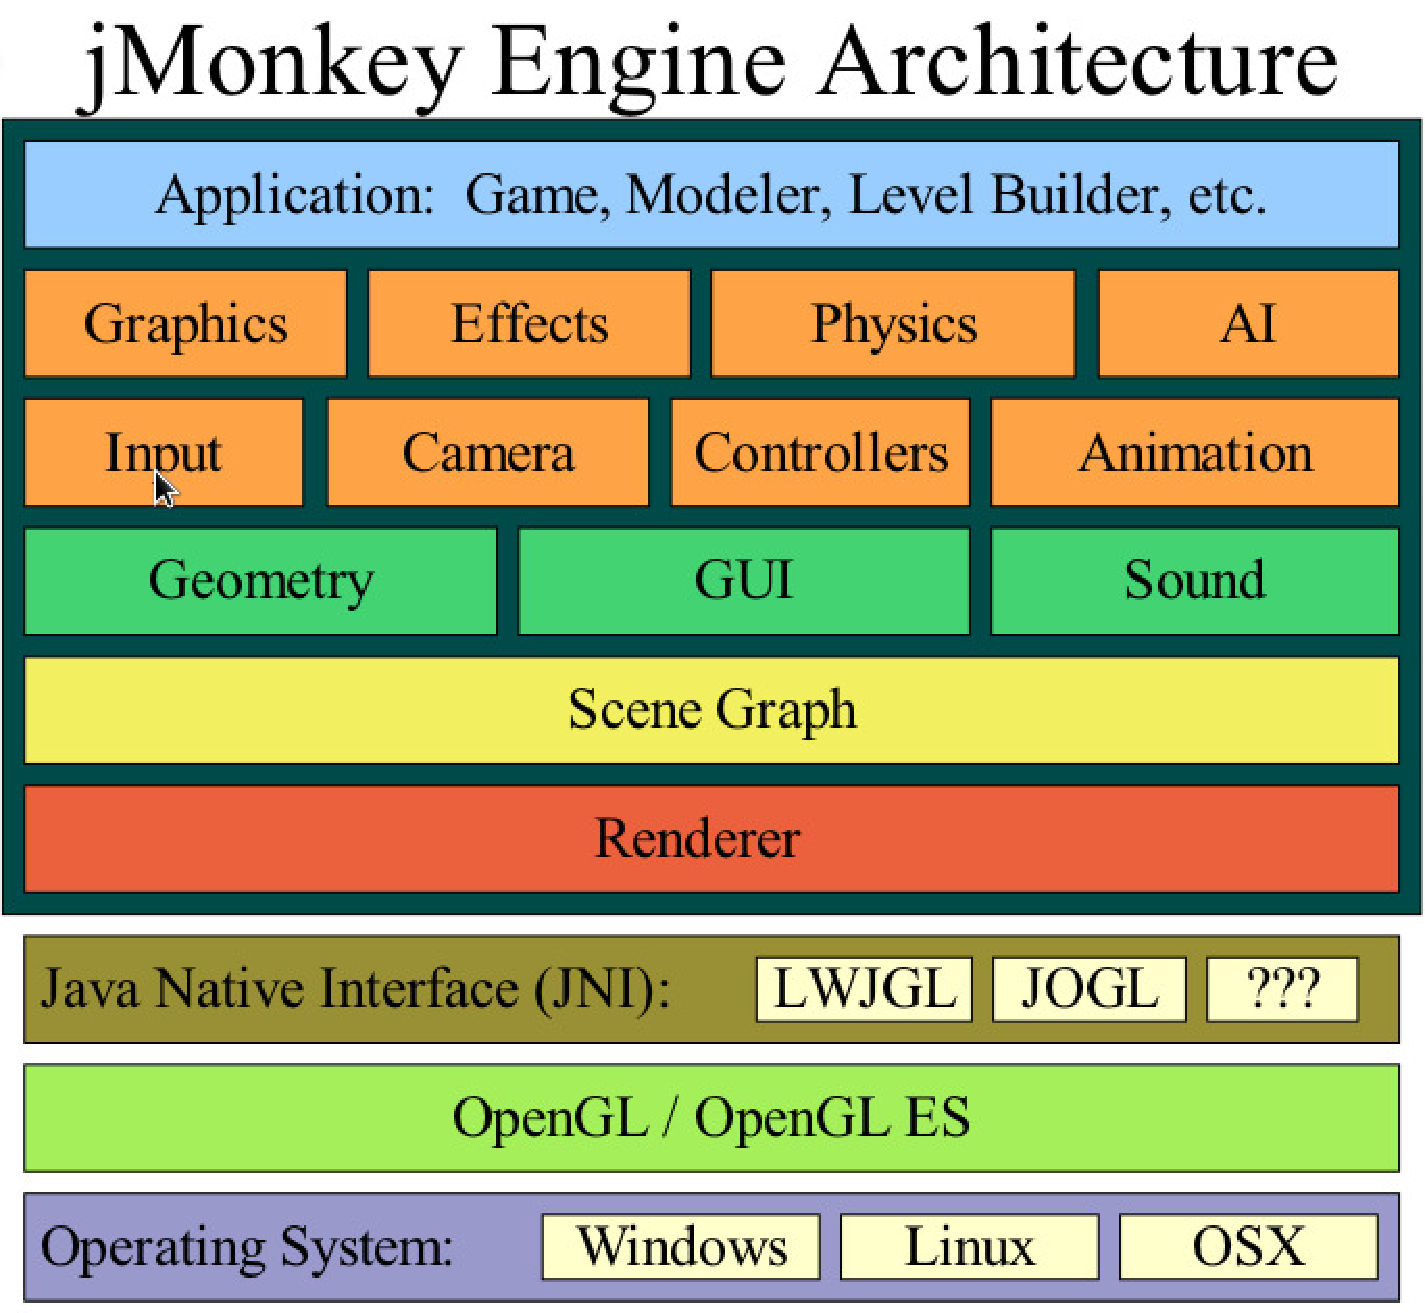
\includegraphics[scale=0.6]{arquitectura.pdf}
\caption{Arquitectura de motor jMonkeyEngine}
\label{archjme}
\end{center}
\end{figure}
\subsection{Sistema Operativo}
JME está desarrollado completamente en Java, una plataforma independiente de cualquier Sistema Operativo por lo que cualquier aplicación desarrollada con esta tecnología será capaz de ejecutarse en los sistemas operativos actuales más conocidos como GNU/Linux, MacOS, Microsoft Windows, Solaris y cualquier otro que soporte la tecnología Java. 

Sin embargo, el acceso a recursos definidos por OpenGL y OpenAL\footnote{Del inglés Open Audio Library (\textit{Librería de Audio libre})} son completamente dependientes del sistema operativo, y es por ello que JME se vale de otras librerías para acceder a estos recursos. LWJGL\footnote{Del inglés Lightweight Java Game Library, (\textit{Librería de juegos liviana de java})} es una de ellas, esta funciona en todos los sistemas operativos antes mencionados dado que también está desarrollada en Java, sin embargo ésta utiliza JNI\footnote{Del inglés Java Native Interface (\textit{Interfaz nativa Java})}, un framework que permite acceder a programas escritos en lenguajes de bajo nivel tales como C/C++ por lo que actúa como puente entre el motor con OpenGL y OpenAL.
\subsection{OpenGL}
Como se ha mencionado antes, OpenGL es una API estándar multilenguaje y multiplataforma para el desarrollo de aplicaciones gráficas. 

El hecho de que sea una especificación permite que los fabricantes del hardware realicen sus implementaciones en base a este estándar y luego los desarrolladores se abstraigan del acceso a las diferentes tarjetas, ya que la forma de trabajar será siempre la misma, para tarjetas diferentes (que cumplan con el estándar por supuesto).

OpenGL ES\footnote{Del inglés OpenGL for Embedded Systems (\textit{OpenGL para Sistemas embebidos})} es la API embebida para dispositivos móviles, consolas, celulares etc. LWJGL planea dar soporte a este estándar, por lo que permitirá a todas las aplicaciones desarrolladas con JME puedan ser ejecutadas sin ningún problema en dispositivos móviles.
\subsection{Java Native Interface (JNI)}
JNI es el puente entre LWJGL y OpenGL. A través de éste es posible acceder a las funciones de OpenGL, sin embargo, dado la arquitectura modular en la que ha sido desarrollado el motor, permite que alguna otra librería de acceso a OpenGL pueda ser usada sin romper la estructura del motor. Una posible futura implementación puede ser JOGL (\textit{Java OpenGL}) que está siendo desarrollada aún por la JCP (\textit{Java Community Process}) bajo la especificación JSR-231 \cite{JSR}.
\subsection{Renderer}
La siguiente capa es el renderizador. Renderizar una escena se refiere al proceso que genera una imagen a partir de un modelo de datos. El modelo de datos puede contener geometrías, texturas, intensidad luminosa y la información necesaria sobre cómo procesar dichos datos. 

Por lo tanto el renderizador tiene al menos 3 responsabilidades en JME:
\begin{enumerate}
\item Transformar los datos de la escena y llevarlos a un espacio plano de la pantalla.
\item Eliminar partes de la escena que no son necesarias, mejorando considerablemente el rendimiento. Esto puede hacerse a través de Culling o Clipping, ambos métodos serán descritos posteriormente. 
\item Dibujar la escena transformada en la pantalla.
\end{enumerate}
\subsection{Grafo de escena (Scene Graph)}
El gráfico de escena es la estructura de datos que almacena todos los objetos que deberán ser dibujados. La implementación del gráfico de escena de JME tiene una estructura de árbol, es decir está formado por un conjunto de nodos padres e Hijos, y también nodos finales llamados nodos hojas.

Los tipos de nodos por los que está compuesto el gráfico de escena son los siguientes:
\begin{description}
\item[Nodos padres] pueden tener cualquier cantidad de nodos Hijos. 
\item[Hijos] que sólo pueden tener un nodo padre.
\item[Nodo raíz] que no tiene nodo padre y es el nodo inicial del cuál inicia la jerarquía.
\item[Nodos hojas] que son los que tienen las figuras geométricas que serán renderizadas en la pantalla.
\end{description}
Existen muchos beneficios de tener el gráfico de escena en el motor, entre ellos se destacan los siguientes:
\begin{itemize}
\item Simplifica enormemente la gestión de todos los atributos: Por ejemplo para establecer la efectos de luz a los atributos o geometrías de una escena basta con establecerla sólo al padre de todos los Hijos, y no a cada hijo por separado.
\item Permite la agrupación de los objetos en la misma región espacial: Esto es muy eficiente para el descarte de objetos que no necesitan ser procesados, de manera que se descarta todo un sub-árbol del gráfico de escena, de este modo se ignoran todos sus Hijos. 
\item Facilita la posición de una jerarquía de modelos, por ejemplo para el caso de un modelo de un humano, el torso determina la posición de los brazos, la cabeza y las piernas. Los brazos determinan la posición de las manos, y ésta la posición de los dedos, etc. 
\item Ayuda a la persistencia del juego, dado que al guardar el nodo raíz, se realiza un guardado recursivo de todos sus Hijos, y los Hijos de sus Hijos y así.
\end{itemize}
Anteriormente se habló de dos técnicas que se utiliza en el motor, Culling y Clipping. Ambas técnicas se utilizan para descartar objetos que a vista del observador no son visibles y por tanto no necesitan ser procesadas por el renderizador \cite{BEGINNERS}.

Mediante culling es posible descartar un conjunto de objetos que no necesitan ser renderizados. 
\\Por ejemplo, en una habitación hay un conjunto de objetos y todos ellos comparten un padre, en este caso la habitación. Todas las habitaciones comparten un padre, que puede ser el piso de un edificio. Todos los pisos comparten también un padre, el edificio. La jerarquía puede verse en la Figura \ref{culling1label}.
\begin{figure}[!hbp]
\begin{center}
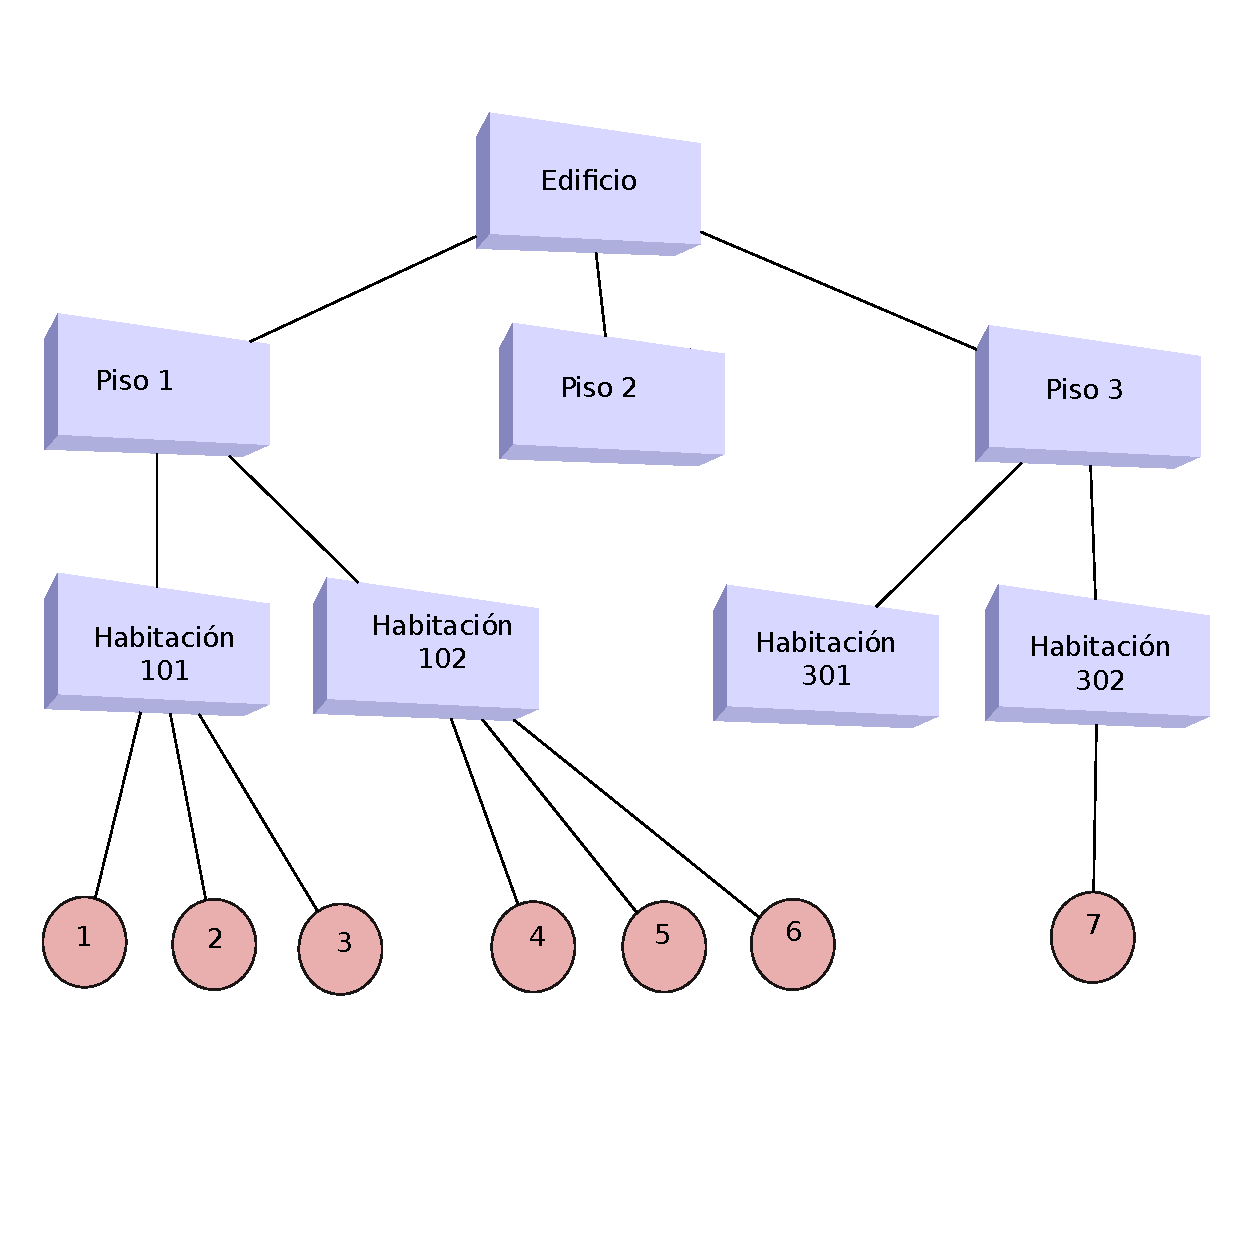
\includegraphics[scale=0.7]{culling1.pdf}
\caption[Ejemplo Culling 1]{Jerarquía de objetos en el gráfico de escena}\label{culling1label}
\end{center}
\end{figure}

Si se necesitara renderizar una escena donde un individuo (el observador) estuviese dentro de la habitación 302 del piso 3 del edificio, sólo sería necesario procesar una rama en particular de toda la jerarquía, lo que se muestra en la Figura \ref{culling2label}.
\begin{figure}[!hbp]
\begin{center}
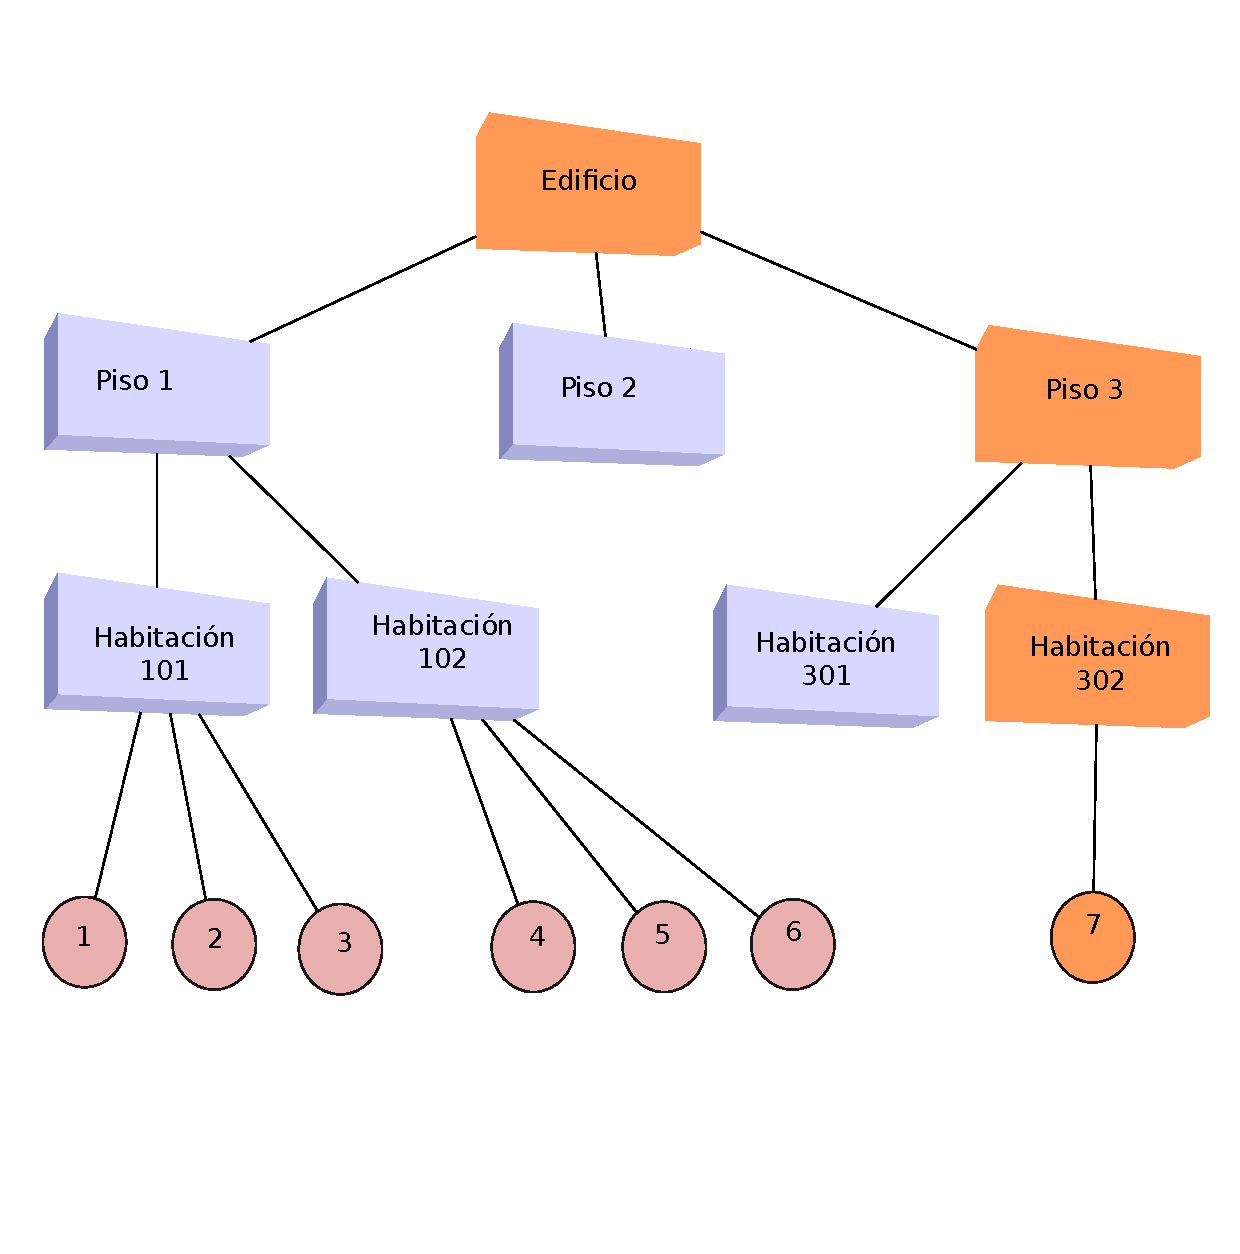
\includegraphics[scale=0.7]{culling2.pdf}
\caption[Ejemplo Culling 2]{Jerarquía de objetos en el gráfico de escena}\label{culling2label}
\end{center}
\end{figure}

La rama marcada con naranjo indica la rama a ser procesada, y en este caso el nodo hoja (7) de la habitación 302 del piso 3 del edificio será el objeto renderizado, descartando todas las demás ramas, finalmente todo esto se traduce en una mejora en rendimiento dado que la cantidad de nodos a procesar disminuye considerablemente. 

Para el caso de Clipping es bastante similar, sólo que en vez de trabajar con ramas, se hace directamente con los objetos, y los divide en partes más pequeñas, determinando entonces cuáles partes del objeto deben ser las dibujadas. 
\subsection{Geometrías}
Las geometrías son los nodos hojas dentro del gráfico de escena y son los objetos que finalmente son dibujados en la pantalla. Éstos contienen los datos necesarios para poder renderizar los objetos, gestionan toda la información tales como materiales que son las que describen qué y cómo debería ser renderizada la superficie de la geometría \cite{BEGINNERS}.
\subsection{Interfaz gráfica del usuario (GUI)}
La interfaz gráfica de usuario en el motor está soportada por nifty- gui, un proyecto independiente que está orientado a proveer un conjunto abundante de componentes gráficos para aplicaciones generales y juegos en general. Ésta está desarrollada en Java y también hace utilización de OpenGL para el renderizado de las imágenes a través de LWJGL.

Nifty-gui utiliza un archivo de configuración en formato XML para definir la posición de sus componentes como la pantalla, las capas, texto, paneles, etc. Esta interfaz no pretende ser un framework como Swing o AWT de Java, pero sí pretende hacer la interacción con el usuario mucho más amistosa y personalizada a la aplicación o juego en la que se esté utilizando. 
\subsection{Sistema de sonido}
El sistema de sonido que utiliza JME es similar en arquitectura al renderizador en donde los sonidos son renderizados pensando en un espacio 3D. Al menos 2 tipos de interfaces a nivel de código se utilizan para el sistema de sonido:
\begin{enumerate}
\item ISoundSystem: Se encarga de controlar y gestionar todos los sonidos realizados durante el juego. 
\item ISoundRenderer: Es el renderizador del sonido que lo conecta al gráfico de escena. Esto da la sensación por ejemplo si en el juego pasara un objeto volador como un avión, entonces el renderizado permitirá oír el sonido como si el avión pasara y se alejase de nuestra ubicación actual. 
\end{enumerate}
\subsection{Gráficos, Efectos, Entradas, Cámara}
Las capacidades gráficas del motor son bastante buenas y aceptable a pesar de que el motor se considera en estado Alpha, actualmente las capacidades le permiten lo siguiente:
\begin{itemize}
\item Utiliza Shaders, lo que nos permite trabajar con lenguajes de sombreado y aplicarlo a los modelos utilizados por el motor.
\item Utiliza variados tipos de efectos de luz como colores sólidos, transparencias, reflexión, etc. Entre ellas se destacan las siguientes \cite{JMONKEY} 
\begin{itemize}
\item Diffuse Map
\item Alpha Map
\item GlowMap
\item Bump Map
\item Specular Map
\item Parallax Map
\end{itemize}
\item Renderización de texturas y soporte multi- texturas
\item Diversos cargadores de modelos
\begin{itemize}
\item MilkShape modeler
\item ASE: 3D Studio Max modeler.
\item MD2: Formato de modelos del juego Quake2
\end{itemize}
\item Varias primitivas construidas por defecto, como líneas, puntos, cubos, triángulos, esferas, etc. 
\end{itemize}
En cuanto a los tipos de efectos, posee de tipo partículas entre los que destacan explosiones, fuego, humo, etc. Y efectos 2D como efectos de agua, reflejos de agua, luz solar, niebla, manchas, etc \cite{JMONKEY}. 

El sistema de cámara es el que permite proyectar los objetos a la pantalla. El sistema completo está compuesto por 4 componentes:
\begin{description}
\item[Eye Point] Es la localización actual de la cámara.
\item[View Plane] Es el plano en donde los objetos son proyectados.
\item[Viewport] Es la región de interés del View Plane, y se considera el foco de la escena. 
\item[View Frustum] Es el componente que permite realizar Culling y Clipping. 
\end{description}
Las entradas aceptadas de momento son los Joystick, Mouse y Teclado.
\subsection{Nivel superior}
En el nivel superior están todas las demás aplicaciones que se basan en el motor, creando así nuevamente una nueva capa y posiblemente algunas de éstas podrán establecer la base para poder crear otras aplicaciones. Ejemplo en este nivel están los juegos, aplicaciones de modelado, aplicaciones CAD etc.

Este proyecto se considera una de esas aplicaciones que se basan en todas las demás capas anteriormente mencionadas, sin embargo no establecerá ningún marco de extensión para que pueda considerarse como un nuevo nivel. 
\chapter{Descripción del juego}
El nombre del videojuego es jBomb. El proyecto está basado en la idea de un videojuego de tipo Shooter\footnote{Generalmente se les dice Shooter a juegos en primera persona donde el principal objetivo es atacar a enemigos mediante algún arma, juegos tales como Quake, Counter Strike, Medal Of Honor, etc.} y que se asemeja al juego Bomberman\footnote{Videojuego estratégico desarrollado por Hudson Soft}. A diferencia de este último, jBomb pretende aumentar la jugabilidad sin importar dónde se encuentren los jugadores, es decir el juego está orientado a ser jugado en red la cual puede ser una red local o bien a través de Internet.

A pesar de que jBomb implementa la idea general de Bomberman, éste tiene sus propias características que no están en Bomberman, así como también este último tiene características que no son implementadas por jBomb. 

El juego tiene características de los juegos actuales entre las que se destacan los gráficos 3D y la jugabilidad en red. Además está ambientado en un entorno espacial acompañado de música electronica lo que da una sensación de juego futurista.

A pesar de lo anterior el juego es un proyecto pequeño de poca envergadura en comparación a los juegos actuales, sin embargo los mismos pricipios comunes para cualquier juego son aplicados.
\section{Objetivos}	
El estilo de juego es por rondas y el objetivo es sobrevivir a esas rondas. Para llevar a cabo esto el jugador debe defenderse de la mejor manera posible frente a los ataques de los otros participantes, además de atacarlos. Este objetivo es fiel al estilo Bomberman, sin embargo en este último se lleva un conteo de cada ronda ganado por jugador, por lo que en algún momento se decide el quien es el ganador del juego en base al número de rondas ganadas anteriormente.
jBomb actualmente no lleva ningún registro de rondas por lo que el ganador se considera quien gane la ronda, luego el juego se reinicia y un nuevo ciclo se inicia.
\section{Características}
\subsection{Gráficos 3D}
Una de las características más significativas del juego es que cumple con un requisito casi fundamental para la mayoría de los usuarios: su gráfica ha sido desarrollada en 3 dimensiones. Esto no necesariamente ha sido fiel al estilo de Bomberman dado que este último es un juego antiguo que posee gráficos solamente en 2 dimensiones.

\begin{figure}
\begin{center}
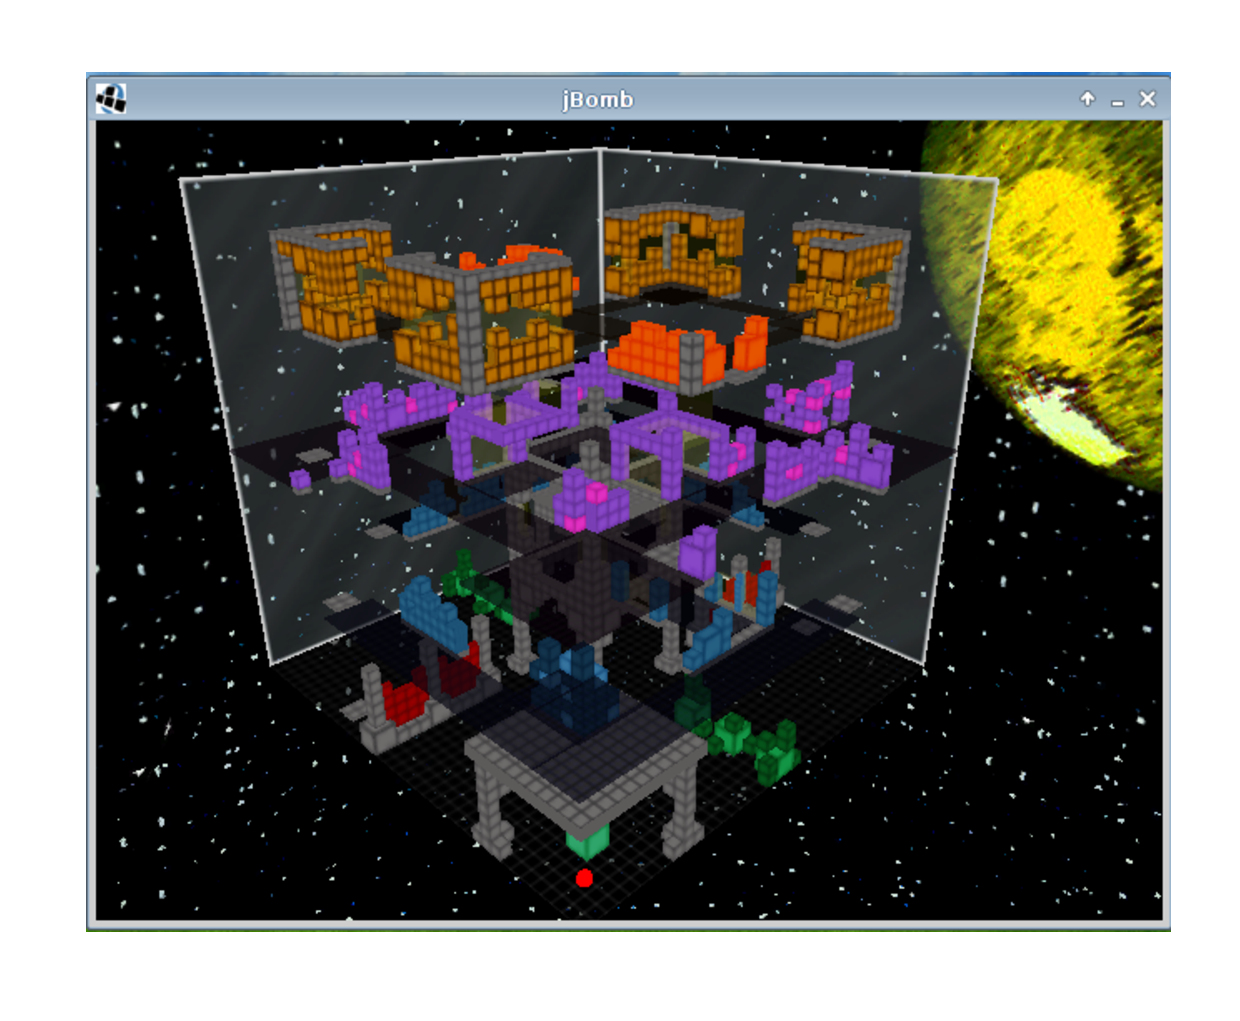
\includegraphics[scale=.7]{img1.pdf}
\end{center}
\caption[Cubo de escenario]{Toda la acción de jBomb ocurre en un cubo de vidrio}
\end{figure}

jBomb agrega esta característica para acercarse al nivel de los juegos actuales pero su jugabilidad es representativo de un estilo retro, donde la simpleza se hace presente en sus mecánicas de juego, en la interfaz del jugador y en su objetivo. En la Figura \ref{trilabel} se muestra parte del escenario principal de jBomb.

\begin{figure}
\begin{center}
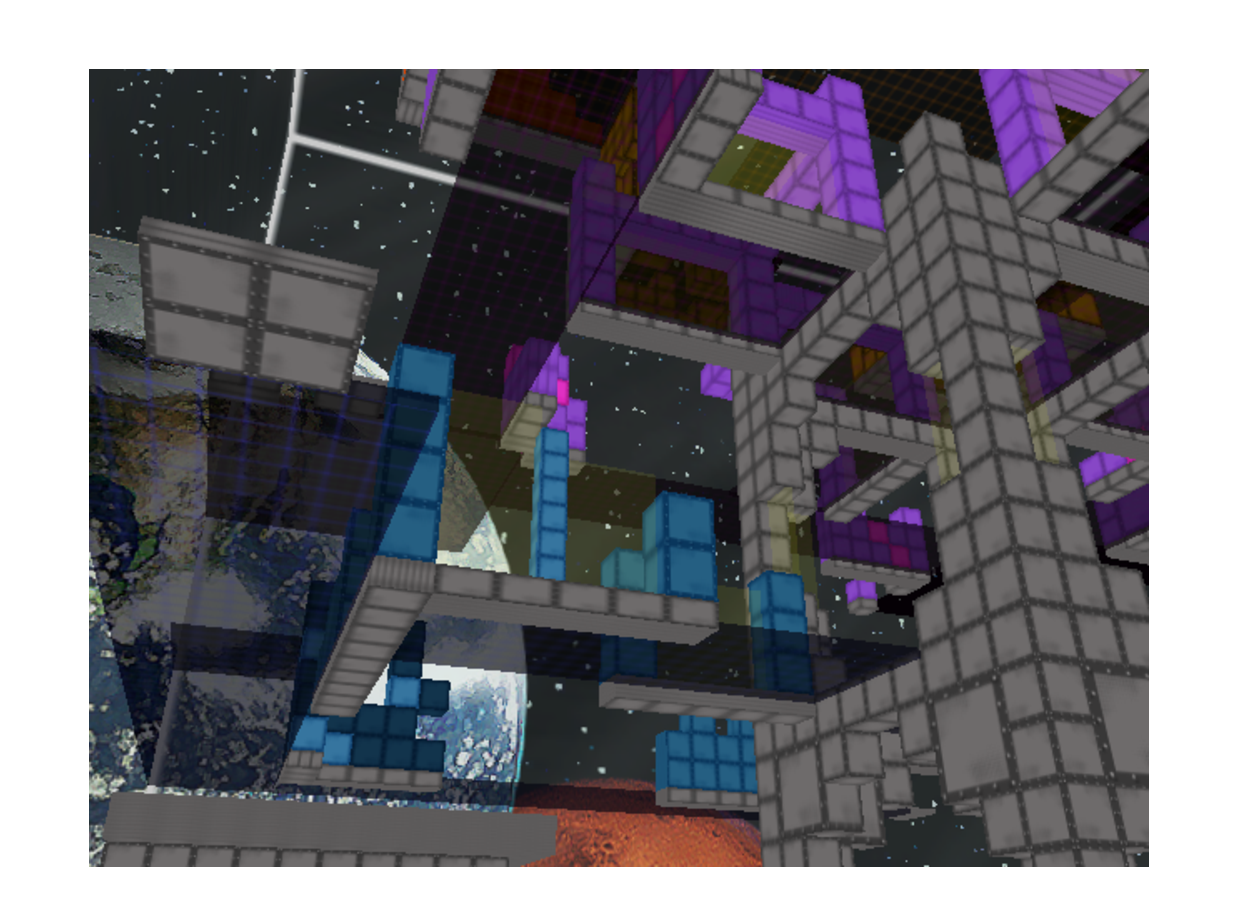
\includegraphics[scale=.7]{tri.pdf}
\end{center}
\caption[Imágen de escenario 3D en jBomb]{Se muestra el escenario principal de jBomb con gráficas en 3D}
\label{trilabel}
\end{figure}
\subsection{Primera persona}
Dado que el juego se desarrolla en un ambiente en 3 dimensiones, la perspectiva del usuario en el escenario es en primera persona, lo que le permite al jugador tener una impresión más real sobre el juego. Esto es así para todos los jugadores, por lo que un mismo escenario es visto de distinta forma en el espacio.

Esta es la característica que se le atribuye a los juegos de tipo Shooter, donde la forma de interactuar con el juego hace que fuese el propio jugador el que está en la escena. Existe una infinidad de juegos de este tipo, pero jBomb en un comienzo trató de simular tales características parecidas a las del juego Counter Strike, de la empresa Valve.
\subsection{Juego en red}
Una de las características más importantes del juego es la forma en la que participan los jugadores. Bomberman se ejecutaba en consolas como Nintendo y Super Nintendo y a pesar que los participantes en el juego eran 4, sólo 2 podían ser controlados por las personas dado que las consolas ofrecían 2 mandos de juego. Aún así se desconoce si el juego fue extendido a otras consolas o si se desarrolló un mecanismo que permitiese a los jugadores participar todos a las vez.

En jBomb, los jugadores no tienen que estar físicamente en el mismo lugar para poder participar en el juego, dado que éste permite ser ejecutado en red con una arquitectura Cliente-Servidor \cite{VALVE1}.\\
Esto permite descentralizar el juego de tal manera que el servidor puede ser iniciado en una máquina totalmente independiente de los jugadores, y éstos a su vez pueden estar en cualquier máquina que esté conectada a internet o bien a la red local. Como se dijo anteriormente, ésta es la característica más potente y valiosa que posee el juego, porque su implementación tiene un fuerte impacto en la satisfacción del usuario.
\subsection{Ambiente}
jBomb tiene un estilo espacial y es por ello que tanto las texturas \cite{GB} utilizadas en el juego, así como las propiedades que forman el fondo tienen imágenes de planetas y estrellas, además la música utilizada para el acompañamiento del juego es de tipo Electrónica, diseñada especialmente para jBomb. Esta característica hace que el juego tenga un estilo futurista.

Las Figuras \ref{sky1label} y \ref{sky2label} muestran un par de imágenes utilizadas en el fondo de horizonte del juego.
\begin{figure}
\begin{center}
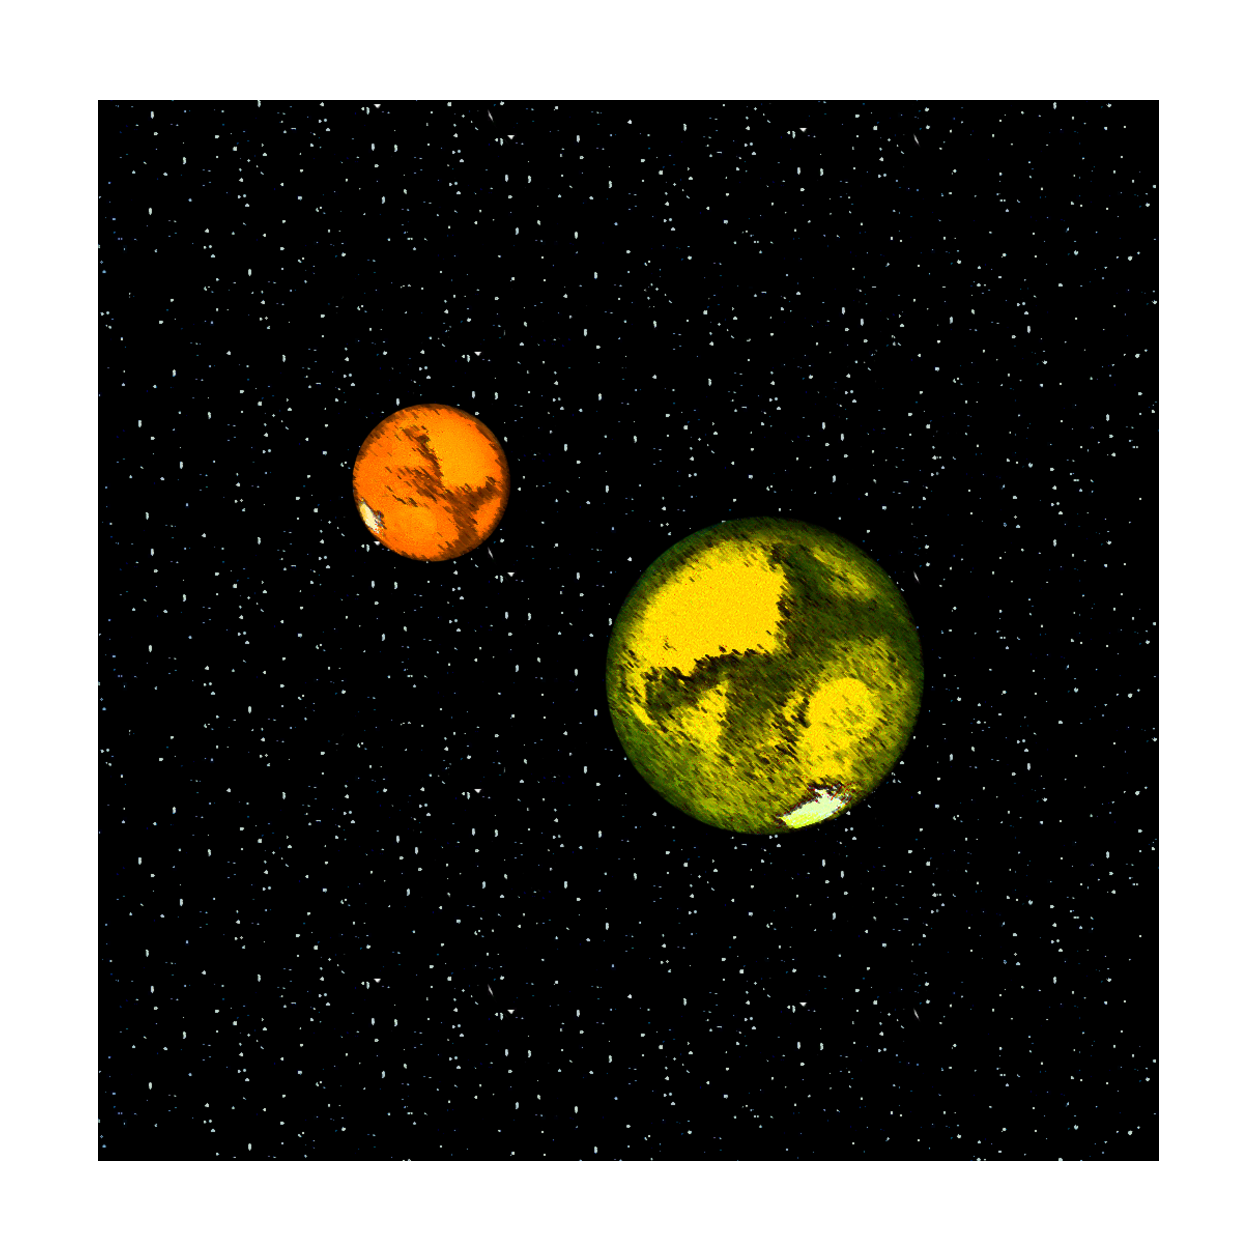
\includegraphics[scale=.7]{sky.pdf}
\end{center}
\caption[Fondo espacial utilizado en jBomb (1)]{Fondo espacial utilizado en jBomb, corresponde al horizonte del juego \cite{GB}}
\label{sky1label}
\end{figure}
\begin{figure}
\begin{center}
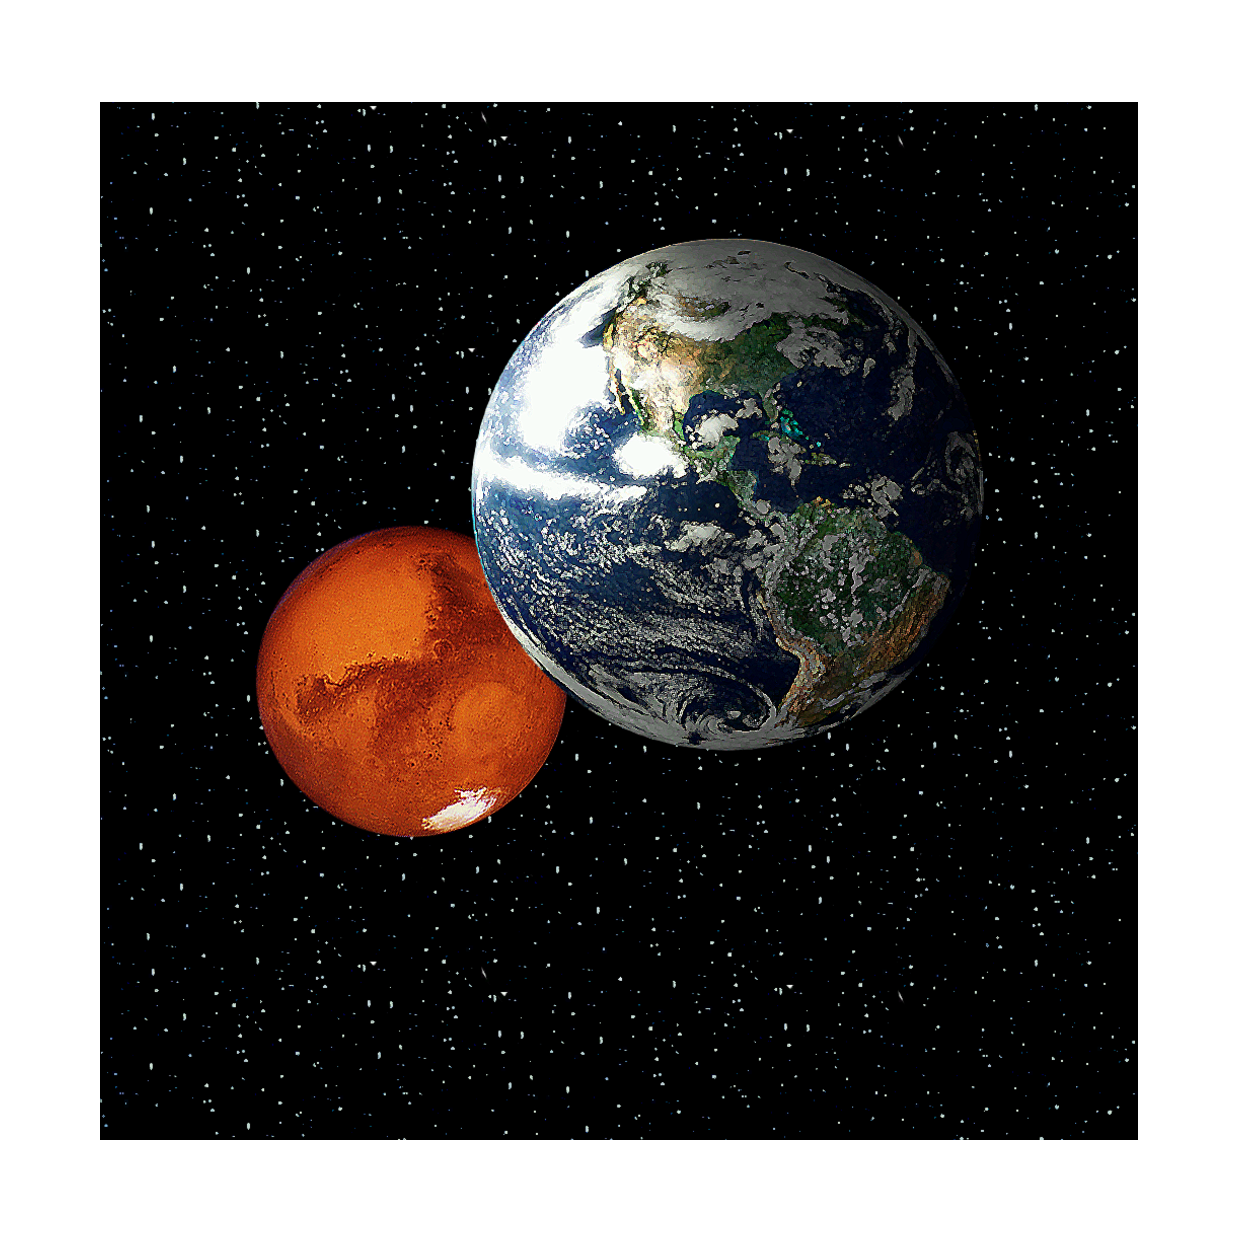
\includegraphics[scale=.7]{sky2.pdf}
\end{center}
\caption[Fondo espacial utilizado en jBomb (2)]{Fondo espacial utilizado en jBomb, corresponde al horizonte del juego \cite{GB}} 
\label{sky2label}
\end{figure}
\subsection{Interfaz de información}
jBomb implementa muchas de las características básicas que cualquier juego debe tener, y entre ellas está la interfaz de información \cite{BEGINNERS}.\\
Esta interfaz es la que le permite al usuario ver el estado actual del juego y de las reglas de este.

Por ejemplo, en ella se muestra la cantidad de bombas disponibles para el próximo ataque a realizar, el tiempo en que la bomba explotará, la energía actual de todos los jugadores presentes en la ronda y otra información relacionada el juego.

Esta interfaz tiene la particularidad de que a pesar de que forma parte del juego, en jBomb es sólo utilizada para mostrar información relevante y en ningún momento forma parte del escenario ni afecta el comportamiento del juego. Ésta se limita exclusivamente a mostrar sólo la información pertinente al usuario en cuanto al estado del juego, así como también para informar cuándo una ronda está empezando o cuándo el jugador ha perdido.
\subsection{Perspectivas de espectador}
El objetivo principal del jugador es participar en la ronda y tratar de lograr la victoria. Sin embargo el juego es en línea y colaborativo, todos los jugadores son personas reales por lo que una vez que algún jugador pierda el juego no puede ser reiniciado porque los demás aún están en la ronda.

Cuando el jugador pierde, se realiza un cambio en la perspectiva del jugador, pasa de un estado de participante a espectador que le permitirá ver en tiempo real que sigue sucediendo en la ronda actual. La perspectiva de espectador permite al jugador moverse libremente por el escenario pero sin tener influencia en este, es una representación casi como la de un fantasma.

\begin{figure}
\begin{center}
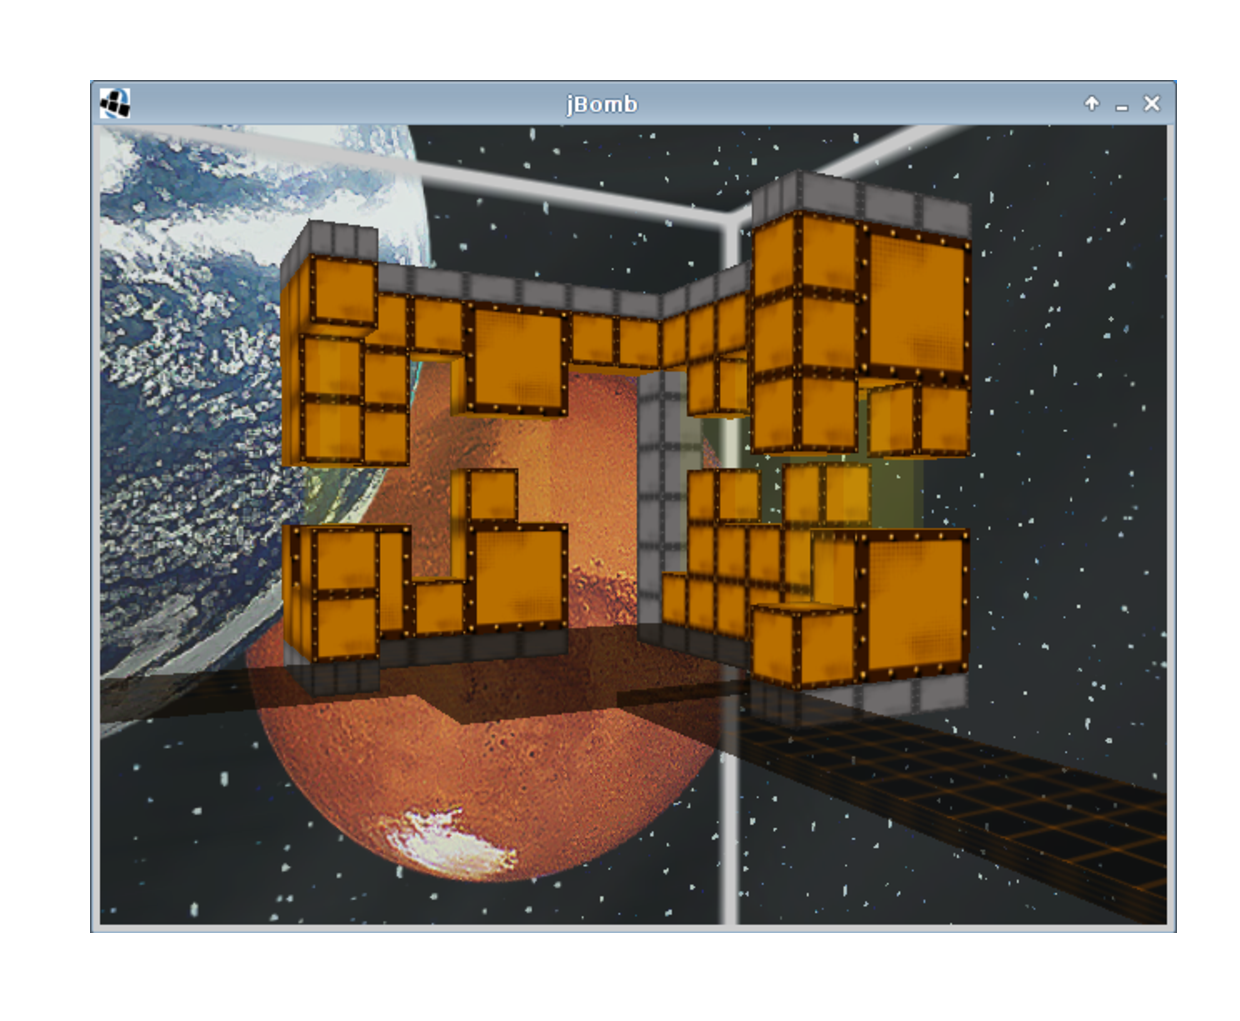
\includegraphics[scale=.7]{img2.pdf}
\end{center}
\caption[Escenario principal, cuarto nivel]{Escenario principal, cuarto nivel}
\end{figure}

En este sentido, esta es una característica que fue integrada a partir de la experiencia de los desarrolladores de jBomb con el juego Counter Strike, el cual implementaba la misma funcionalidad cuando el jugador habia perdido en la ronda actual.

Todo lo anterior sucede en el lado del cliente, sin embargo el servidor también puede ser ejecutado de dos formas distintas:
\begin{enumerate}
\item Headless: Esta forma de ejecución funciona como la mayoría de los servidores, en donde no hace falta la parte visual para llevar un registro de lo que está sucediento, donde el comportamiento y flujo de éste es informado mediante los mensajes de logs. 

Esto es así porque el servidor una vez que es ejecutado, no necesita ser manipulado para su funcionamiento, éste se encarga de gestionar todo automaticamente.
\item Display: Esta forma de ejecución difiere de la anterior sólo en que ahora se cuenta con una perspectiva de espectador de todo el juego, así el administrador puede ver en tiempo real qué está sucediendo en la escena.

Esta característica se agregó con la finalidad de depurar el juego y poder ver que el servidor mostraba realmente lo que estaba sucediendo con cada uno de los jugadores, una vez implementado, se dejó para poder registrar qué sucedía en el escenario. Pasó de ser una característica como apoyo para el desarrollo a ser una característica de juego.
\end{enumerate}
\subsection{Gestión de jugadores}
jBomb funciona en base al modelo Cliente-Servidor y gracias a ello el juego puede ser jugado a través de Internet. Esto hace que la complejidad del desarrollo del juego aumente porque se debe lidiar con problemas relacionados con redes. Uno de esos problemas pueden ser las conexiones y desconexiones de los jugadores con el servidor \cite{VALVE1}.

jBomb maneja muy bien este problema y se encarga de continuar con el juego cuando sucede una desconexión de jugador, siempre y cuando sea posible y tenga sentido, ésto sin perjudicar a los demás usuarios.
\subsection{Multijugador} 
jBomb puede ser personalizado para jugar con distintas cantidades de jugadores en línea. Las posibilidades actuales son iniciar el servidor con 2, 3 o 4 jugadores simultáneos. En este sentido se asemeja a Bomberman en donde la cantidad máxima de jugadores también era 4.
\subsection{Software Libre}
Esta es una característica que tal vez no es muy importante para los usuarios del juego, pero si lo es para los desarrolladores de juegos.
El beneficio para los jugadores de jBomb es que éste puede ser descargado desde la página de descarga de forma completamente gratuita\footnote{https://github.com/downloads/rvillablanca/jbomb/jbomb.zip}, nunca habrá un costo asociado por la utilización del juego, en ninguna de sus dos versiones (cliente y servidor).

\begin{figure}
\begin{center}
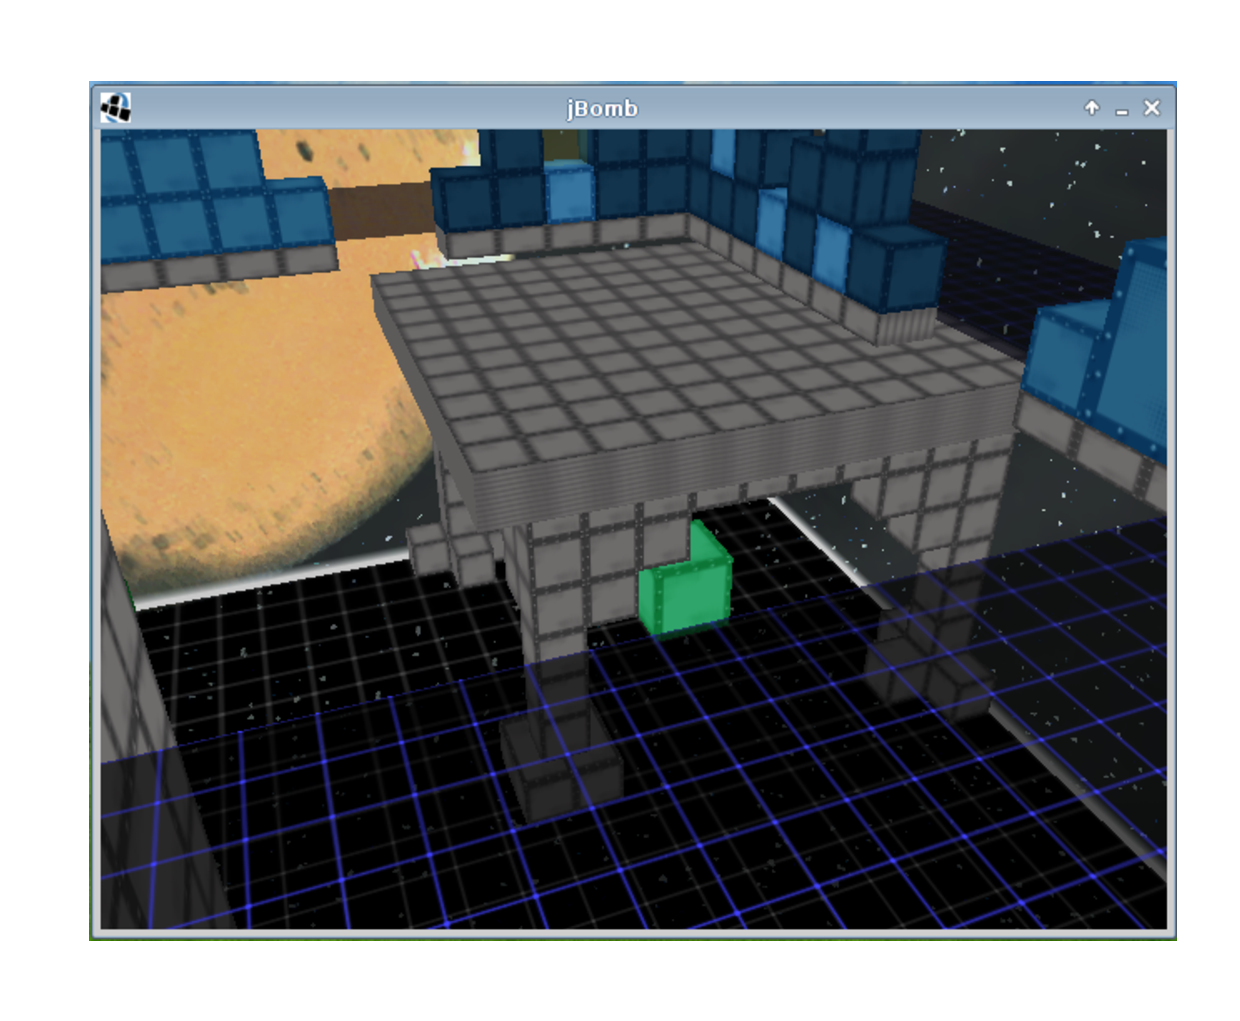
\includegraphics[scale=.7]{img3.pdf}
\end{center}
\caption[Escenario principal, segundo nivel]{Escenario principal, segundo nivel}
\end{figure}

Por otra parte, las personas que tengan la intención de aportar con el juego serán bienvenidas,  éstas pueden ser Desarrolladores, Ingenieros en diversas áreas, especialistas en sonido, diseñadores, etc. Además cualquier desarrollador o persona interesada tiene la posibilidad de tomar el juego y será libre de modificarlo, mejorarlo, e incluso crear su propio juego en base a jBomb.
\section{Mecánicas de juego}
Las mecánicas de juego son las reglas que están implementadas en el juego y definen la forma en cómo se interactua con éste. En la Figura \ref{meclabel} se muestra cómo GUI Node se encarga de informar el estado actual de algunas mecánicas de juego, por ejemplo el número de bombas disponibles, el tiempo de explosión de las bombas y un indicador de energía por cada jugador en la ronda.

\begin{figure}
\begin{center}
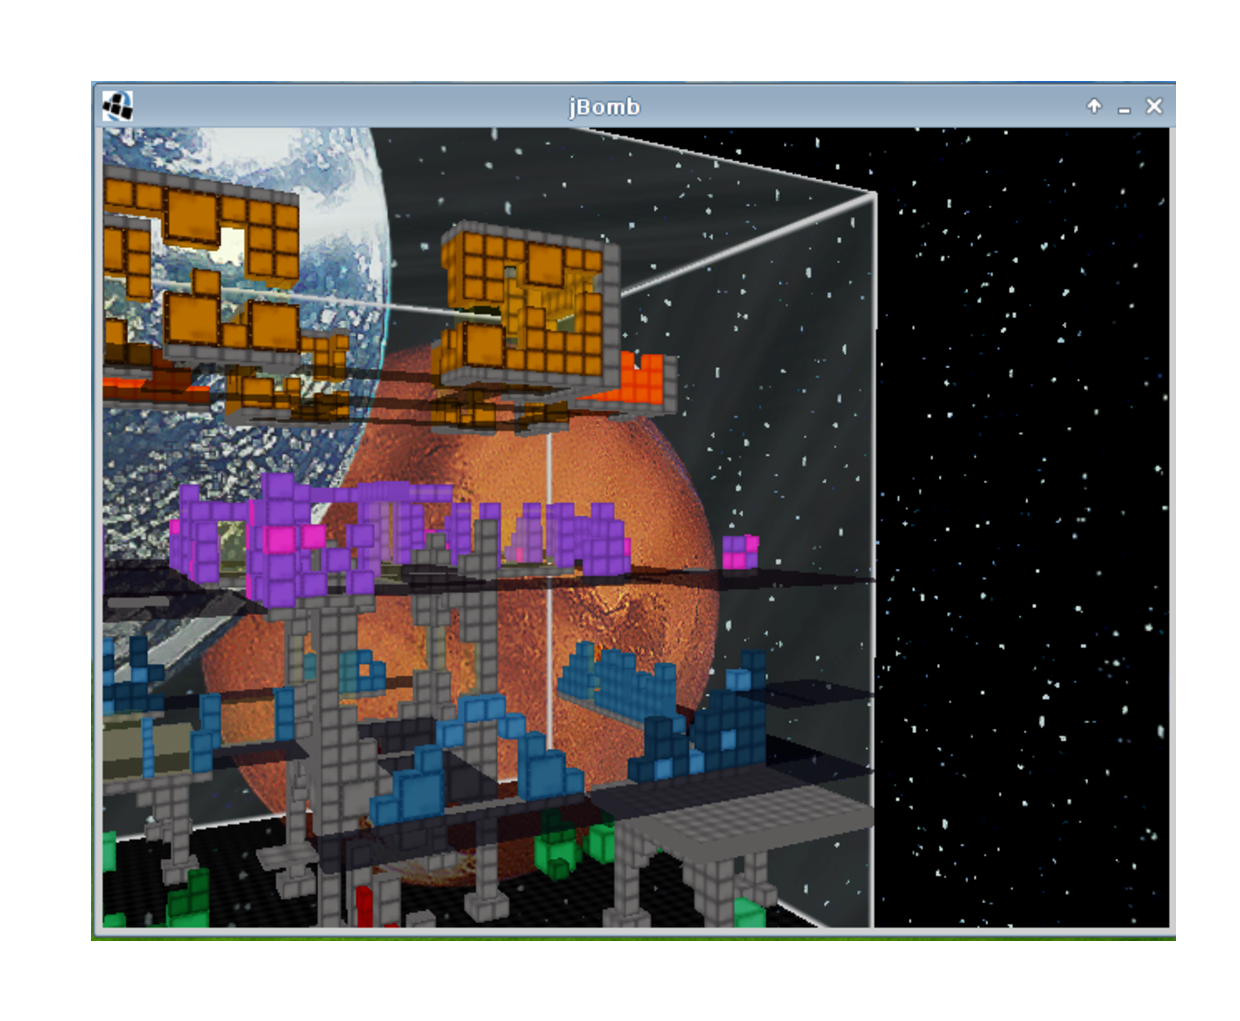
\includegraphics[scale=.7]{img4.pdf}
\end{center}
\caption[Escenario principal, perspectiva de espectador]{Escenario principal, perspectiva de espectador cuando jugador ha perdido}
\end{figure}

Para jBomb, existen al menos 3 mecánicas de juegos importantes.
\begin{enumerate}
\item Bombas por jugador: En jBomb la única arma que sirve para el ataque es la bomba, y por cada jugador sólo pueden haber un máximo de 3 bombas que pueden ser lanzadas seguidamente una tras otra, al cabo de un tiempo las bombas serán recargadas y el jugador las tendrá disponible para iniciar un nuevo ataque.
\item Duración de bombas: El jugador tiene la opción de lanzar la bomba con una duración que indica cuándo la bomba explotará, siempre y cuando ésta no haya colisionado antes con algún jugador, incluyendo al propio jugador. Los valores posibles de duración se miden en segundos y pueden ser 1, 2 o 3 [seg].
\item Energía del jugador: La energía de los jugadores se mide en porcentajes. Todos los jugadores comienzan con una energía inicial de 100\% y al llegar a 0\% pierden la ronda.\\		
Esta energía se va viendo afectada por los reiterados ataques de bombas recibidos, donde la colisión con ella o bien la explosión de ésta cerca del jugador causará una disminución de la energía del jugador. La bomba tiene un radio de explosión de 10 [mts], por lo que si el jugador está dentro de ese radio, se verá afectado.
\item Recuperación de bomba: Por cada bomba que lance el jugador, se debe esperar 5 segundos a que esta pueda volver a estar disponible para que pueda ser lanzada nuevamente. El tiempo es independiente entre una bomba y otra.
\end{enumerate}
\begin{figure}
\begin{center}
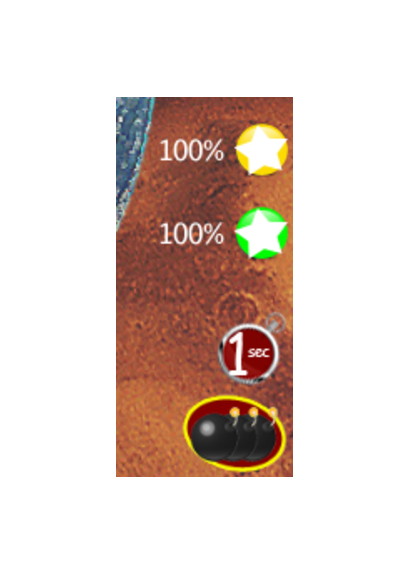
\includegraphics[scale=.7]{mec.pdf}
\end{center}
\caption[Mecánicas de juego]{Imágen que muestra cómo se informa el estado actual de las mecánicas de juego}
\label{meclabel}
\end{figure}
\chapter{Herramientas de trabajo}
Para el desarrollo del juego se utilizaron diversas herramientas con distintas funciones. La mayoría de ellas tienen una característica común, muchas son herramientas Open Source (código abierto). De hecho, por esta misma razón, jBomb nace como proyecto de código abierto dado que su desarrollo y gestión fue realizado en su mayoría con herramientas libres.

Algunas herramientas utilizadas tienen que ver con la gestión de todo el proyecto, otras están relacionadas completamente con la automatización del proceso de desarrollo del juego, y por último algunas herramientas fueron utilizadas para proporcionar recursos tales como imágenes en el juego.

Las herramientas utilizadas para la realización del proyecto fueron las siguientes:
\begin{description}
\item[NetBeans 7.1] Entorno de desarrollo integrado.
\item[Java] Lenguaje de desarrollo y plataforma sobre la que se ejecuta el juego.
\item[Subversion] Sistema de control de versiones para el código fuente del proyecto.
\item[Google Code] Sistema de gestión proyectos de software.
\item[Photoshop] Famoso editor gráfico.
\item[Gimp] Editor gráfico de imágenes.
\end{description}
Otras que se pueden considerar como librerías sobre las que se apoya jBomb tales como:
\begin{description}
\item[LWJGL] Librería libre que permite acceso a OpenGL a través de Java.
\item[Log4j] Framework especializado para Logs en Java.
\item[JMonkeyEngine] Motor de juegos para la plataforma Java.
\end{description}
\section{Herramientas}
\subsection{NetBeans}
NetBeans es un entorno de desarrollo integrado diseñado especialmente para desarrollo de proyectos con el lenguaje de programación Java, sin embargo éste no se limita sólo a Java, actualmente soporta Javascript, PHP, Groovy, C, C++, Scala, Clojure y más.

NetBeans está desarrollado en Java y por tanto funciona en la mayoría de las plataformas, Windows, Linux, MacOS, Solaris y otros.
Esta herramienta permitió que el tiempo de desarrollo del proyecto se redujera debido a que posee características que automatizan muchos procesos.
\subsection{Java}
Java es el lenguaje de programación con el que se ha desarrollado todo el proyecto y es a su vez la plataforma de ejecución donde corre jBomb \cite{JAVA}. La utilización de Java en los tiempos actuales es muy extensa y tiene participación en diversos tipos de proyectos y segmentos del mercado, y en particular en todo tipo de proyectos de software empresariales.

Sin embargo su participación en el segmento de los juegos de computadores (PC) es bastante reducida o casi nula (no así en aplicaciones y juegos para plataformas móviles a través de su API JavaME y también la API de Android).
\subsection{Subversion}
Cuando se desarrolla un proyecto de software siempre es importante contar con algún respaldo del código fuente para no perder avances o incluso perder todo el proyecto. Cuando los proyectos son pequeños (en cuanto a su envergadura y al número de integrantes que conforman el equipo de desarrollo del proyecto) a veces no se ve tan clara la necesidad de contar con algún sistema de versiones.

Cuando el proyecto se estima que es de una gran envergadura debido a su estimación de tiempo y costo, además del capital humano que requerirá para su desarrollo se hace imprescindible la utilización de un sistema de control de versiones que permita llevar un seguimiento del desarrollo del proyecto, así como el respaldo de éste.

Un sistema de control de versiones es un software que permite llevar un seguimiento del desarrollo del proyecto que se está creando. Éste permite trabajar en equipo y evita muchos problemas relacionados con la sincronización del trabajo de las personas, y el versionado del código que se está desarrollando.

Existen varios sistemas de control de versiones conocidos, algunos de ellos son Subversion, Git, CVS, Bazaar, Mercurial, Perforce, etc. Muchos tienen similitudes y diferencias, pero tal vez la mejor forma de clasificarlos es mediante la forma en cómo se almacenan los archivos. Existen dos tipos: Sistemas Centralizados y Sistemas Distribuidos. No es objetivo de este trabajo detallar las ventajas y desventajas de cada uno, sólo detallar Subversion como sistema de control de versiones de jBomb el cual es un tipo centralizado.

Subversion trabaja de forma centralizada lo que quiere decir que siempre hay un sólo servidor que se encarga de realizar todo el trabajo, y los desarrolladores crean copias de trabajo que son idénticos al servidor, excepto por la cualidad de que éstas son solo copias y no servidores (a diferencia de lo que sucede con sistemas distribuidos).

Subversion permite llevar todo el software versionado, es decir que por cada cambio que sea realizado por algún desarrollador en el servidor se creará una nueva revisión del software a la que posteriormente podría volverse. Gracias a estos sistemas la colaboración entre cada integrante del proyecto se hace más fácil, permite saber en qué está cada integrante y también ofrecen diversas funciones como:
\begin{itemize}
\item Explorar remotamente los fuentes y archivos que están en el servidor
\item Subir cambios al servidor
\item Actualizar las copias de trabajo
\item Mezclar copias de trabajo
\item Crear ramas independientes de la rama principal y marcado de etiquetas para sucesos importantes
\item Ver diferencias entre las copias de trabajo y el servidor
\end{itemize}
Esas son sólo algunas de las funciones que nos ofrecen los sistemas de control de versiones, y en este caso en particular Subversion.
\subsection{Google Code}
Google Code es un sistema de alojamiento de proyectos libres. Este pone a disposición 3 tipos de sistemas de control de versiones, Git, Mercurial y Subversion. 

Además de ello, ofrece todo un sistema de gestión del proyecto e incluye diversas herramientas las que pueden ser utilizadas para realizar una Wiki\footnote{Generalmente se le denomina Wiki a un sitio encargado de proveer ayuda tales como docuentación, preguntas frecuentas, definiciones, etc. El ejemplo más claro es el sitio www.wikipedia.com, una enciclopedia en libre online} del proyecto, navegar a través de los fuentes del proyecto, controlar los bugs, cambios y nuevas funciones a través de un sistema de tickets, un sistema de publicación de descargas y por último todo un sistema de administración de los integrantes del proyecto, el licenciamiento del proyecto, niveles de funciones entre los participantes, etc.

Existen diversas alternativas a este tipo de herramientas, entre las más conocidas están GitHub, SourceForge y Google Code. La elección de Google Code fue realizada simplemente por previa experiencia con este sistema, pero GitHub últimamente ha credido rápidamente y ha superado en número de proyectos alojados a ambos sistemas antes mencionados y puede que en algún futuro se haga una migración hacia éste.

\subsection{Gimp y Photoshop}
Gimp y Photoshop son dos herramientas muy potentes y reconocidas en el mundo del software, especialmente por los diseñadores gráficos. Ambas herramientas están orientadas a la manipulación profesional de imágenes, aunque actualmente se puede hacer mucho más que eso. Photoshop es una herramienta propietaria de Adobe que trabaja sobre Windows y MacOS y es la herramienta más utilizada para trabajar con edición de imágenes.

Gimp es la alternativa libre a Photoshop y funciona sobre diversas plataformas, incluyendo Linux. En el proyecto ambas herramientas fueron utilizadas para crear todas las texturas del juego. Estas dos aplicaciones fueron las que menos se utilizaron, esto se debe a que formaron parte de el módulo de assets en el juego, lo que significa que se utilizaron solamente para trabajar con las imágenes y una vez terminadas no fue necesario trabajar sobre ellas nuevamente, a diferencia de los demás módulos que fueron cambiando en el transcurso del tiempo.

Ambas herramientas se utilizaron para afinar detalles en las texturas utilizadas, focalizándose sobre todo en las capa de transparencias.
Photoshop fue utilizado además para realizar el logotipo del juego.
\section{Librerías y Frameworks}
Anteriormente ya se había hablado sobre JMonkeyEngine y LWJGL, sin embargó se hará un resumen de cada una de las librerías utilizadas además de una librería especializada para hacer registros (logs) en el código, de manera que se pueda hacer un seguimiento del flujo de la aplicación.

Además se incluye la descripción de una librería que se utiliza implícitamente a través del motor llamada JBullet, la cual está encargada de realizar todo el comportamiento de simulación de físicas.
\begin{description}
\item[JMonkeyEngine] JMonkeyEngine es el motor de juegos que permite automatizar y facilitar las tareas involucradas en el desarrollo de un videojuego. A bajo nivel no es más que un framework que permite tal tarea \cite{JMONKEY}.
\item[LWJGL (Lightweight Java Game Library)] Esta es una librería que da acceso a todas las funciones primitivas de OpenGL, lo que permite al desarrollador aislarse aún más de la detalles específicos de sistema operativo a través de clases en Java. A pesar de que funciona como una librería, no es considerada un motor porque está un nivel más abajo y su principal función es abstraer al desarrollador sobre las funciones nativas de OpenGL \cite{LWJGL}.
\item[Log4j](Log for Java): Log4j es una librería que permite realizar registros o logs sobre el flujo de la aplicación. Es muy común que los desarrolladores utilicen ciertas sentencias que les facilitan la tarea de depurar sus proyectos, pero muchas veces esto deja dependencias entre el log y el código de producción, lo cual es algo que comúnmente no se desea porque estos registros son utilizados en su mayoría en modo de desarrollo \cite{LOG}.

La forma más simple de realizar registros es escribirlos directamente a la salida estándar (por lo general la pantalla) a través de funciones especiales, pero aunque esto sea correcto no es la manera más óptima de realizarlo porque conlleva mucho trabajo cuando no se desea utilizar más los registros, además comúnmente esas sentencias son compiladas y para borrarlas el código debe ser editado nuevamente \cite{LOG}.

Para evitar todo ese tipo de problemas, existen librerías especializadas que ayudan con este proceso y jústamente Log4j es una de ellas.
Una de las características de Log4j es que es altamente personalizable y muy fácil de controlar, además el control se puede llevar a través de archivos de configuración de tipo XML o archivos Properties\footnote{Archivos muy utilizados por Java definir configuraciones a través de pares de valores, un valor y una clave para acceder a dicho valor} y se evita el recompilado de los fuentes, y se permite un control de logs en tiempo de ejecución.
\item[JBullet] Ésta es un wrapper de la librería Bullet Physics Library (la cuál está implementada en código nativo) y es el equivalente a LWJGL pero para simulación de físicas. Esta librería no es utilizada directamente en el juego (al igual que LWJGL) pero se menciona porque es el núcleo de toda la funcionalidad que simula las fuerzas físicas en jBomb. El juego hace utilización extensiva de objetos físicos a través del motor, sin embargo éste a su vez utiliza JBullet para finalmente invocar a las funciones de la librería nativa.
\end{description}
\chapter{Metodología de trabajo}
Las metodologías de desarrollo de software nos permiten gestionar el proyecto de manera ordenada, es decir nos permite llevar muy bien los controles de tiempos o plazos, las delegaciones de tareas y responsabilidades, y permite que el proyecto se realice en los plazos establecidos por los clientes.

Las metodologías nos permiten conseguir el éxito en la realización de los proyectos, una de las formas más comunes de clasificarlas es según su forma de avance y trato con el cliente:
\begin{description}
\item[Metodologías Ágiles] Las metodologías ágiles están orientadas a desarrollar los proyectos a través de desarrollos funcionales en tiempos cortos que puedan ser verificados por el cliente, a esto se le denomina comúnmente iteración. Otro punto más sobre los que se centran las metodologías ágiles son el tratamiendo comunicacional cara a cara con el cliente, algo por sobre la documentación técnica sobre todos los procesos y procedimientos involucrados \cite{WIKIDS}.
\item[Metodologías estructuradas o tradicionales] Estas metodologías son totalmente lo contrario de las metodologías ágiles, mientras estas últimas son criticadas por su informalidad y falta de disciplina, las tradicionales promueven el desarrollo del proyecto de forma totalmente estructurada y predictiva, en el sentido que el avance va evolucionando a través de etapas consecutivas y para pasar a la siguiente no se puede avanzar si no está la etapa anterior realizada completamente. Además estas metodologías establecen que los requerimientos del proyecto deben ser establecidos con anterioridad y por tanto eso la hace menos flexibles y adaptables a los cambios \cite{WIKIDS}.
\end{description}
Sin embargo este proyecto tomó sólo algunas cosas de ambos tipos de metodologías porque ninguna de las dos se adapta a las necesidades que el proyecto requería. 

El proyecto siempre fue creciendo con cambios y estos iban apareciendo a medida que se avanzaba por lo que no era posible implementar una metodología tradicional, por otro lado en ningún caso el proyecto es debido a algún requerimiento, de hecho no se tiene trato con el cliente porque no hay clientes, y eso hace que no se necesiten entregables funcionales cada cierto tiempo. Es por esta razón que se opto por una metodología personalizada que está basada las dos anteriores pero sólo utilizando lo necesario para el desarrollo de jBomb.

La forma de trabajo en el proyecto siempre fue muy flexible con respecto a los días y tiempos de trabajo. En primera instancia había solo un desarrollador del proyecto quien es el autor del presente documento, y el desarrollo se realizaba en los ratos libres disponibles.
El desarrollo del proyecto comenzó definiendo objetivos generales semiflexibles ya que éstos podrían cambiar en alguna oportunidad y eran hacia dónde se quería llegar con el proyecto, estos objetivos fueron básicamente:
\begin{itemize}
\item Multiplayer (no necesariamente en red)
\item Juego tipo FPS
\item Juego en base a Bomberman
\end{itemize}
Todos éstos objetivos se cumplieron, pero también se agregarón más características que hicieron que el proyecto se transformara en algo más interesante para los jugadores, pero también triplico el trabajo necesario para el desarrollador. Una vez establecidos los objetivos generales se comenzó con el análisis y diseño de toda la estructura del proyecto. El aprendizaje de todas las herramientas y librerias utilizadas también se considera parte evolutiva del proyecto, ya que en ésto se invirtió cerca de un tercio del total de tiempo.

Una vez bien definidos esos objetivos y luego del análisis y diseño del juego en general, se comenzó el desarrollo principal del proyecto. En este sentido se trazó la línea que llevaría al cumplimiento de los objetivos generales y en el transcurso de ésta ocurrieron diversos sucesos, por ejemplo se integró un nuevo desarrollador llamado Diego Villablanca que apoyaría la parte gráfica y de escenario, además de poseer total independencia para implementar nuevas ideas o cambiar las que ya habían con respecto a esos dos temas.

Fue así entonces que en el desarrollo evolutivo aparecieron y desaparecieron nuevas ideas, mecánicas de juegos y el crecimiento del proyecto fue muy dinámico pero siempre con los objetivos generales claros. Esto se asemeja al la ruta que uno traza para llegar a algún lugar, en donde existen diversas maneras de hacerlo y no sólo una, en el camino pueden surgir desviós inesperados. Así fue cómo sucedio con el proyecto, cada vez se tuvo que hacer desvíos porque algunas ideas no estuvieron bien pensadas o bien fueron apareciendo algunas mejores, pero el destino siempre fue el mismo.

En cada día de trabajo, se adoptó una forma de trabajo en donde había una pequeña reunión dedicada exclusivamente a informar qué era lo se estaba haciendo, en qué estado iba aquello, y finalmente se contaba cómo este estaba siendo desarrollado. Además de eso se decidía quien implementaría las futuras ideas y así se repartía trabajo y responsabilidad.

La metodología utilizada fue básicamente un espiral a la hora de implementar las ideas en el juego. Cuando se definian las ideas y éstas estaban listas para ser implantadas se realizaban 4 pasos.

\begin{figure}
\begin{center}
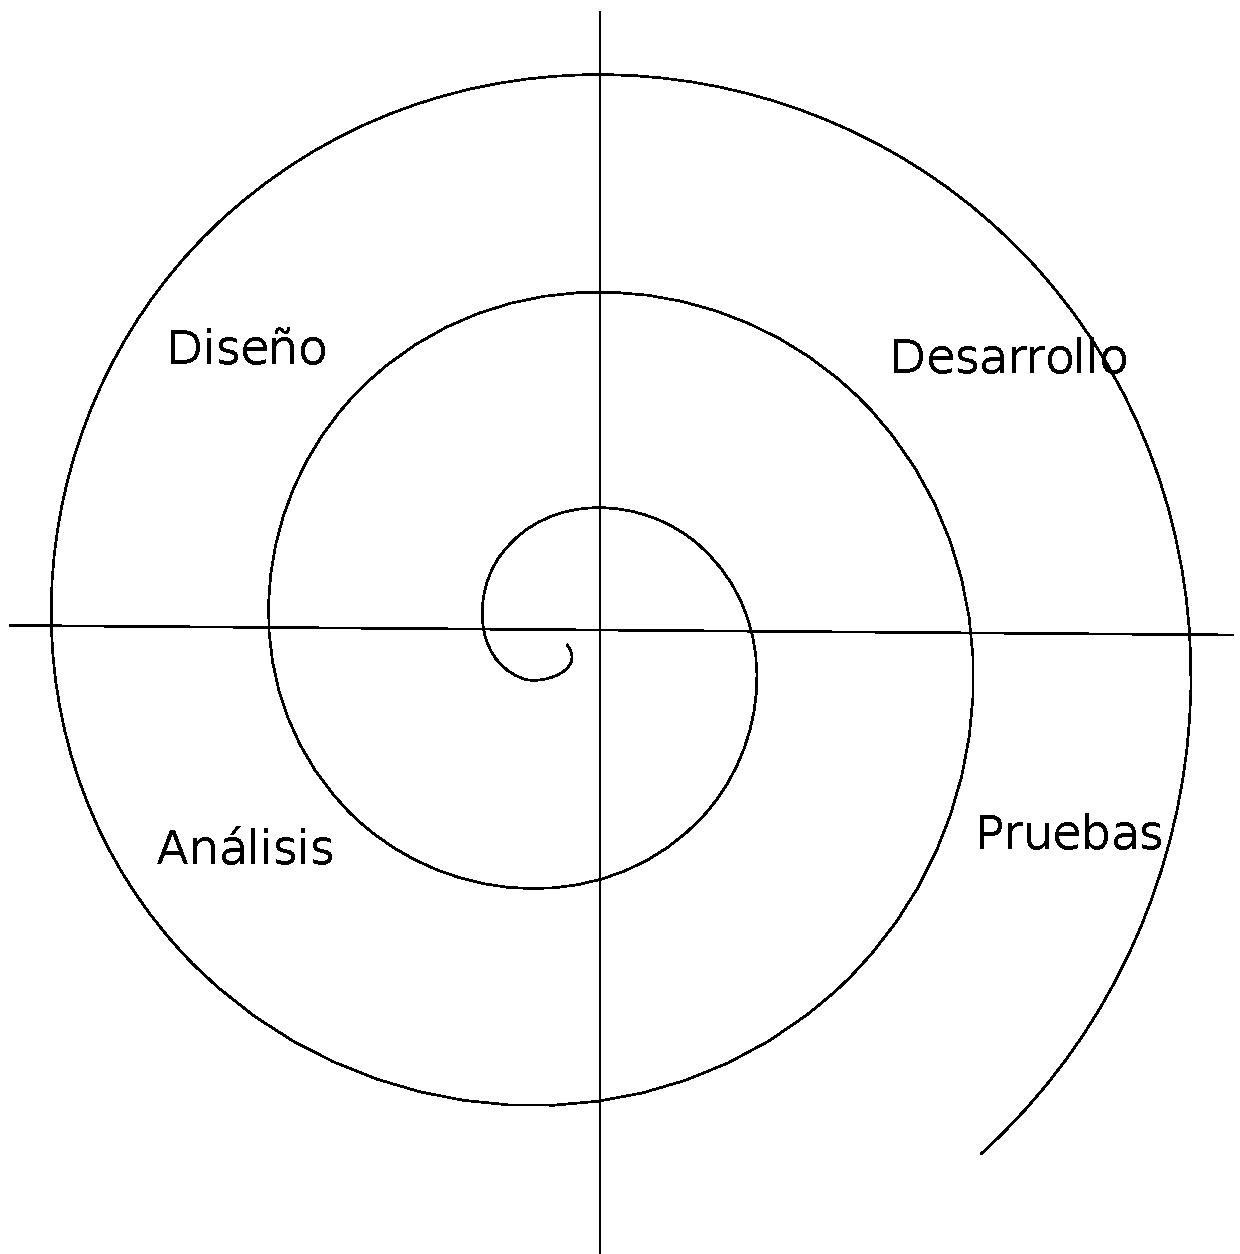
\includegraphics[scale=.4]{espiral.pdf} 
\end{center}
\caption[Metodología en espiral]{Metodología utilizada en jBomb fue en base a un espiral de 4 etapas.}
\end{figure}

\begin{description}
\item[Análisis] Antes de trabajar en la idea se hacía un breve análisis sobre qué y cómo sería implementada la idea y esta etapa era llevada a cabo sólo por el desarrollador a cargo. Si la nueva funcionalidad ameritaba que participaran ambos integrantes, se hacía una pequeña reunion para discutir el tema.
\item[Diseño] El diseño era la forma gráfica de cómo interactuaban los nuevos componentes con los ya desarrollados. Esta etapa fue la que más ayuda brindaba porque se podía ver de manera gráfica todo el análisis previo y podía ser mejor entendido por ambos desarrolladores.
\item[Desarrollo] En esta etapa se implementaba en código todas las funcionalidades, fue la etapa en la cual se invirtió más tiempo por todas las ideas y nuevas funciones del juego.
\item[Pruebas] Una vez finalizada todo el desarrollo, el código era probado para que éste hiciera lo que su idea original planteaba. Por lo general hubieron muy pocas veces en las que no se tuvo que incurrir en unos cambios, de hecho la mayoría de éstos eran para mejorar en rendimiento o un comportamiento extraño, luego se volvían a hacer pruebas sobre los últimos cambios. Debido a toda esta retroalimentación se dice que el proyecto avanza en espiral.
\end{description}
Estas cuatro etapas fueron realizadas por todas y cada una de las funciones esperadas en el juego. Esta forma de trabajo se mantuvo desde el inicio hasta el final del proyecto y su utilización fue muy exitosa, para ello fue necesario tomar un poco de ambas metodologías nombradas antes y añadirles lo necesario para que el equipo pudiese sobrellevar bien el proyecto.

El equipo principal de desarrollo fue conformado por dos desarrolladores y un diseñador que apoyó en assets de imágenes y logos, así como la publicación y publicidad del juego. Otro integrante hizo su aporte en la música de fondo del juego.
Los nombres de los integrantes son:
\begin{itemize}
\item Rodrigo Villablanca (Desarrollador)
\item Diego Villablanca (Desarrollador)
\item Fernando de la Cerda (Diseñador)
\item Ricardo Reyes (Técnico en sonido)
\end{itemize}
\chapter{Desarrollo de jBomb}
Anteriormente ya se ha dicho de qué trata el juego, qué herramientas fueron utilizadas en su desarrollo, cuáles son sus características y qué metodología se abordó para gestionar el proyecto de una manera exitosa.\\
En este capítulo y el siguiente se entrará en aspectos mucho más técnicos y que tienen que ver con la etapa más importante del proyecto, el proceso de desarrollo.

\section{Estructura}
Muchos proyectos a la hora de ser desarrollados adoptan diversas formas en la que se distribuye el software. Por lo general se puede distribuir a través de un único archivo ejecutable, o bien a través de un conjunto de ellos, un archivo de instalación o un script de arranque. En general, existen diversas formas de hacerlo y las anteriores mencionadas son las más comunes. 

jBomb se distribuye a través de múltiples archivos que corresponden a las librerías utilizadas y al propio juego. Cuatro archivos principales corresponden al producto desarrollado que forman una parte del juego, un directorio con todas las librerías utilizadas y nombradas en los capítulos anteriores, y finalmente se crean un par de archivos más que corresponden a las librerías nativas de cada plataforma.

\begin{figure}[!hbp]
\begin{center}
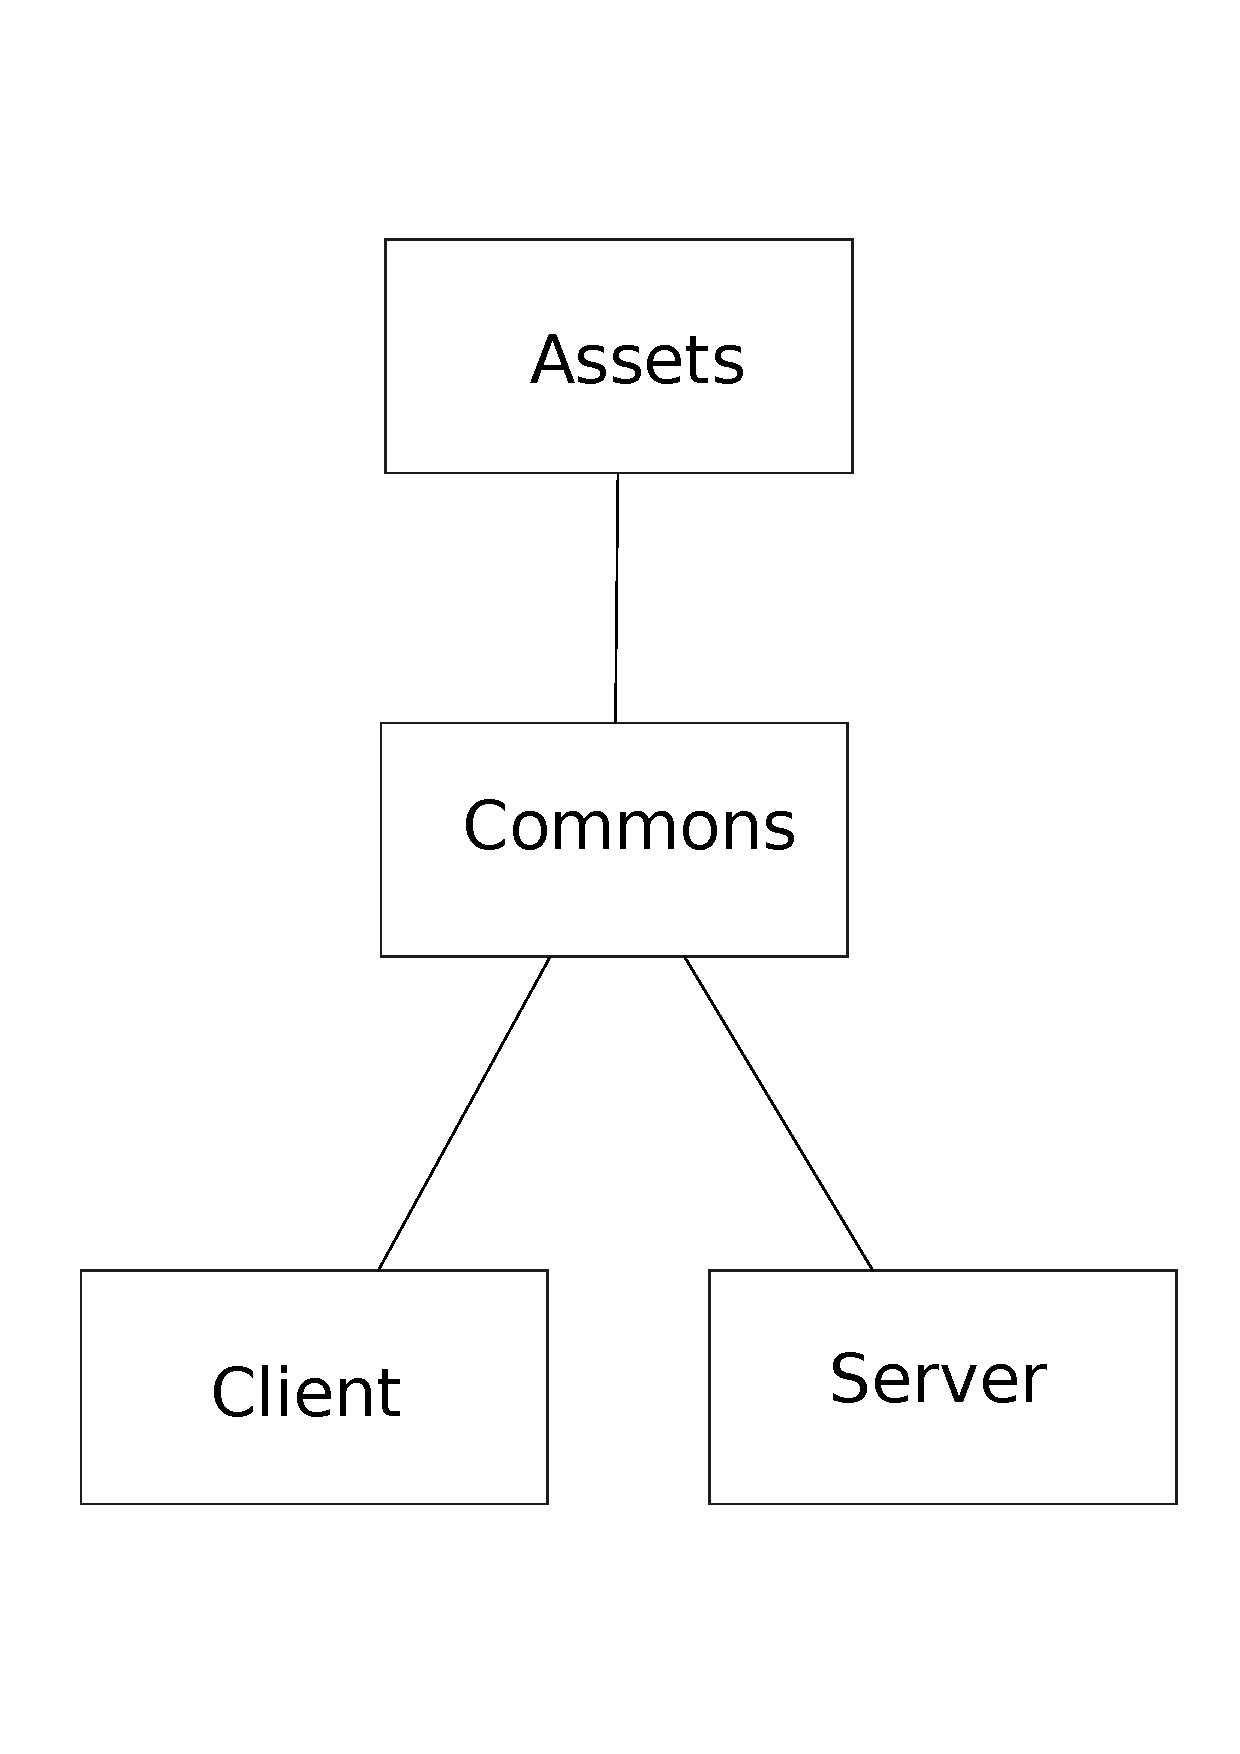
\includegraphics[scale=0.4]{estructura.pdf}
\caption[Estructura jBomb]{Estructura de jBomb}
\end{center} 
\end{figure}

Los cuatro archivos principales definen la estructura en la que se distribuye el juego, éstos son:
\begin{description}
\item[assets.jar] Este archivo almacena todas los assets de jBomb tales como imágenes, texturas y sonidos. Todos estos recursos son posteriormente utilizados por los demás componentes del juego.
\item[commons.jar] Este archivo contiene toda la lógica común que existe entre el cliente y el servidor. La mayor parte de los componentes más importantes se definen en este archivo y luego los otros archivos proporcionan únicamente las diferencias necesarias para poder ejecutarse.
\item[client.jar] Este archivo almacena toda la lógica del usuario del juego es aquí donde el usuario se identifica como tal. Si el usuario desea jugar, éste es el archivo mandatorio para poder hacerlo.
\item[server.jar] Finalmente el servidor proporciona toda la lógica necesaria para que los jugadores puedan conectarse entre sí. Generalmente este archivo es ejecutado en un ordenador con mayor capacidad y debe ser ejecutado por el administrador del juego para que pueda establecer algunas opciones al iniciarlo.
\end{description}
\section{Módulo de Assets}
Como se dijo anteriormente los assets de cualquier juego corresponden a todos los recursos utilizados por éste para poder hacer uso de ellos. Estos assets son de diversos tipos y los más comunes son:
\begin{description}
\item[Modelos] Los modelos por lo general corresponden a objetos específicos dentro de un videojuego, por ejemplo, personas, vehículos, maquinarias, animales, cosas, etc. Los modelos facilitan el desarrollo de los videojuegos porque independizan la creación de estos recursos necesarios, los hace más portables y disminuyen la tarea para los desarrolladores, dejándoselas a los diseñadores.
\item[Imágenes] Las imágenes son utilizadas en todos los juegos, como por ejemplo para el logo del juego.
\item[Texturas] Las texturas no son muy diferentes de las imágenes, de hecho son imágenes pero que poseen componentes adicionales que permiten aumentar la velocidad de renderización de éstas. La diferencia está en la funcionalidad que proveen, mientras las imágenes sirven como para ilustrar algo, las texturas tienen patrones conocidos que hacen que al colocarlas juntas se forme una gran imágen, por ejemplo para las murallas en vez de utilizar una gran imágen, se utiliza una sola textura que represente el ladrillo de la muralla, de manera que al hacer un arrastre de ella en sentido vertical y horizontal se forme la imágen de la muralla. Esto mejora el rendimiento del juego  \cite{JMONKEY}.
\item[Sonidos] Los sonidos son utilizados nada más que para el propósito que fueron hechos, para los videojuegos pueden utilizarse al desencadenar ciertas acciones, como por ejemplo al realizar un disparo o al caer desde cierto lugar, al rugir un animal o como sonido ambiental del bosque.
\end{description}
Por lo general esos son los más comunes pero también existen algunos especializados, en este caso JMonkeyEngine ofrece algunos tales como:
\begin{itemize}
\item Animaciones
\item Mallas geométricas
\item Escenas
\item Materiales
\item Shaders
\end{itemize}
jBomb no hace utilización de estos assets especializados sino que utiliza los más comunes y actualmente posee sonidos, texturas e imágenes.
\subsection{Sonidos}
En jBomb se utilizan al menos 2 tipos de sonidos, éstos son:
\begin{description}
\item[Background] Se utiliza como sonido de trasfondo durante la ejecución del juego. Anteriormente se dijo que el videojuego estaba inspirado en el espacio y por tanto el juego es acompañado por un estilo de música Electrónica. El sonido comienza cuando se inicia la cuenta regresiva del comienzo de la ronda. La música fue hecha especialmente para jBomb, el autor es Ricardo Reyes, técnico en sonido.
\item[Instancia] El sonido de este tipo se desencadena luego de alguna acción realizada por el jugador. Para jBomb, esto se refleja al lanzar bombas y en la explosión de éstas.
\end{description}
Cabe destacar que a pesar de ser recursos utilizados por el juego, son éstos los que finalmente le añaden mucho valor agregado al juego y que son fácilmente perceptible por los jugadores. Se hace esta mención debido a que el proceso de desarrollo del videojuego es bastante costoso en términos de trabajo, y si el juego sólo contara con el resultado de este proceso tal vez no sería tan entretenido para el usuario, a pesar que el juego ofrece la misma funcionalidad. Los assets dan mucho valor agregado al juego y los usuarios se dan cuenta de ello, ésto puede ser determinante a la hora de decidir si volver a jugar el juego o no hacerlo.
\subsection{Imágenes} El juego hace utilización de imágenes para mantener informado al usuario. Dentro de toda la escena gráfica existen 2 tipos de nodos que permiten dibujar en la pantalla. Está el nodo raíz \cite{BEGINNERS} que se encarga de dibujar todo lo que pertenece a la acción del juego, como los jugadores, las bombas, el escenario y todo lo que está involucrado con la lógica y objetivo del juego. Pero para llevar a cabo el estado actual del juego es necesario mostrar la información de éste, y para esto está el nodo de Interfaces Gráficas de Usuario (GUI Node).

Este nodo se encarga de dibujar en la pantalla de una manera diferente al nodo raíz, principal diferencia es que lo que dibuja es generalmente en dos dimensiones y se utiliza generalmente para mostrar información \cite{BEGINNERS}. Todos los juegos tiene ciertas mecánicas de juego, por ejemplo para jBomb está la mecánica de juego que permite mantener al jugador con al menos 3 bombas disponibles para ser lanzadas cada cierto tiempo. Si el jugador lanza una bomba, es necesario que se le avise cuántas bombas les queda luego de haber hecho ese lanzamiento.  El GUI Node sirve para aquello y éste dibuja en la pantalla toda esta información.

GUI Node trabaja con imágenes para representar toda esta información relacionada con el estado actual del juego. Actualmente se encarga de dibujar la información relacionada con:
\begin{itemize}
\item Bombas: GUI Node mantiene la pantalla actualizada sobre la cantidad de bombas que puede lanzar el jugador a sus enemigos.
\item Tiempo: Se encarga de mostrar la duración actual seleccionada para la duración de las bombas antes de que exploten.
\item Energía: La pantalla se mantiene actualizada con toda la información relacionada con la energía que le queda a cada jugador que está participando en la ronda.
\item Información General: Tiene la función de mantener informado al jugador sobre lo que está sucediendo. De momento las funciones implementadas con esto hacen que informe sobre el ganador del juego, los perdedores y la cuenta regresiva de la ronda. En la Figura \ref{infogeneral} se muestran algunas imágenes utilizadas en jBomb para mostrar información de propósito general.
\end{itemize}
\begin{figure}[!hbp]
\begin{center}

\includegraphics[scale=0.7]{images.pdf}
\caption[Utilización de imágenes en jBomb]{Imágenes utilizadas por GUI Node en jBomb, para mostrar información general}\label{infogeneral}
\end{center}
\end{figure}
Toda esta información es mostrada a través de imágenes que se encuentran en el archivo de assets. A pesar de que la mayoría de la información se presenta con imágenes y texto en 2D (dos dimensiones), GUI Node no sólo se limita a trabajar con este tipo de formatos, también posee la característica de poder mostrar objetos 3D (tres dimensiones) tales como modelos.
\subsection{Texturas}
Los assets más utilizados dentro de jBomb son lejos las texturas. jBomb no hace utilización de modelos y por tanto la mayoría de la escena gráfica está compuesta por figuras geométricas que forman todo el escenario, entre ellos los personajes (que son simples esferas movíendose), las paredes y vidrios, las bombas, etc.

Es por esto que al ser figuras geométricas es necesario pintarlas o establecer en ellas texturas que les permitan verse dentro de la escena gráfica. Por este motivo existen diversas texturas que son utilizadas por el juego. Actualmente las texturas que hay son para las cajas, figurás básicas que forman toda la escena, jugadores, cielo, bombas, vidrios y efectos de explosiones.

En la Figura \ref{textureslabel} se muestran algunas texturas utilizadas por jBomb.
\begin{figure}
\begin{center}
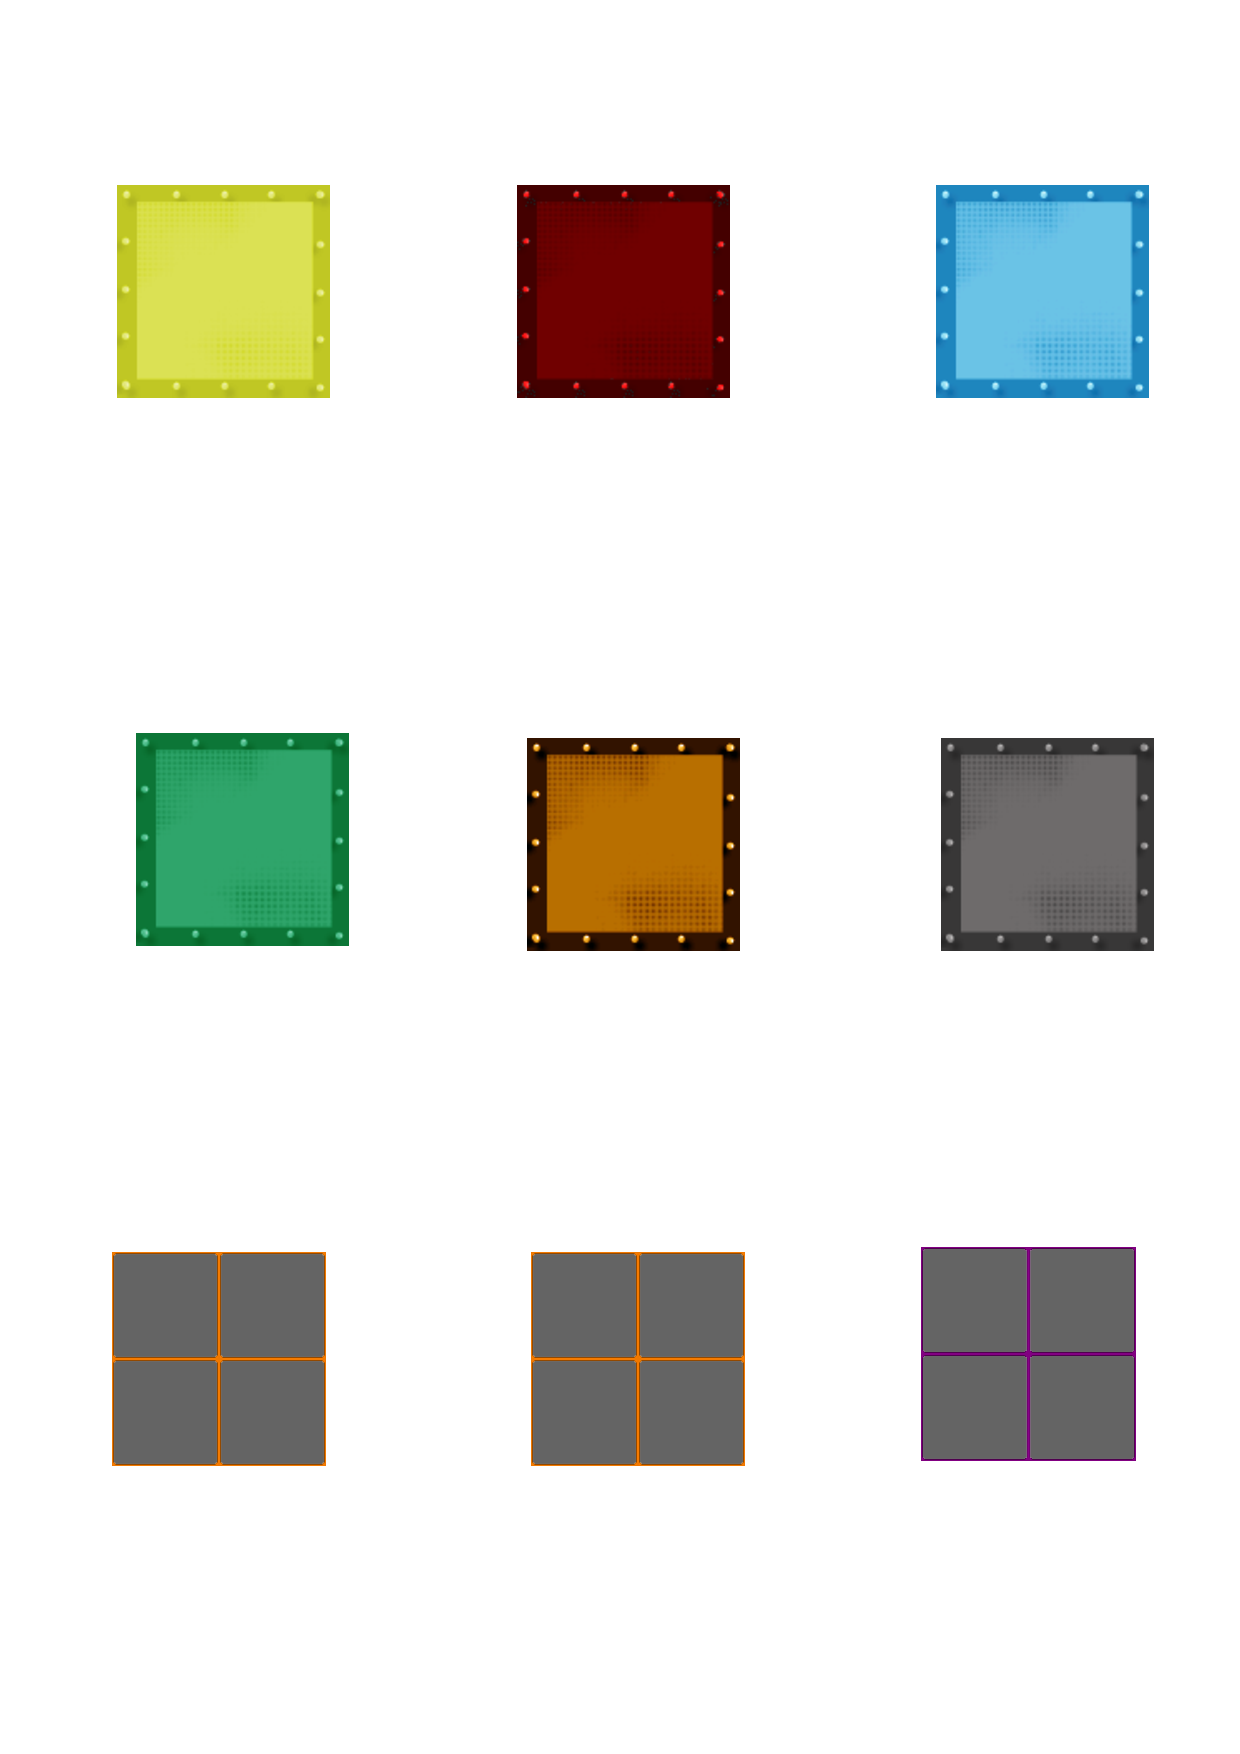
\includegraphics[scale=0.7]{textures.pdf} 
\end{center}
\caption[Utilización de texturas en jBomb]{Texturas utilizadas en jBomb, para ser utilizadas en objetos que forman la escenografía}\label{textureslabel}
\end{figure}

Las texturas permiten fácilmente pintar estas figuras con un ahorro considerable de recursos dado que la textura se repite hacia arriba y abajo, hacia los lados y también sobre el eje Z del espacio 3D.
\section{Módulo Común}
Este módulo es el más importante porque es el que provee la funcionalidad base para los demás módulos y en éste se concentra casi la mayoría del código que define el comportamiento del juego y sus componentes tales como controles de comportamiento, estados de aplicación, efectos, juego núcleo y contextos, entre otras cosas.

Cabe mencionar que aquí se detallarán sólo los componentes más importantes que se encuentran en este módulo dado que la cantidad de componentes que se encuentran en él son demasiados y se salen del foco de estudio de este capítulo. Los componentes principales se puden agrupar de la siguiente manera:
\begin{description}
\item[Estados de aplicación] Permiten a una aplicación agrupar ciertas características que tienen sentido sólo dentro de una determinado contexto \cite{BEGINNERS}. Por ejemplo cuando un jugador decide poner en estado de pausa un juego, éste presiona el botón que desencadena dicha acción y posteriormente el juego detiene su ejecución. Este estado en pausa es un estado de aplicación.
\item[Controles] Los controles permiten a un objeto en el juego tener un comportamiento definido. Esto permite que el comportamiento pueda ser más modularizado y dividido en varios controles, y posteriormente pueden ser agregados al objeto para definir todos sus comportamientos \cite{BEGINNERS}.
\item[Efectos] jBomb hace utilización de varios efectos visuales que son lanzados cuando ocurren ciertos sucesos, como por ejemplo cuando una bomba estalla o cuando un jugador pierde en la ronda\cite{BEGINNERS}.
\item[Juego Base] Aquí se define la mayoría de el contrato que debe cumplir el juego en sus dos modalidades, dejándole a las instancias proveer el comportamiento adecuado para esa interfaz. De aquí heredan el cliente y el servidor.
\item[Contexto] El juego utiliza un contexto en donde almacena algunas de las variables más utilizadas por los módulos, esto con el fin de proveer facilidad de acceso a estas variables.
\end{description}
\subsection{Estados de aplicación} Como se dijo anteriormente un estado de aplicación permite al jugador entrar en varios estados del juego, el caso más común es el estado de pausa. Otro estado de aplicación que es conocido es el de opciones, en el cual al estar dentro de él el juego pareciera estar en estado de pausa y los controles (tanto Joystick como teclado o cualquier otro dispositivo) sólo responden para gatillar acciones que afectan al panel de opciones.

Este es el objetivo principal de estos estados, agrupar ciertos componentes tales como controles, geometrías y objetos de juego para así habilitar y deshabilitar ciertas opciones de todos estos componentes. Dentro de jBomb se definieron varios estados de aplicación, \textit{CounterAppState}, \textit{WaitingAppState}, \textit{ServerManager}, \textit{ClientManager} sin embargo existen dos que son más importantes y juegan un papel crucial en el juego, éstos son \textit{RunningAppState} y \textit{AbstractManager}.
\subsubsection{RunningAppState}
\textit{RunningAppState} es un estado de aplicación y componente principal del juego el cual se inicia cuando el servidor lo decide. Este estado de aplicaión se mantiene activo durante toda la ejecución de la ronda actual. Sin embargo en este módulo sólo se define como una interfaz que marca a la aplicación para que posteriormente pueda ser implementada por el cliente o por el servidor.

El estado inicia cuando termina otro estado de aplicación que se encarga de realizar un conteo regresivo antes de iniciar la nueva ronda, y termina cuando la ronda es ganada por algún jugador. Básicamente este estado tiene diversas funciones dependiendo del contexto en el que se esté ejecutando, así para el servidor se ejecutan acciones totalmente distintas de las que se ejecuta en el cliente.

Dentro del servidor el componente que se encarga de dar la funcionalidad y extender de \textit{RunningAppState} es un componente llamado \textit{RunningServerAppState} y las acciones que se realizan son las siguientes:
\begin{description}
\item[Coordinación de bombas] El componente se encarga de llevar a cabo toda la coordinación de las bombas que son lanzadas por los jugadorers de la ronda Coordinar se entiende por llevar un seguimiento de todas las bombas e informarles a los demás clientes de la posición actual de dicha bomba, además se encarga de avisar a todos sobre cuándo es el momento en que la bomba explotará, de esa manera todos los clientes verán en casi el mismo instante la explosión de la bomba.
\item[Coordinación de elevadores] Dentro del juego existen unos elevadores que permiten a los jugadores subir más niveles en la etapa, esto es parte del juego. La dificultad está en que estos elevadores deben ser vistos por todos los jugadores desde distintos puntos de vista por lo que se debe llevar una coordinación de éstos para que todos vean el mismo elevador en una posición determinada pero desde distintas perspectivas, toda esta coordinación también es llevada a cabo por \textit{RunningServerAppState}.
\end{description}
En las cajas de código \ref{lst1} y \ref{lst2} se muestran un par de fragmentos de código correspondientes a la funcionalidad de \textit{RunningServerAppState}.
\begin{codigo}
\begin{lstlisting}[language=Java,frame=single,basicstyle=\scriptsize]
private void coordinateBombs() {
        Object o = null;
        GrandBomb gb = null;
        for (long l : JBombContext.MANAGER.keySet()) {
            o = JBombContext.MANAGER.getPhysicObject(l);
            if (o instanceof GrandBomb) {
                gb = (GrandBomb) o;
                CoordinateBombMessage cbm = new CoordinateBombMessage(l,
                        gb.getSpatial().getControl(RigidBodyControl.class));
                ServerContext.SERVER.broadcast(cbm);
            }
        }
    }
\end{lstlisting}
\caption{Método de coordinación de bombas}
\label{lst1}
\end{codigo}
\newpage
\begin{codigo}
\begin{lstlisting}[language=Java,frame=single,basicstyle=\scriptsize]
private void coordinateElevators() {
        synchronized (JBombContext.MANAGER.getPhysicsObjects()) {
            for (long l : JBombContext.MANAGER.keySet()) {
                Object o = JBombContext.MANAGER.getPhysicObject(l);
                if (o instanceof Elevator) {
                    Elevator e = (Elevator) o;
                    Vector3f location = e.getGeometry()
                    	.getControl(RigidBodyControl.class)
                    	.getPhysicsLocation();
                    ServerContext.SERVER.broadcast(
                    	new ElevatorMovesMessage(e.getId(), location));
                }
            }
        }
    }
\end{lstlisting}
\caption{Método de coordinación de elevadores}
\label{lst2}
\end{codigo}
En el caso del cliente las acciones que se realizan son muy diferentes y van en directa relación sólo con la perspectiva del usuario ya que los otros jugadores son manejados por el servidor (desde el punto de vista del usuario). La implementación del cliente para \textit{RunningAppState} se llama \textit{RunningClientAppState} y las funciones llevadas a cabo son las siguientes:
\begin{description}
\item[Movimiento de jugador] Esta función se encarga de posicionar la cámara a la posición actual del jugador según las teclas presionadas por el usuario y tambíen tiene que avisar sobre esa posición al servidor, para que éste último pueda finalmente avisarles a todos los demás jugadores sobre la posición actual del jugador local.
\item[Listening de bombas] Esta función se encarga de hacer que el sonido causado por el lanzamiento y explosiones de bombas sea relativo a la posición actual del jugador. Esto hace que el jugador escuche una bomba según donde están posicionadas, es decir que si la bomba estaba lejos del jugador el sonido percibido será menor al que causaría la explosión de una bomba que está ubicada más cerca del jugador. Esto logra una sensación de realismo no sólo a nivel visual sino a nivel auditivo.
\item[Recarga de bombas] Esta funcionalidad es la que se encarga de llevar el conteo de las bombas que puede lanzar el jugador en cada instante, además de el tiempo de recuperación que tiene cada una de las bomba. En una mecánica de juego mencionada antes se dijo que el tiempo de recuperación de cada bomba lanzada era de 5 segundos, y de esto jústamente se encarga \textit{RunningClientAppState}.
\item[Carga de interfaz] La carga de interfaz es la función que está constantemente refrescando la pantalla de información a través del GUI Node. Esto quiere decir que toda la información relativa a la energía de los jugadores, a las bombas y al tiempo de explosión de cada una es tarea de \textit{RunningClientAppState}.
\end{description}
En la caja de código \ref{lst3} se muestra un fragmento que hace utilización de las funciones definidas arriba. Este fragmento pertenece a \textit{RunningClientAppState}.
\begin{codigo}
\begin{lstlisting}[language=Java,frame=single,basicstyle=\scriptsize]
    @Override
    public void update(float tpf) {
        moveCam(tpf);
        hearingSounds();
        reloadBombs(tpf);
        loadInterface();
    }
\end{lstlisting}
\caption{Método de actualización de estado para \textit{RunningClientAppState}}
\label{lst3}
\end{codigo}
\subsubsection{AbstractManager}
\textit{AbstractManager} es considerada una pieza fundamental para jBomb y es el componente más importante en la gestión de paso de mensajes en red. \textit{AbstractManager} controla toda la información relativa a objetos de deben ser identificados de alguna manera para que puedan ser manejados de la misma forma en todos los clientes. 

Para esta tarea \textit{AbstractManager} tiene un componente llamado \textit{IDRepository} que es el encargado de llevar los registros o identificadores ocupados por los objetos y se encarga de liberar o reservar estos identificadores, éste puede verse como una base de datos con todo el estado de los identificadores de estos objetos. 

Este \textit{IDRepository} mantiene en memoria sólo los ID's que tiene reservados, y una vez que son liberados se mantienen en memoria para una posterior reserva, de esta manera el uso de memoria RAM sólo aumenta cuando la cantidad de objetos a ser identificados supera a la cantidad de ID's disponibles en memoria.

Básicamente \textit{AbstractManager} es el núcleo de todo el paso de información entre los usuarios y esta información puede contener a la posición de los jugadores, a la posición de los elevadores y a la posición de las bombas

\textit{AbstractManager} actúa como dos componentes en uno. Basicamente tiene la capacidad de estar atento a ciertos mensajes que pueden ser enviados por los clientes. En segundo lugar actúa como un estado de aplicación que está constantemente aplicando las acciones asociadas a esos mensajes.

La velocidad con la que aplica esos mensajes es actualmente cuatro veces por segundo \cite{VALVE1}. Al ser la velocidad de aplicación de los mensajes menor a la velocidad con la que recibe los mensajes, es necesario que este almacene todos los mensajes en una cola, de manera que puedan ser aplicados una vez que llegue el momento de hacerlo.

El funcionamiento de \textit{AbstractManager} es muy similar en el servidor como en el cliente con la única diferencia de que además de aplicacar la accion asociada con los mensajes, en el lado del servidor se hace un reenvío de los mensajes a todos los otros jugadores, incluso en algunos casos el mensaje es reenviado a todos incluyendo al jugador que inició el mensaje.

Dado que la diferencia entre las implementaciones de \textit{AbstractManager} tanto en el servidor como en el cliente es bastante sutil en lo que respecta a qué, los resultados de la ejecución de los mensajes depende exclusivamente del mensaje que se está ejecutando.

Las cajas de código \ref{lst4} y \ref{lst5} ilustran el trabajo principal llevado a cabo por \textit{AbstractManager}, independiente de su implementación. Las funciones corresponden a su doble rol, tanto como Listener y como Estado de Aplicación.
\newpage
\begin{codigo}
\begin{lstlisting}[language=Java,frame=single,basicstyle=\scriptsize]
    @Override
    public void messageReceived(T source, Message m) {
        messageQueue.add((BasePhysicMessage) m);
    }
\end{lstlisting}
\caption{Métodos de listener de \textit{AbstractManager}}
\label{lst4}
\end{codigo}
\begin{codigo}
\begin{lstlisting}[language=Java,frame=single,basicstyle=\scriptsize]
    @Override
    public void update(float tpf) {
        time += tpf;
        Iterator<BasePhysicMessage> it = messageQueue.iterator();
        BasePhysicMessage message = null;
        if (time >= maxTime) {
            time = 0;
            while (it.hasNext()) {
                message = it.next();
                doOnUpdate(tpf, message);
                it.remove();
            }
        } else {
            while (it.hasNext()) {
                message = it.next();
                if (message instanceof CharacterMovesMessage || 
                message instanceof ElevatorMovesMessage) {
                    message.interpolate(time / maxTime);
                }
            }
        }
    }
\end{lstlisting}
\caption{Método de actualización de \textit{AbstractManager}}
\label{lst5}
\end{codigo}
Por ejemplo cuando el mensaje se trate de un mensaje con las posiciones de algún jugador, \textit{ServerManager} (la implementación de \textit{AbstractManager} en el módulo de servidor) será el encargado de realizar su ejecución, lo que se traduce en asignar las coordenadas de el jugador que está en el servidor con las posiciones que vienen en el mensaje, y posteriormente reenviar el mensaje a los demás clientes.

Una vez que el mensaje sea recibido por los jugadores, \textit{ClientManager} (la implementación de \textit{AbstractManager} en el módulo del cliente) será el encargado de asignar las coordenadas del jugador con la copia de dicho jugados en su cliente, de esta manera todos los jugadores pueden ver que el jugador se está moviendo desde un punto A a un punto B, pero como siempre desde distintas perspectivas.

Esta es la funcionalidad básica que provee \textit{AbstractManager} y acaba de ser resumida en los puntos más importantes, sin embargo esta pieza de software fue cuidadosamente diseñada porque está muy involucrada con la comunicación en red que hay entre los clientes y el servidor.
\subsection{Controles}
Los controles son componentes especiales que ayudan a separar todo el el comportamiento de alguna entidad en piezas completamente independientes y reutilizables \cite{BEGINNERS}. Con esto se tienen al menos 2 grandes beneficios, el primero es que se logra una mejor división del código, permite una mejor legibilidad y promueve el desarrollo ordenado. El segundo es que al quedar en un objeto encapsulado tal comportamiento, este puede ser fácilmente reutilizado y puede ser compartidos con múltiples instancias de un objeto a través de clonación.

En todos los motores de juegos existe una forma común de ejecutar su actualización, esto es a través de un ciclo de ejecución denominado \textit{Event Loop}. Dentro de este ciclo de eventos se realizan tareas como la verificación de entradas de usuario, la ejecución de inteligencia artificial en los Controles, el cálculo de físicas, la reproducción de sonidos y finalmente el dibujo de los gráficos.

Para delegar cierta porción de tiempo del \textit{Event Loop} al usuario, JMonkeyEngine proporciona un método llamado \textit{update()} que permite trabajar la lógica del juego \cite{BEGINNERS}. Dentro de este método por lo general va incluido todo el estado de la aplicación y de los objetos que participan en la escena. Estos objetos se denominan Instancias y por lo general se trata de personajes que son reelevantes en la historia del juego. Estas instancias tienen sus propias variables que definen todo su estado actual y por lo general son fácilmente reconocidas por los usuarios. 

En el método \textit{update()} se controla todo el comportamiento del juego y las instancias, pero a medida que éste va creciendo la mantención del software se hace más dificil de mantener. Para ello, se elaboraron dos formas de delegar esta tarea a componentes que pudieran ser reutilizables y que permitieran estructurar el código de una manera más ordenada. Uno de estos componentes son los estados de aplicación mencionados antes que se encargan jústamente de llevar un seguimiento del estado de la aplicación a través de múltiples estados de aplicación y así poder controlar el comportamiento general del juego.

El otro tipo de componente son los controles que están encargados de lo mismo que los estados de aplicación pero esta vez orientados a las instancias. En jBomb se utilizaron varios controladores ya implementados en JMonkeyEngine, pero otros fueron desarrollados a medida para Instancias tales como los elevadores, bombas y jugadores.

Los controladores incluidos en el módulo común son:
\begin{description}
\item[JBombAbstractControl] Para jBomb se diseñó este control que provee la funcionalidad básica para soportar la clonación de los controles. Esta funcionalidad es ampliamente utilizada porque existen muchas instancias que necesitan tener un comportamiento igual al de otras instancias, y para ello se utiliza la clonación. También podría resolverse este problema a través de nuevas instancias de los controles, pero esto no hace una copia exacta sobre el estado del control de otra Instancia.
\item[BaseControlExplosion] Este control se encarga de el comportamiento de la explosiones de las bombas. Su función es determinar en qué momento la explosión debe desaparecer del escenario para dejar de causar daño a los personajes.
\item[AbstractBombControl] Este control está encargado de iniciar la explosión según ciertos criterios. Los dos criterios que se usan para determinar si la bomba explota son, si ésta llega a su tiempo de expiración debe explotar inmediatamente o bien si ésta determina alguna colisión con alguna Instancia de Jugador, debe explotar inmediatamente. Este controlador actúa siempre antes que \textit{BaseControlExplosion}.
\item[ThrowBombControl] Este control se encarga de sincronizar la aplicación de fuerzas a las bombas con la velocidad de los ticks del motor de físicas. Esto sucede porque por lo general el motor de físicas trabaja a una velocidad de 60 [Ticks/seg] constante, y hay ocaciones en las que el motor de renderizado está trabajando a una velocidad mayor y por esa razón la aplicación de fuerzas físicas deben postergarse para cuando sea el momento correcto, de lo contrario se obtienen resultados incorrectos.
\end{description}
En la caja de código \ref{lst6} se ilustra un fragmento de código del Control \textit{BaseControlExplosion}.
\begin{codigo}
\begin{lstlisting}[language=Java,frame=single,basicstyle=\scriptsize]
	package jbomb.common.controls;
	
	import com.jme3.renderer.RenderManager;
	import com.jme3.renderer.ViewPort;
	import com.jme3.scene.control.Control;
	import jbomb.common.effects.api.Explosion;
	
	public class BaseControlExplosion extends JBombAbstractControl {
	    
	    private float time;
	    private Explosion explosion;
	
	    @Override
	    protected Control newInstanceOfMe() {
	        return new BaseControlExplosion();
	    }
	
	    @Override
	    protected void controlUpdate(float tpf) {
	        if(time >= explosion.getTimeForDie())
	            explosion.stop();
	        else
	            time += tpf;
	    }
	
	    @Override
	    protected void controlRender(RenderManager rm, ViewPort vp) {}
	    
	    public void setExplosion(Explosion explosion) {
	        this.explosion = explosion;
	    }
	}
\end{lstlisting}
\caption{Clase \textit{BaseControlExplosion}}
\label{lst6}
\end{codigo}
\subsection{Efectos}
jBomb se puede clasificar como un juego de acción en tiempo real y para ello utiliza una variedad de efectos especiales que hacen que el juego sea más atractivo.

El juego contiene todo un contrato sobre qué hacen estos efectos a través de una Interfaz llamada \textit{Explosion} que define cómo se comporta el efecto. Existen diversas implementaciones de éstos y todas están relacionadas a dos momentos en que son utilizadas en el juego, cuando una bomba explota y cuando un jugador pierde.

En la Figura \ref{apilabel} se muestra un diagrama que componen todas las explosiones en jBomb.
La API define al menos 6 puntos con los que todo efecto debería cumplir, se muestran en la cada de código \ref{lst7}.
\begin{codigo}
\begin{lstlisting}[language=Java,frame=single,basicstyle=\scriptsize]
	package jbomb.common.effects.api;

	import com.jme3.math.Vector3f;
	import com.jme3.scene.Geometry;
	
	public interface Explosion {
	    
	    void config();
	    
	    void start();
	    
	    void stop();
	    
	    void setLocation(Vector3f location);
	    
	    float getTimeForDie();
	
	    Geometry getGeometry();
	}
\end{lstlisting}
\caption{API de \textit{Explosion}}
\label{lst7}
\end{codigo}

\begin{figure}
\begin{center}
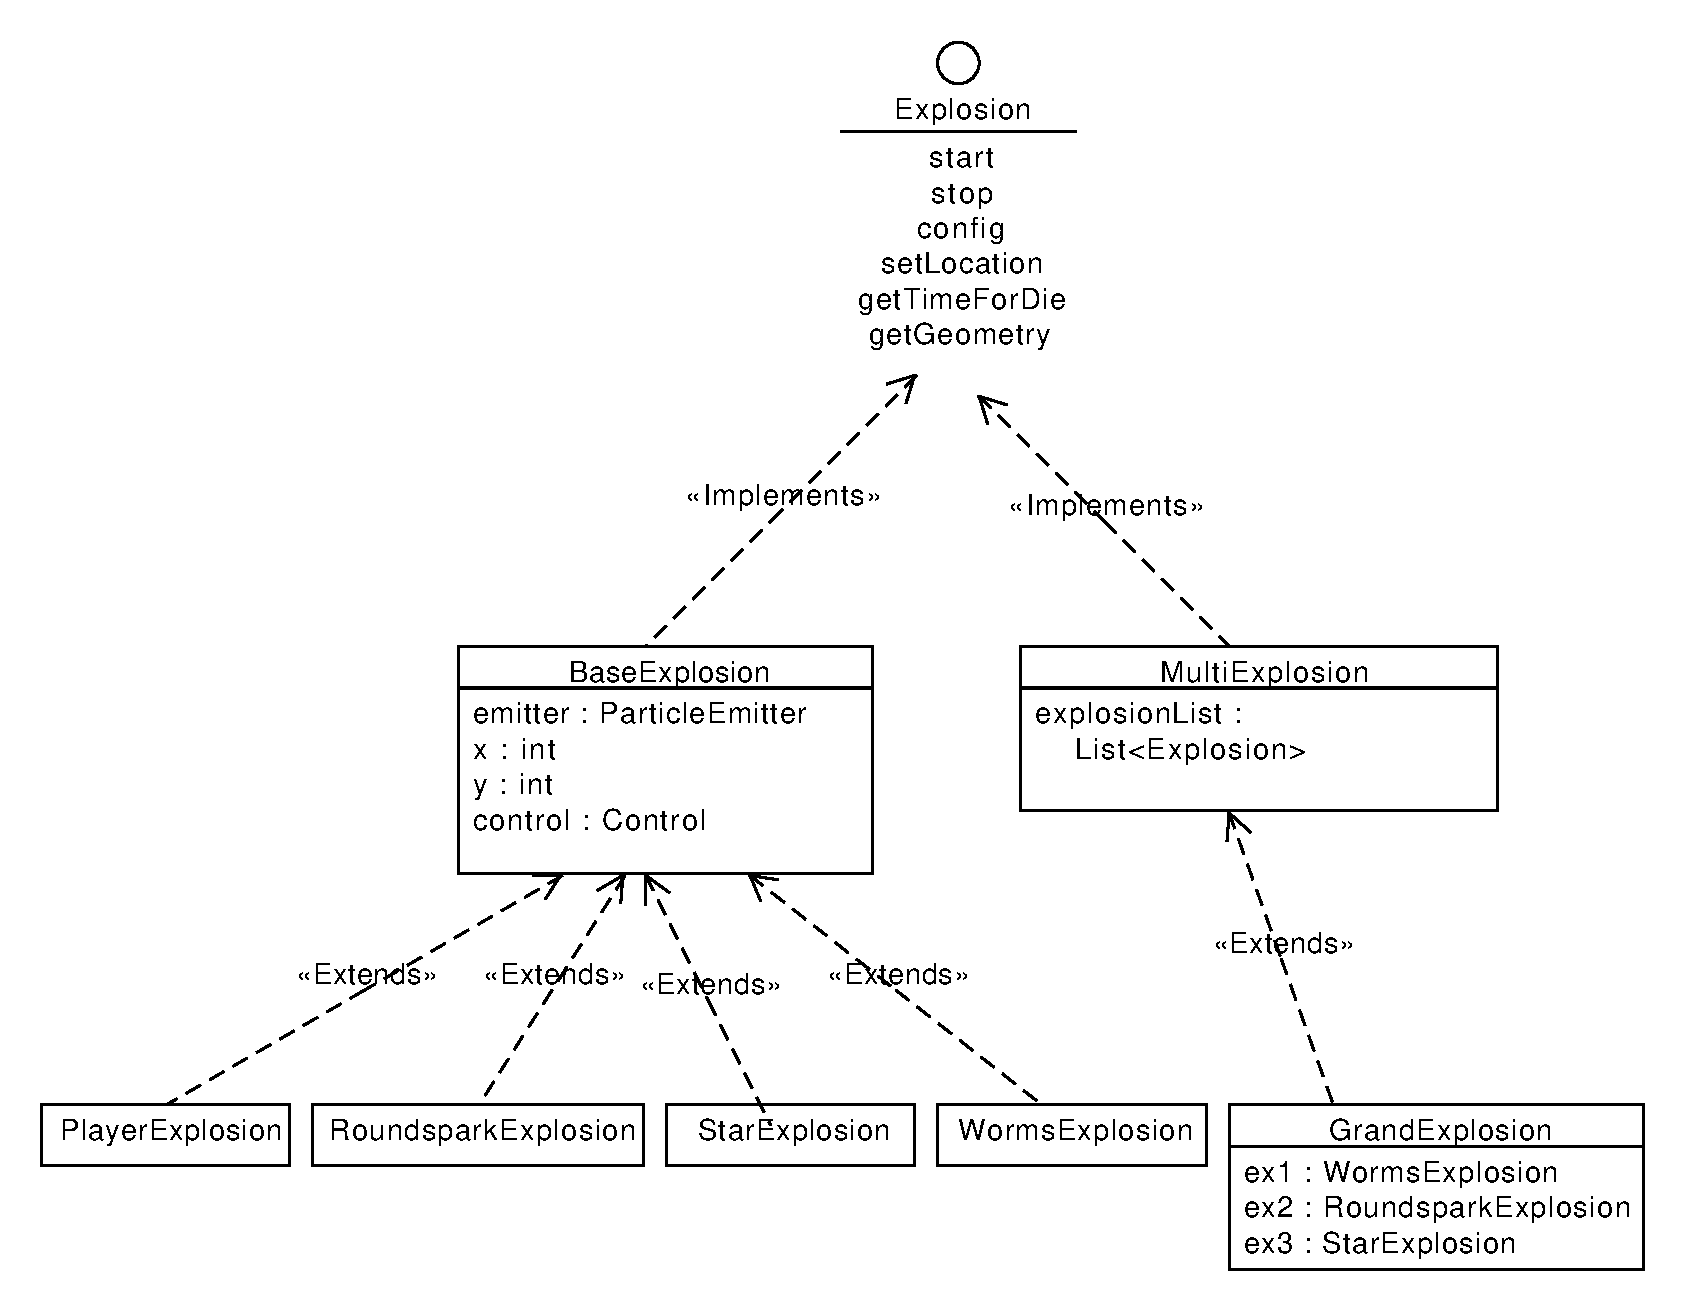
\includegraphics[scale=0.5]{explosions-diagram.pdf} 
\end{center}
\caption[Diagrama de clases - Explosion API]{Diagrama de clases para la API de explosiones}
\label{apilabel}
\end{figure}

El primer método es la configuración del efecto que permitirá controlar su tamaño deseado, establecerá la dispersión del efecto, las velocidades con las que aparecen y desaparecen, el estado de ser afectado por la gravedad, la dirección de la fuerza de gravedad, los colores que participan, etc. En este punto se hace una configuración completa del efecto para que este tenga la apariencia deseada y el método asociado para esto es \textit{config()}.

También se definen dos métodos que están vinculados con el inicio y término del efecto, éstos son \textit{start()} y \textit{stop()} respectivamente, ambos son llamados justo en el momento en que se desea que se realice tal acción.

Los demás métodos tienen que ver con la posición donde aparecerá el efecto, el tiempo de duración del efecto en escena y por último una referencia al objeto sobre el cuál tendrá acceso. Los métodos para esto son \textit{setLocation(Vector3f location)}, \textit{getTimeForDie()} y \textit{getGeometry()} respectivamente.

En cuanto a las implementaciones existen al menos 7 y se resumen en la siguiente tabla.
\begin{flushleft}
\begin{tabular}{|r|p{9cm}|}
\hline
\textbf{BaseExplosion} & Esta es la clase base para todas las demás explosiones. Se encarga de suministrar una implementación básica de la API y proporciona una configuración básica de la forma de la explosión.\\
\hline
\textbf{PlayerExplosion} & Esta es la explosión utilizada para simular la destrucción de un jugador. Esta explosión implementa la API a través de \textit{BaseBombExplosion}. \\
\hline
\textbf{RoundsparkExplosion} & Otra implementación que es utilizada en conjunto con otras para simular la explosión de las bombas. \\
\hline
\textbf{StarExplosion} & Esta explosión es una implementación de la API a través de \textit{BaseBombExplosion} y simula una explosión con forma de estrellas y es utilizada en conjunto con otras implementaciones para la simulación de la explosión de las bombas. \\
\hline
\textbf{WormsExplosion} & Es una explosión bien sutíl en donde muestra efectos parecidos a unos gusanos. Es utilizada junto a otras implementaciones para la explosión de bombas. \\
\hline
\textbf{MultiExplosion} & Esta clase es diferente a las demás implementaciones, ya que funciona como una explosión contenedora de otras explosiones. En ella se pueden agrupar cuantas explosiones se requieran y proporciona el comportamiento necesario para coordinar y configurar las explosiones. Esta clase es sólo una base y debe ser necesariamente implementada por otra para que sea ésta la que incluya las demás explosiones.\\
\hline
\textbf{GrandExplosion} & Esta es una implementación concreta de \textit{Multiexplosión} e incluye diversas implementaciones tales como \textit{WormsExplosion}, \textit{RoundsparkExplosion} y \textit{StarExplosion}. Esta implementación es la utilizada para simular la explosión de las bombas.\\
\hline
\end{tabular}
\end{flushleft}
\subsection{Juego Base}
El juego base es una clase llamada \textit{BaseGame} y es uno de los componentes principales del juego y uno de los más importantes en general. \textit{BaseGame} es la clase a partir de la cual se ramifican el cliente y el servidor, donde ellos son en última instancia los que definen el comportamiento final de la clase que marca justamente las diferencias entre éstos.

Tanto el servidor como el cliente deben manejar el mismo escenario, esto involucra el diseño de cajas espaciales, el fondo, el cubo pricipal, el espacio, los vidrios y toda la escenografía en general. Dado que esta es una característica compartida, esta queda delegada en \textit{BaseGame}. De hecho todo el código involucrado en el diseño de la escena está todo concentrado dentro de esta clase.

Aquí se define el cubo de vidrio principal, que es donde toda la acción ocurre, se definen los niveles (4 pisos en total), los elevadores, los cubos, vidrios, etc.

\textit{BaseGame} hace utilización de un estado de aplicación muy importante llamado \textit{BulletAppState}, el cual está encargado de dirigir todo el comportamiento de los componentes que están sujetos a la gravedad. Al comienzo de este capítulo se definió bien qué era un estado de aplicación y cuales eran sus funciones principales \cite{BEGINNERS}.

\textit{BaseGame} además utiliza un componente llamado \textit{AppSettings} que tiene la responsabilidad de mantener las configuraciones generales del juego como por ejemplo el tamaño de la ventana, la desición de mostrar o no opciones iniciales, título de la ventana del juego, etc.

jBomb trabaja en red local o internet y para llevar a cabo la comunicación sobre éstas es necesario transportar la información a través de clases especiales que puedan ser serializadas para así por transportarlas por la red. Estas clases se llaman Mensajes, y para hacer uso de estos es necesario primero registrar todos los mensajes a utilizar. Esta tarea es llevada a cabo también por \textit{BaseGame} dado que los mensajes utilizados son comunes para ambos componentes.

jBomb necesita compartir mucha información general que es accedida por muchas clases, o componentes a nivel más general, y para facilitar este proceso se hace uso de un contexto llamado \textit{JBombContext}. En las siguientes secciones se explicará en detalle qué información almacena dicho contexto, pero el componente encargado de inicializar esa información en el contexto es también \textit{BaseGame}.

Por último, en secciones anteriores se explicó todo sobre los estados de aplicación y entre ello se mencionó uno muy importante que gestiona muchos mensajes asociados con la identificación de objetos en la escena llamado \textit{AbstractManager}. A pesar que la implementación de este componente difiere sutílmente en el cliente y el servidor, la parte común es instanciada por \textit{BaseGame}.

Como se puede ver \textit{BaseGame} encapsula y gestiona la mayoría del comportamiento común que hay entre el cliente y el servidor, y para llevar esto a cabo hace utilización de los componentes principales antes mencionados. La Figura \ref{diagramlabel} se muestra un diagrama de clases de los principales componentes de jBomb.

\begin{figure}
\begin{center}
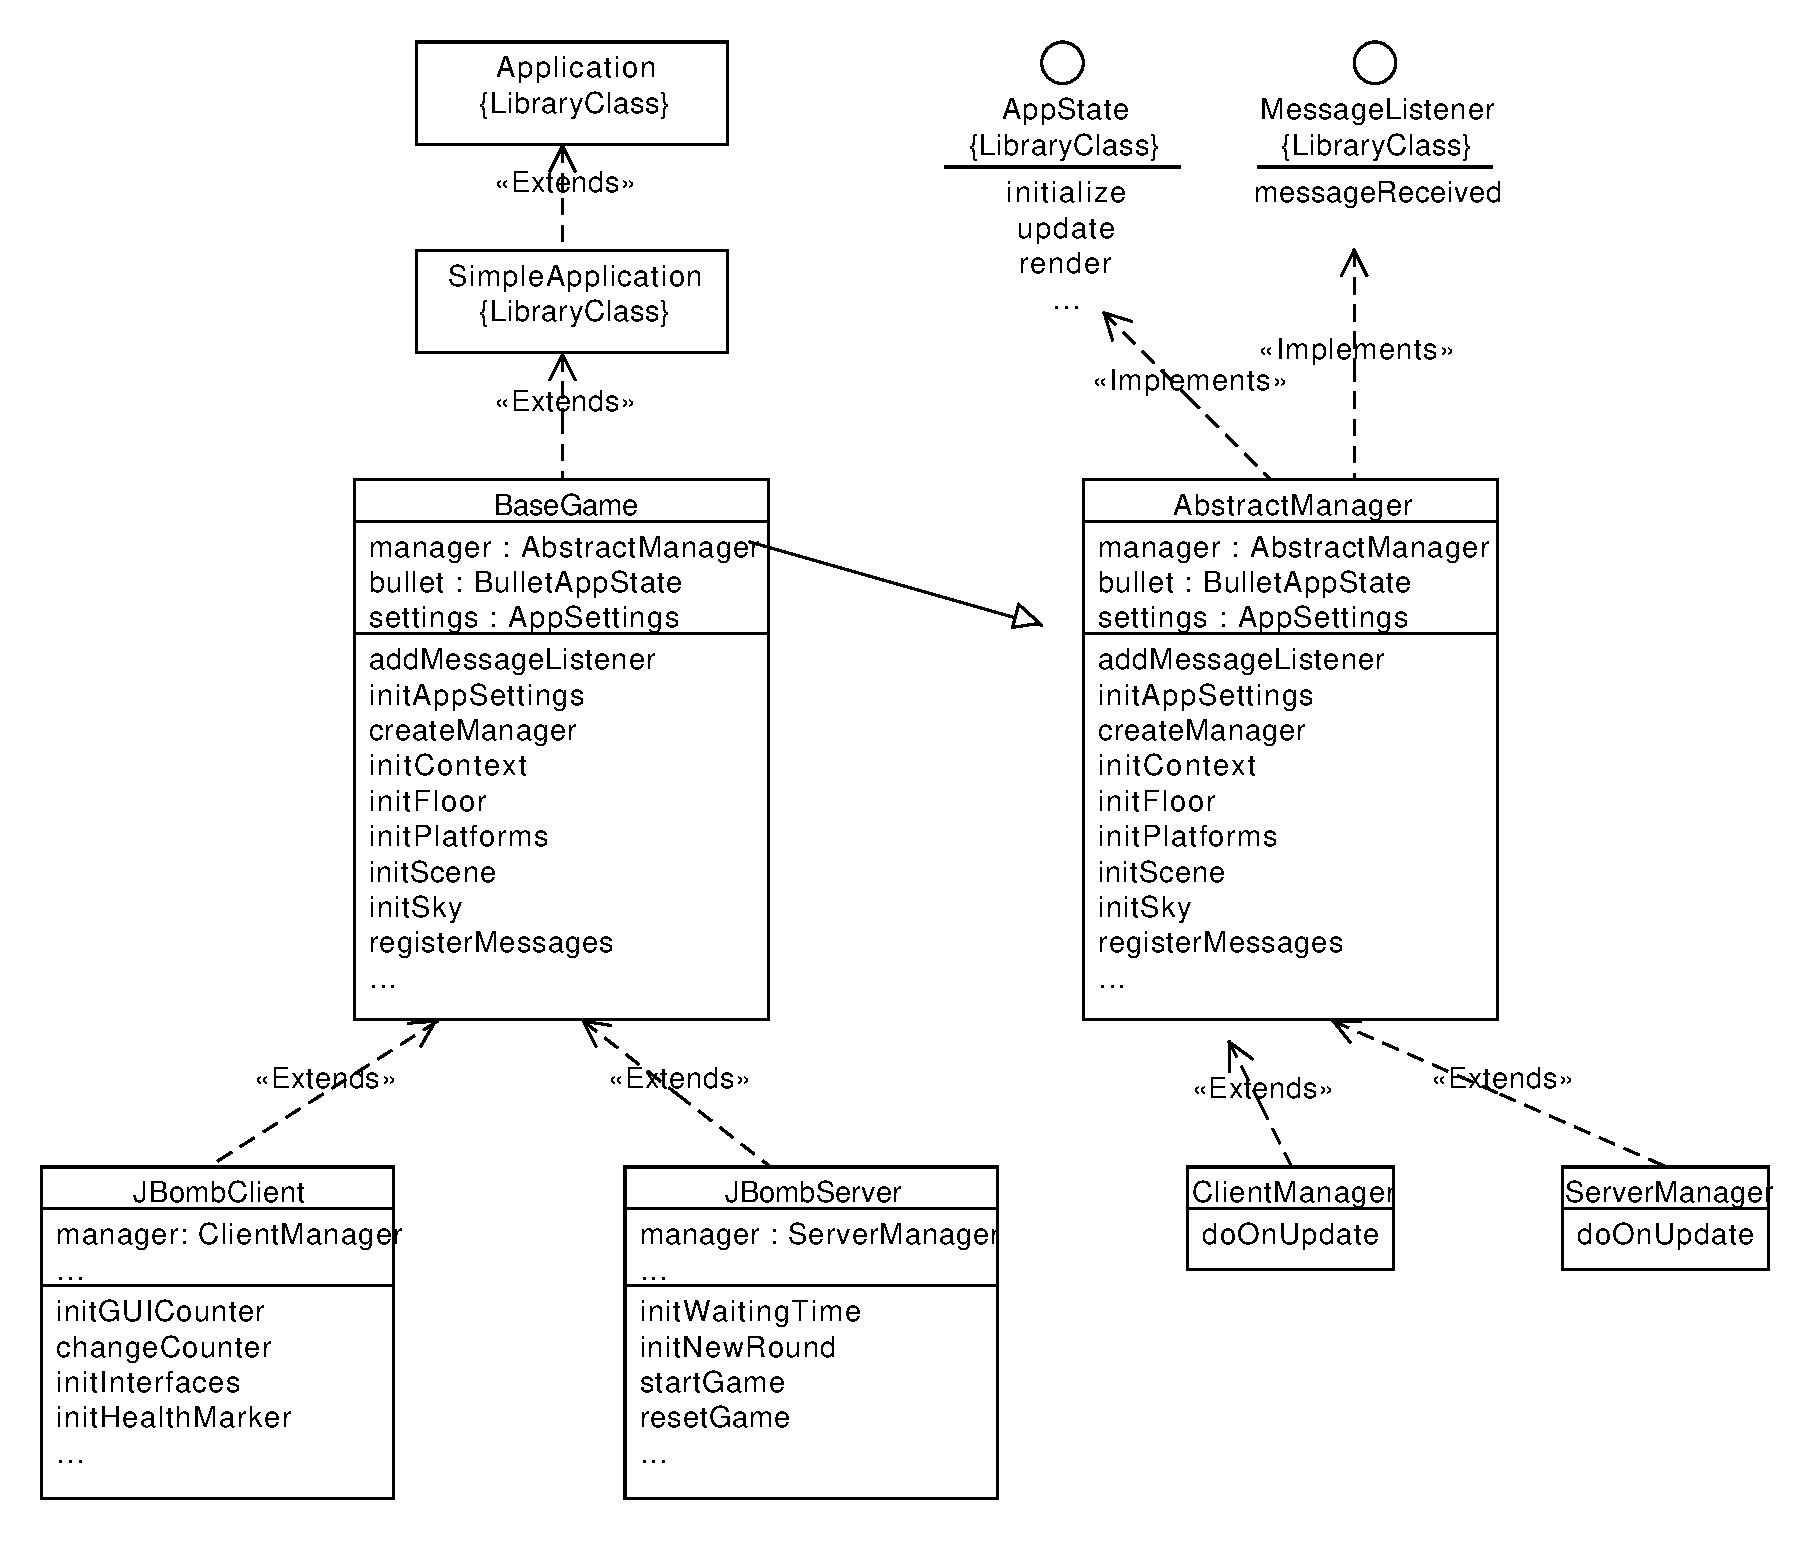
\includegraphics[scale=0.5]{diagram.pdf} 
\end{center}
\caption[Diagrama de clases - Componentes principales]{Diagrama de clases para los componentes principales de jBomb}
\label{diagramlabel}
\end{figure}

\subsection{Repositorio de ID's}
Como se dijo antes \textit{AbstractManager} cuenta con un repositorio que se encarga de identificar a todos los objetos dentro de la escena, solo aquellos que deben ser gestionados de igual forma en todos los clientes o jugadores conectados son identificados por \textit{AbstractManager} a través de este componente, el \textit{IDRepository}.

\textit{IDRepository} cuenta con un mapa que está compuesto por dos variables, un identificador y un valor que indica si dicho identificador está siendo ocupado o no lo está. Este mapa tiene una dimensión finita pero es lo suficientemente grande para ser utilizado como almacén de identificadores para los objetos de la escena.
\newpage
\textit{IDRepository} cuenta con métodos que permiten ocupar y liberar identificadores, permiten conocer la cantidad actual de identificadores en memoria, independiente de si están ocupados o no, y por último permite obtener el siguiente identificador libre para ser ocupado. Cabe destacar que \textit{IDRepository} reserva memoria sólo cuando el número de componentes a identificar es mayor que el número de identificadores disponibles. Cuando sucede esto, \textit{IDRepository} reserva memoria para crear un nuevo identificador o los que sean necesarios. Una vez que éstos son liberados \textit{IDRepository} los mantiene en memoria pero marcado en un estado de desocupado. Por lo general el número no supera los 30 identificadores.

\begin{figure}
\begin{center}
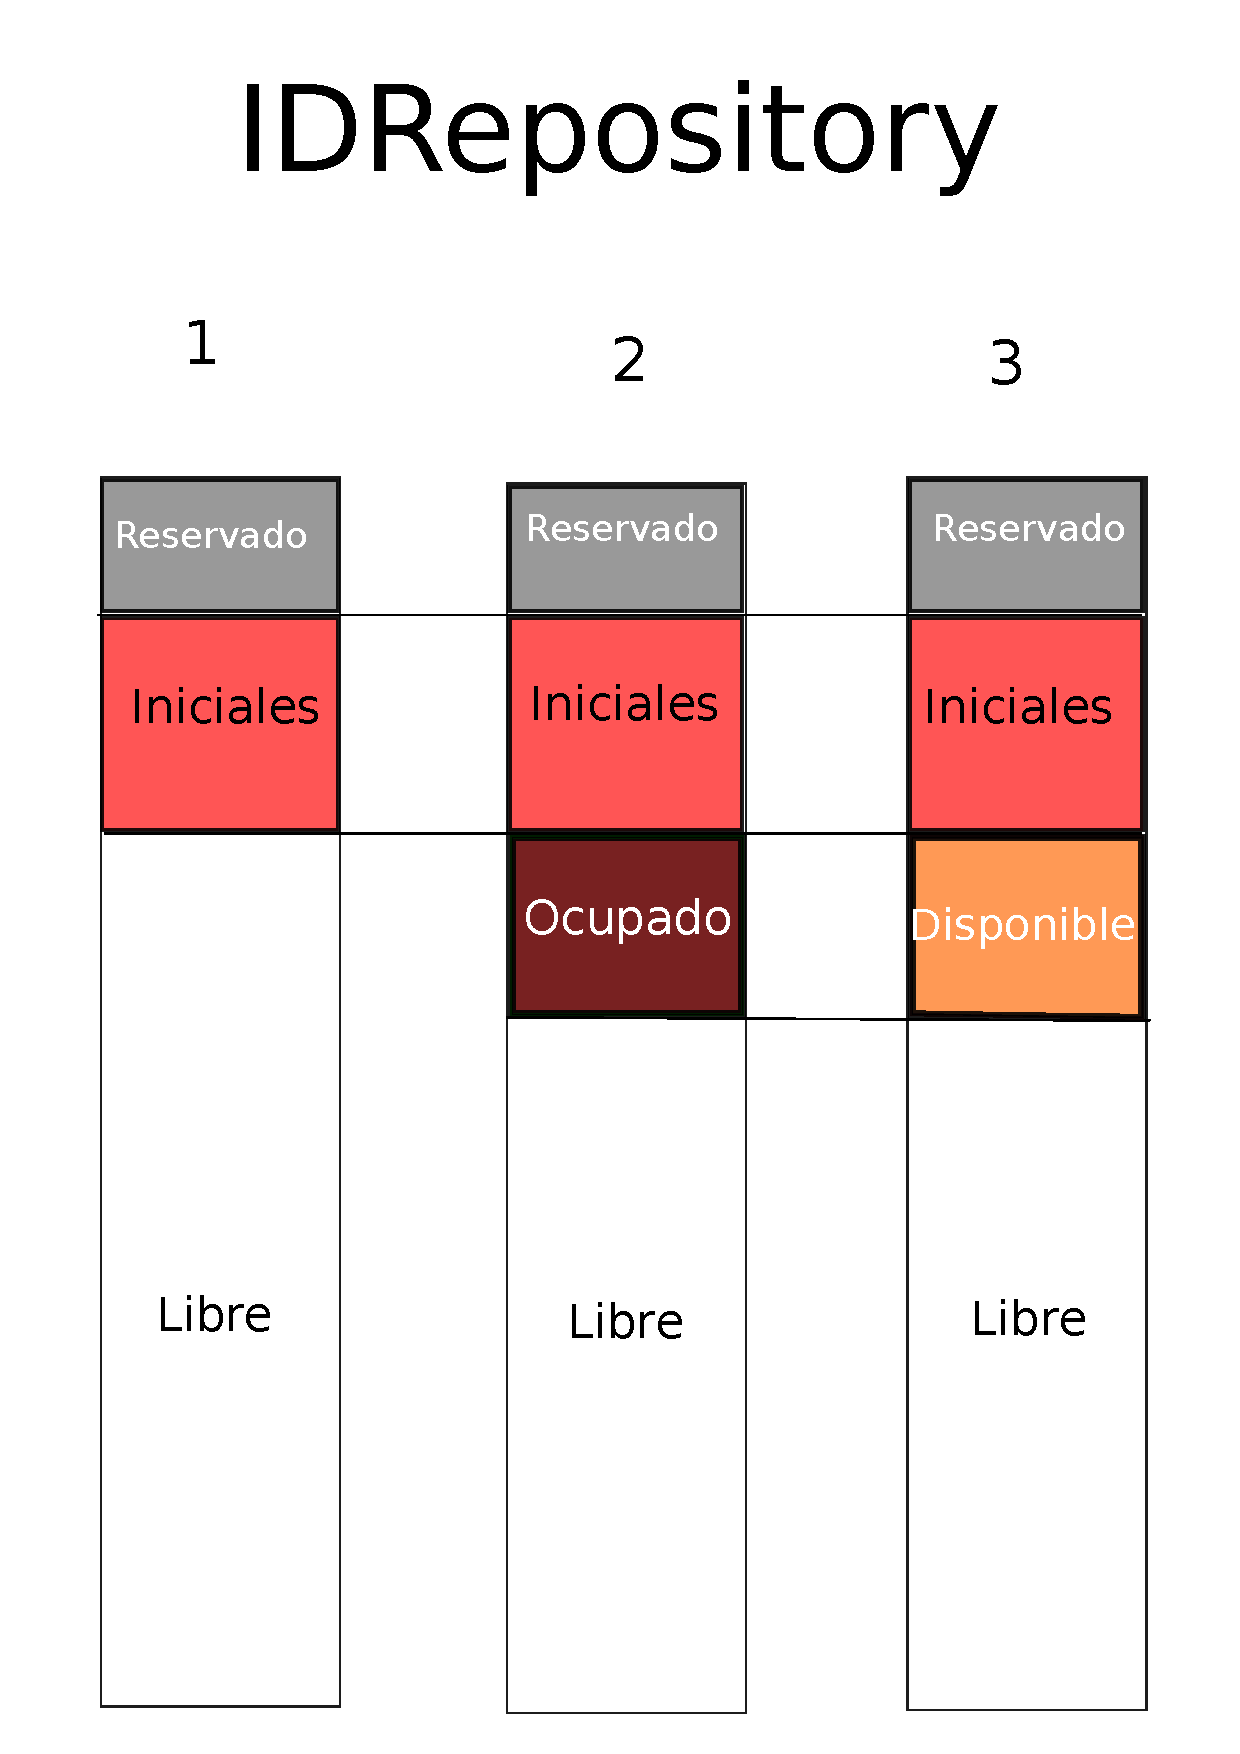
\includegraphics[scale=0.3]{repository.pdf} 
\end{center}
\caption[Forma de trabajo IDRepository]{Se muestra la forma de trabajo de IDRepository y el manejo de su memoria}
\label{repositorylabel}
\end{figure}
En la Figura \ref{repositorylabel} se muestra cómo trabaja IDRepository a través de 3 etapas. En la primera de ellas se muestra el espacio reservado marcado en gris por IDRepository para la gestión de los jugadores y un área ocupada por los objetos iniciales del juego marcada en rojo.

Luego en la etapa 2 se muestra un área ocupada por los objetos en la escena. Posteriormente el área ocupada anterior está disponible para ser reservada por otros objetos. En esta parte el área sigue siendo ocupada en memoria física sin embargo los nuevos objetos no incurrirán en una nueva reserva.

Finalmente el area libre simboliza el área de memoria física no ocupada por IDRepository.
\subsection{Contexto jBomb}
En el juego el traspaso de información es muy variado y para ello lo común es pasar dicha información a través de parámetros a todos los métodos de las clases. Sin embargo existen algunos componentes que son muy utilizados y al pasarlos por parámetros hace el código bastante engorroso dado que debe ser suministrado a la mayoría de los componentes. 

Para solucionar esto existe el contexto de jBomb que se encarga de almacenar toda esta información de manera estática, lo que significa que no es necesario crear instancias de este contexto para hacer uso de esa información, sino basta con llamarlo desde cualquier parte del código sin necesidad de pasarla por parámetro.

La información contenida en el contexto son referencias a algunos componentes antes descritos, estos son:
\begin{description}
\item[AssetManager] Está encargado de cargar los recursos de el módulo de assets, es decir se encarga de cargar las texturas, imágenes y sonidos \cite{BEGINNERS}.
\item[Nodo] Se encarga de almacenar una referencia al nodo raíz (Root Node), es el responsable de mantener visibles todos los objetos Hijos que tenga.
\item[PhysicsSpace] Es una referencia a todo el espacio físico y su función es agrupar todos los objetos que están expuestos a se afectados por las fuerzas de colisiones, gravedad o cualquier interacción física.
\item[BaseGame] Es una referencia al propio módulo que permite un rápido acceso para los demás componentes a la interfaz del juego.
\item[AbstractManager] El contexto mantiene una referencia a \textit{AbstractManager} para que pueda ser consultado sobre la cantidad de mensajes recibidos, asignar o eliminar identificadores a los objetos, etc.
\item[MessagesPerSecond] Almacena la cantidad de mensajes por segundo que serán enviados al servidor por todos los clientes. El número actual es 20 mensajes por segundo \cite{VALVE1}.
\item[ElevatorNode] Es el nodo que agrupa todos los elevadores que existen en el juego para tener un mejor y más fácil acceso a cada uno de ellos.
\newpage
\end{description}
\begin{codigo}
\begin{lstlisting}[language=Java,frame=single,basicstyle=\scriptsize]
	package jbomb.common.game;

	import com.jme3.asset.AssetManager;
	import com.jme3.bullet.PhysicsSpace;
	import com.jme3.scene.Node;
	import jbomb.common.appstates.AbstractManager;
	
	public class JBombContext {
	
	    protected JBombContext() {}
	
	    public static AssetManager ASSET_MANAGER;
	    public static Node ROOT_NODE;
	    public static PhysicsSpace PHYSICS_SPACE;
	    public static BaseGame BASE_GAME;
	    public static AbstractManager<?> MANAGER;
	    public static float MESSAGES_PER_SECOND = 20f;
	    public static Node NODE_ELEVATORS;
	}
\end{lstlisting}
\caption{Contexto de jBomb}
\label{lst8}
\end{codigo}
\section{Módulo Cliente}
Como se dijo antes el módulo común proporciona la mayoría del comportamiento del juego, y el módulo de cliente se encarga específicamente en implementar las diferencias que hacen que el juego funcione justamente como un cliente y no como servidor.
Para esto el módulo de cliente extiende una gran cantidad de clases definidas en el módulo común.

El módulo cliente define 2 estados de aplicación, \textit{RunningClientAppState} y \textit{ClientManager}, y en el caso de ambos éstos ya fueron expuestos. En el caso de los controles hace utilización de todos los definidos en el módulo común y además define uno más que tiene la función de mostrar cierta imágen de aviso cuando alguien ha perdido, este control es \textit{WinnerLoserControl}.

Este control está encargado de mostrar una imágen que indica si un jugador ha ganado o si ha perdido durante 7 segundos, y sólo se limita a hacer dicha función ya que son los Listeners, que serán expuestos en detalle en las proximas secciones, los encargados de llamar a este control.

En el cliente y también en el servidor existen unos componentes llamados Listeners que están atentos a cualquier tipo de mensaje que les llegue desde el servidor. Todos los mensajes están definidos en el módulo común y tienen listeners asociados en el cliente y en el servidor. Además el cliente define unos componentes especiales llamados \textit{Tasks} que son ejecutados por estos Listeners.
\subsection{Listeners}
El módulo del cliente tiene 2 formas distintas de responder a ciertas acciones y para ello define al menos 2 tipos de listeners:
\subsubsection{Listeners de mensajes}
Estos listeners están asociados a todos los mensajes provenientes desde el servidor y desencadenan llamadas a componentes llamados \textit{Tasks}. Todos estos listeners derivan de una clase abstracta llamada \textit{AbstractClientMessageListener} que se encarga de simplificar el proceso de ligamento entre el listener y la \textit{Task}.

A continuación se definen los siguientes listeners de mensajes y su acción task asociada.

\begin{flushleft}
\begin{tabular}{|r|p{8.5cm}|}
\hline
\textbf{CounterListener} & Este listener está escuchando mensajes que tienen relación con el conteo regresivo previo al inicio de la ronda y sirve para alertar al jugador del inicio de éste. \\	
\hline
\textbf{CreatePlayerListener} & Listener encargado de recibir mensajes para luego crear el jugador en el cliente. Este mensaje se realiza luego de que el jugador se ha conectado exitosamente con el servidor. \\	
\hline
\textbf{DamageMessageListener} & Está encargado de controlar el nivel de energía del jugador. Cada vez que el servidor detecta que el jugador ha colisionado con una bomba, éste le envía un mensaje de este tipo. \\	
\hline
\textbf{DeadPlayerListener} & Este listener está encargado de ejecutar ciertas acciones cuando detecta que el jugador ha perdido o cuando otro jugador ha perdido. Entre las acciones llevadas a cabo está el sacar el jugador que ha perdido de el nodo del grafo de la escena, colocar mensajes en pantalla, etc. \\	
\hline
\textbf{ExploitBombListener} & Este listener está encargado de hacer explotar la bomba cuando se ha recibido un mensaje de este tipo. \\	
\hline
\textbf{NewPlayerListener} & Cada vez que hay una nueva conexión entre un cliente y el servidor y éste último está en estado de espera de conexiones, se envía un mensaje que solicita la creación de un nuevo jugador, \textit{NewPlayerListener} se encarga de hacer esto último.\\	
\hline
\textbf{RemovePlayerListener} & Este listener actua cada vez que un jugador ha perdido en la ronda o bien cuando el servidor ha detectado que ya no existe una conexión con el cliente. \\	
\hline
\textbf{StartGameListener} & Una vez que la cuenta regresiva ha terminado el servidor envía un mensaje que indica que la ronda ha comenzado. \textit{StartGameListener} se encarga de iniciar el juego en el cliente. \\	
\hline
\end{tabular}
\end{flushleft}
\begin{flushleft}
\begin{tabular}{|r|p{9.3cm}|}
\hline
\textbf{StartingNewListener} & Una vez que la primera ronda del juego ha terminado el servidor empieza a preparar todo para iniciar la otra ronda, y \textit{StartingNewListener} tiene la tarea de reiniciar las posiciones de algunos objetos de la escenta tales como jugadores y elevadores.\\	
\hline
\textbf{ThrowBombListener} & Cuando un jugador lanza una bomba, primero se le envía un mensaje al servidor sobre dicha acción y éste responde a todos los clientes informando quien está lanzando la bomba y en qué posición.\\	
\hline
\textbf{WinnerListener} & Está encargado de mostrar el mensaje de ganador a los jugadores. \\	
\hline
\end{tabular}
\end{flushleft}
\subsubsection{Listeners de acción}
Los listeners de acción están asociados a acciones del usuario tales como pulsaciones de teclado o pulsaciones del mouse. jBomb define 4 listeners de acción y se describen a continuación:
\begin{description}
\item[BombSecondListener] Anteriormente se describieron varias mecánicas de juegos, entre ellas está la duración de las bombas. \textit{BombSecondListener} se encarga de esta mecánica y cada vez que el jugador pulsa los botones asociados a esta mecánica el listener responde a esto estableciendo la información en el GUI NODE y en la lógica del juego.
\item[CharacterActionListener] Este listener está asociado al movimiento del jugador y tiene participación sólo en el módulo del cliente ya que no interactúa con otro modulo y no manda información al servidor. Este listener responde a las teclas de dirección programadas para el movimiento del jugador, las teclas son W, A, S, D.
\item[ServerConnectionListener] Actualmente se limita sólo a mostrar información valiosa en tiempo de desarrollo (debug) y es mencionado aquí porque forma parte de los listener de acción.
\item[ShootsActionListener] Este listener responde a las pulsaciones del botón isquierdo del mouse y que tienen que ver con el lanzamiento de las bombas. Este listener no es el que se encarga de lanzar directamente las bombas, sino que se limita a ver la disponibilidad de éstas y en caso de haberlas se envía un mensaje al servidor solicitando esta acción.
\end{description}
El cliente además de trabajar con Estados de Aplicación, Controles y Listeners también define su propia clase encargada de realizar todas estas tareas haciendo uso de los componentes antes mencionados, esta clase es \textit{JBombClient} y es derivada de \textit{BaseGame}.

\textit{JBombClient} realiza muchas tareas asociadas con el control de la pantalla e inicialización de variables además de algunas funciones para hacer un reinicio del juego, iniciar GUI NODE con las imágenes por defecto de las bombas, energía de los jugadores, etc. Esta clase se encarga de realizar las tareas necesarias para que el juego funcione en la modalidad del cliente.

El módulo del cliente utiliza todas las variables definidas en el contexto \textit{JBombContext} pero con el mismo propósito con el que se difinió este último, el módulo define otro contexto con variables muy utilizadas y este contexto solo almacena información referente al cliente y es por esta misma razón que puede ser utilizada sólo por este módulo.

El nuevo contexto se llama \textit{ClientContext} y almacena la siguiente información:
\begin{description}
\item[Player] Este es la clase encargada de representar al jugador dentro de la ronda manejada por el servidor y es el jugador visto por los demás clientes.
\item[App] Esta es una referencia directa a \textit{JBombClient} para poder acceder al control directo a todas las funciones que manejan el comportamiento del cliente.
\item[Client] Esta clase es la encargada de realizar toda la comunicación con el servidor, lo que significa que ésta gestiona toda la conexión con el servidor durante la ejecución del juego, y está encargada de enviar todos los mensajes provenientes de cliente, estos mensajes son información sobre el jugador, tales como la posición, las acciones, etc.
\end{description}
\section{Módulo Servidor}
Al igual que el módulo de cliente, éste módulo se encarga de implementar toda la funcionalidad que hace que actúe como servidor. La mayoría del comportamiento está heredado desde el módulo común y aquí sólo se implementan funciones especiales asociadas con todo el control del juego.

Anteriormente en el módulo común se describieron los Estados de Aplicación, cuáles eran sus funciones principales y cuáles de éstos existían en jBomb. Este módulo se encarga de extender la funcionalidad asociada de los dos más importantes estados de aplicación y éstos fueron detallados en el módulo común, \textit{RunningServerAppState} y \textit{ServerManager}. 

Además de esas dos implementaciones el módulo de servidor proporciona dos Estados de Aplicación más, \textit{CounterAppState} y \textit{WaitingAppState}.
\begin{description}
\item[CounterAppState] Se encarga de alertar al cliente sobre el pronto inicio de la primera o siguiente ronda. Para ello el servidor se encarga de mandar mensajes con la cantidad de segundos a esperar, tal cual como una cuenta regresiva.
\item[WaitingAppState] Este estado de aplicación se encarga de realizar la espera de 10 segundos antes de que se inicie la siguiente ronda. Es llamado cuando algún jugador ha ganado la ronda actual.
\end{description}

Además de los Estados de Aplicación definidos antes el módulo de servidor también define algunos controles que tratan con las bombas, jugadores y elevadores. Estos controles son:
\begin{description}
\item[BaseBombControl] Es el control base para las bombas que son gestionadas en el servidor y éste hereda desde \textit{AbstractBombControl}, el cuál está definido en el módulo común. \textit{BaseBombControl} se encarga de implementar la lógica que envía el mensaje de nueva bomba a los clientes conectados y también la que permite saber cúando la explosión de la bomba está colisionando con los jugadores.
\item[ElevatorControl] Este control se encarga de mantener en movimiento todos los elevadores que están en la escena. El comportamiento es subir y bajar los elevadores y esperar de 3 a 5 segundos.
\item[GhostBombControl] Este control se encarga de representar a la explosión de la bomba en la escena de manera que otro componente pueda determinar las colisiones de este control con los jugadores.
\item[ScorePlayerControl] Este control es agregado a todos los jugadores (uno por cada jugador) y se encarga de llevar un seguimiento sobre la energía restante de el jugador asociado. Este control se define solamente en el módulo del servidor dado que es este último el encargado de llevar dicha lógica, la cual es informada posteriormente a todos los clientes y de esa manera todos están al tanto de la energía restante de todos los jugadores participantes de la ronda.
\end{description}
En cuanto a los Listeners el módulo de servidor define al menos cuatro listeners, dos de mensajes y dos de acción. Los listeners de mensajes son los siguientes:
\begin{description}
\item[CreatePlayerListener] Este listener tiene la tarea de recibir los mensajes de conexión inicial de los clientes y llevar un registro con la cantidad actual de clientes conectados, de esta manera el servidor sabrá cuando es la hora de iniciar una nueva ronda.
\item[ThrowBombListener] Está encargado de recibir mensajes de lanzamientos de bombas provenientes de los jugadores. Luego de recibir el mensaje, el listener reune toda la información necesaria para reenviarla a todos los clientes, esta información es sobre la bomba como la posición, la duración y el cliente que la está lanzando.
\end{description}
Los listeners de acción definidos en el servidos son:
\begin{description}
\item[BombCollisionListener] Se encarga de agregar el daño asociado a los jugadores producto de la colisión de la bomba con dicho jugador.
\item[ClientConnectionListener] Se encarga de asignar el color y posición inicial de todos los jugadores en el juego.
\end{description}
El módulo de servidor define el equivalente a \textit{JBombClient} y que también hereda de \textit{BaseGame}, esta clase se llama \textit{JBombServer}. Aquí se concentran gran parte de la lógica pricipal del módulo del servidor en donde hace utilización de todos los componentes antes mencionados. Entre las tareas más importantes están las funciones asociadas para iniciar una nueva ronda, iniciar el tiempo de espera (\textit{WaitingAppState}), gestión de conexiones con clientes, inicio del juego, reinicio del juego, manejo de jugadores, configuración de logs y provisión de implementaciones especiales para controles de elevadores.

Al igual que en el módulo común y en el módulo de cliente este módulo define un contexto llamado \textit{ServerContext} con la finalidad de facilitar el acceso a variables ampliamente utilizadas que sólo tienen sentido dentro del módulo de servidor. Las variables definidas dentro de este contexto se definen en la siguiente tabla:

\begin{flushleft}
\begin{tabular}{|r|p{8.3cm}|}
\hline
\textbf{SERVER} & Almacena una referencia al componente que obtiene la conexión con los clientes y es utilizada por diferentes componentes dentro del módulo con el fin de enviar mensajes a todos los clientes conectados.\\	
\hline
\textbf{NODE\_PLAYERS} & Es un Nodo con todos los jugadores que participan en la ronda y facilita el mantenimiento de éstos para su ubicación en la escena.\\	
\hline
\textbf{PLAYERS\_COUNT} & Almacena la cantidad de jugadores permitidos en la ronda, actualmente está soportado para 2, 3 y 4 jugadores.\\	
\hline
\textbf{APP} & Esta almacena una referencia a la clase \textit{JBombServer} con el fin de gatillar acciones que inician ciertas acciones como por ejemplo el reinicio del juego, inicio de estado de espera, etc.\\	
\hline
\textbf{CONNECTED\_PLAYERS} & Contiene la cantidad de jugadores conectados con el servidor y es utilizada para determinar ciertas acciones en el juego.\\	
\hline
\textbf{ROUND\_FINISHED} & Ésta actúa como una bandera que indica si la ronda actual ha finalizado o no.\\	
\hline
\textbf{CONNECTION\_LIST} & Mantiene una lista de conexiones con los clientes que es usada cuando el servidor termina una ronda y está en condiciones de realizar una inspección del estado actual de todas las conexiones, de esa manera éste puede determinar si es posible empezar con una nueva ronda o es necesario esperar por más conexiones.\\	
\hline
\end{tabular}
\end{flushleft}
\chapter{Sincronización de Jugadores}
Una de las características más importantes del juego es la posibilidad de jugar online con amigos que pueden estar dentro de la misma red o internet. Sin embargo esta característica conlleva un montón de consideraciones que deben ser controladas de manera correcta, algunas de éstas son la latencia \cite{VALVE2} y la sincronización \cite{VALVE1}.

En este capítulo se describe la problemática y la solución utilizada para la sincronización de los clientes, de manera que todos puedan ver lo que está ocurriendo en el juego pero desde distintas posiciones y perspectivas.
\section{Problemática} 
El objetivo principal del servidor es mantener un juego consistente de manera que sea lo mismo para todos. Por esta razón surge la problemática de cómo lograr que todos los clientes conectados puedan percibir el mismo escenario que los demás jugadores. 

Si bien los clientes están todos conectados con el servidor éstos son juegos independientes, por lo que el servidor juega un papel importante dado que debe realizar las funciones necesarios para controlar cierta parte de los clientes.

Por lo anterior el servidor es el encargado de mantener sincronizados a todos los clientes para que éstos puedan ver aquellos objetos que son controlados por éste en su posición correcta en el momento correcto. Para ello el servidor envía mensajes sobre dichos objetos que contienen la información útil para que el cliente pueda tomar dicha información y generar ciertas tareas en base a ella. La información contiene por lo general la posición del objeto y un identificador único dentro del juego conocido por todos los clientes, además de información específica relativa al tipo de mensaje que el servidor esté enviando.

Teniendo los mensajes listos para ser enviados y posteriormente aplicados por los clientes, surge el siguiente problema. La cantidad de información para representar el seguimiento continuo de movimiento de un objeto de la escena no sería tan grande si no fuera por la cantidad de puntos en el espacio que se debe representar. Actualmente el juego trabaja con un máximo de 4 clientes por lo que la cantidad de mensajes se cuadruplica, y debe tenerse en consideración que los clientes están en constante movimiento, e incluso si estos no lo están es necesario que el servidor mantenga informado a todos los clientes sobre dicho estado del objeto.

El tráfico sobre la red es demasiado si a eso se le agrega que por cada jugador puede haber al menos 3 bombas en escena, por lo que la cantidad de objetos aumenta en 12 unidades. 

Cabe mencionar que el flujo de información es en ambos sentidos, todos los clientes están informando al servidor sobre la posición de sus jugadores y el lanzamiento de nuevas bombas, a su vez el servidor está recibiendo dicha información y realiza actualización del trabajo de forma local para que posteriormente esta información pueda ser difundida a través de una función de Broadcast\footnote{Es un término inglés para referirse generalmente a la difusión de información a múltiples destinos a la vez} a todos los clientes.

Para que un juego pueda ser visualizado de manera más menos fluida basta con que tenga sobre 30 [fps] \cite{VALVE1} por lo que el servidor debería enviar al menos 30 mensajes por cada objeto que deba controlar en los clientes en cada segundo (a lo más 4 jugadores y 12 bombas). Además de los objetos mencionados antes, también el juego posee 12 elevadores que son controlados por el servidor, por lo que se suma un total de 28 objetos a ser controlados por el servidor.

Si un juego requiere al menos 30 [fps] para que pueda ser visualizado de manera fluida, esto implica que en cada segundo el servidor debiera informar 30 mensajes sobre la posición de los 28 objetos a todos los clientes, además de controlar y aplicar dicha información de manera local. Esto significa que debiese estar enviando 840 mensajes por segundo a cada cliente, lo que se traduce en 3360 [mensajes / seg] en total. Como si fuese poco, la comunicación es bidireccional por lo que cada cliente está enviando como mínimo a una velocidad de 30 [mensajes / seg] mensajes sobre la posición absoluta del jugador en el escenario.

A pesar de que el problema de mantener coordinados a todos los clientes se ha solucionado, se hace necesario optimizar la forma en como se está sincronizando a los clientes dado que el envío de mensajes no es la única función a lo que se limita el servidor. 
\section{Solución Implementada}
En la sección anterior se propone el envío de mensajes para mantener a los clientes coordinados sobre lo que está pasando en el juego de manera que éstos puedan ver lo mismo desde sus diferentes posiciones y ángulos, es decir existe un componente encargado de mantener actualizados a todos los clientes con la información absoluta sobre la posición de los diferentes objetos en el juego, entre ellos los elevadores, bombas y jugadores.

Al mismo tiempo, se detecta que la información que requiere ser enviada a cada cliente es del orden de 840 [mensajes / seg] y a pesar de que es harta información es probable que la red no se sature con ello pero aún así es necesario optimizar dicho proceso para que el juego pueda escalar sin problemas al aumentar el número de jugadores dentro de la ronda. Los grandes juegos basados en la red utilizan técnicas especiales para tratar con la latencia y el envío de estos mensajes.

Una técnica para reducir el número de mensajes enviados (recibidos) a los (por los) clientes es la Interpolación \cite{VALVE1}.
\subsection{Interpolación} 
La interpolación es un subconjunto de la matemática que se dedica al análisis numérico, el cual permite encontrar nuevos datos a partir de un conjunto de datos discretos. El caso más fácil y conocido es la interpolación lineal.
$$I = At + (1-t)B$$
$A$ y $B$ corresponden a al punto inicial y final respectivamente, con $0 <= t <= 1$ y representa el porcentaje de la distancia entre ambos puntos a la que se desea interpolar, $I$ es el punto interplado.

jBomb hace utilización de la interpolación lineal para reducir el número de mensajes que tienen que ser enviados a los clientes, de esa manera se optimiza la forma en cómo se está controlando a los clientes y permite al servidor dedicar más capacidad de procesamiento a tareas que tienen que ser aplicadas de manera local para llevar un correcto funcionamiento del juego.

El servidor trabaja con objetos que deben ser identificados por todos los clientes, estos objetos deben estar en la posición correcta y en el momento correcto para que los clientes puedan ver el mismo juego a la vez. Todos estos objetos tienen unos identificadores, los cuales son asignados por el servidor, y son comunes en todos los clientes. El identificador es obtenido por el \textit{IDRepository} para que el objeto sea único y así esta información pueda ser contenida dentro del mensaje enviado junto con otra información específica del tipo de mensaje.

Los objetos a ser identificados pueden ser Elevadores, Bombas o Jugadores, sin embargo la interpolación sólo es utilizada por los jugadores y elevadores. Esta diferenciación se da porque las bombas utilizan funciones de movimiento que aprovechan las capacidades del entorno del cliente, el cual integra la simulación de fuerzas de gravedad y permite que la bomba pueda seguir una trayectoria esperada durante su recorrido. Es decir que la información contenida en los mensajes relativos a la bomba no contine posiciones de la bomba, sino dirección y magnitud de la fuerza aplicada a la bomba.

Al ser una fuerza la aplicada sobre las bombas, éstas determinan sus futuras posiciones automáticamente según el espacio físico del cliente. Aún así es posible que la dirección trazada por el espacio físico del cliente para dicha bomba sea diferente al trazado por el servidor localmente, y por esa razón el servidor vuelve a enviar mensajes sobre la aplicación de nuevas fuerzas en determinadas localizaciones a la bomba. Actualmente la frecuencia de envío de mensajes es de 20 por segundo, por lo que en esa fracción de segundo para el usuario es imperceptible las variaciones que podrían generarse entre el servidor y el cliente.

Por otro lado el elevador y los jugadores se mueven en base a posiciones, puntos tridimensionales que deben ser reenviados a todos los clientes y por esta razón se hace necesario enviar una cantidad enorme de mensajes para que el movimiento de estos objetos sea fluido, pero gracias a la interpolación es posible reducir el número de mensajes e interpolar ciertos puntos entre una posición y otra.

La pricipal diferencia en cómo son manejados los elevadores y los jugadores por el servidor, es que éstos últimos se desplazan según los mensajes que estén enviando los clientes dado que son ellos los que dirigen a los jugadores, por lo que el servidor no tiene la potestad de definir las posiciones de los jugadores. 

Por el contrario los elevadores son manejados en todo momento por el servidor y el cliente sólo se limita a actualizar la posición de éstos, mediante la aplicación de la información contenida en los mensajes de los elevadores o bien mediante las técnicas de interpolación.

Para determinar las posiciones de ambos objetos (elevadores y jugadores) se debe aplicar la información contenida en el mensaje correspondiente o bien se debe realizar el procedimiento de la interpolación, en cualquiera de los dos casos los pasos a seguir son los siguientes:
\begin{enumerate}
\item Determinar si es momento de aplicar la información del mensaje o bien utilizar interpolación.
\item Si el tiempo máximo de espera para la interpolación ha terminado, se debe aplicar la información del mensaje e ir al paso 8.
\item Si aún no es tiempo de aplicar la información del mensaje entonces se debe realizar la interpolación.
\item Calcular la proporción que existe entre el tiempo que está acumulado y el tiempo máximo de interpolación.
\item Determinar si es la primera interpolación realizada para dicho mensaje
\item En caso de ser la primera, establecer el punto inicial que corresponde a la posición actual del objeto (el punto final es conocido y está informado en el mensaje) y volver al paso 1.
\item Si no es la primera, se aplica la interpolación a una distancia que corresponde a la proporción calculada en el paso 4 entre el punto inicial establecido en el paso 6 y el punto final que corresponde a la posición informada en el mensaje, luego volver al paso 1.
\item Descartar el mensaje porque su información ya no tiene validez dentro de los proximos segundos.
\end{enumerate}
Las cajas de código \ref{frag1} y \ref{frag2} ilustran la implementación de la interpolación para los mensajes \textit{CharacterMovesMessage} y \textit{ElevatorMovesMessage} respectivamente.
\begin{codigo}
\begin{lstlisting}[language=Java,frame=single,basicstyle=\scriptsize]
	@Override
    public void interpolate(float percent) {
        Player p = (Player) JBombContext.MANAGER.getPhysicObject(getId());
        if (p != null) {
            if (!isFirstInterpolation) {
                oldPosition.set(p.getGeometry().getLocalTranslation());
                isFirstInterpolation = true;
            }
            p.getGeometry().setLocalTranslation(
            FastMath.interpolateLinear(percent, oldPosition, location));
        }
    }
\end{lstlisting}
\caption{Interpolación en \textit{CharacterMovesMessage}}
\label{frag1}
\end{codigo}
\newpage
\begin{codigo}
\begin{lstlisting}[language=Java,frame=single,basicstyle=\scriptsize]
	@Override
    public void interpolate(float percent) {
        Elevator e = (Elevator) 
        	JBombContext.MANAGER.getPhysicObject(getId());
        if (e != null) {
            if (!isFirstInterpolation) {
                oldPosition.set(e.getGeometry().getLocalTranslation());
                isFirstInterpolation = true;
            }
            e.getGeometry().setLocalTranslation(
            FastMath.interpolateLinear(percent, oldPosition, location));
        }
    }
\end{lstlisting}
\caption{Interpolación en \textit{ElevatorMovesMessage}}
\label{frag2}
\end{codigo}
A continuación se explica de forma detallada el proceso de interpolación.
\subsubsection{Paso 1: Mensaje o Interpolación}
El flujo del juego se realiza a través de una cierta cantidad de ciclos por segundo, en donde en cada ciclo el juego muestra una imágen o frame del estado actual del juego. La cantidad de ciclos por segundo no es constante y depende de la capacidad de procesamiento de la CPU o la GPU. Para tener una sensación de juego fluido basta con que se obtengan al menos 30 o más frames por segundo (fps) \cite{VALVE1}. Si decidimos que 30 [fps] son aceptables para que jBomb pueda disfrutarse de una manera aceptable, entonces el servidor debería enviar en cada tick (ciclo) un mensaje de posición a todos los clientes.

Con ayuda de la interpolación podemos reducir este número de mensajes, jBomb se basa en las recomendaciones de Valve \cite{VALVE2} y define un tiempo de interpolación como la fracción 1/20 [segs], es decir a lo más se enviarán 20 mensajes por segundo, siendo estos totalmente independiente de la velocidad del motor gráfico. Entre medio de ese lapso de tiempo, se realizará interpolación cada vez que sea posible.

Por lo tanto, el objetivo de este primer paso es determinar si se debe aplicar el mensaje o bien la interpolación. Para ello basta con observar el tiempo transcurrido desde el último mensaje enviado hasta ahora.
\subsubsection{Paso 2: Aplicación de mensaje}
Este paso corresponde a cuando el tiempo transcurrido es igual o superior al tiempo de interpolación, como se dijo antes este tiempo es de 1/20 [segs]. Si el tiempo transcurrido es mayor a este tiempo, es hora de aplicar la información contenida en el mensaje que es por lo general es el identificador del objeto y la nueva posición del objeto.

Una vez concluido esto, la información del mensaje es irrelevante por lo que el mensaje es descartado, lo que es realizado en el último paso de este algoritmo.
\subsubsection{Paso 3: Interpolación}
Si se ha llegado hasta este punto es porque aún existe tiempo para aplicar la interpolación. Los datos que se deben utilizar son la posición inicial(posición original del objeto antes de realizar cualquier interpolación) y el punto destino (corresponde a la posición informada por el mensaje).

\begin{figure}
\begin{center}
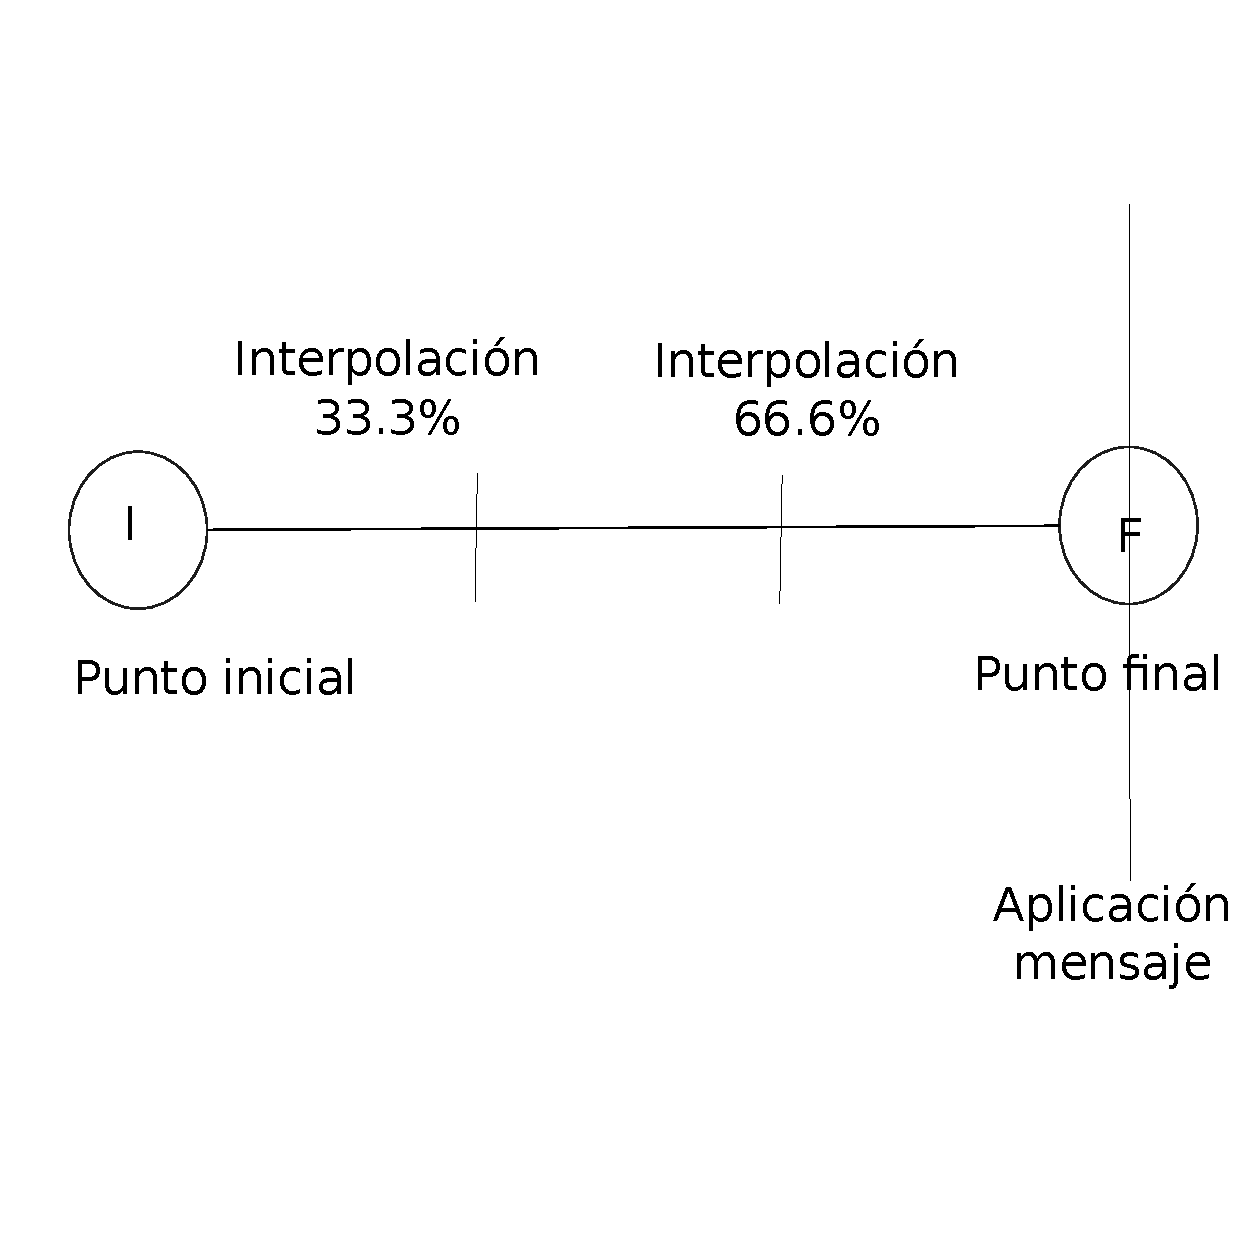
\includegraphics[scale=.7]{interpolacion1.pdf}
\caption[Interpolación de 33.3\% y 66.6\% de avance]{Interpolación de 33.3\% y 66.6\% de avance antes de aplicar la información del mensaje}
\label{interpolacionlabel}
\end{center}
\end{figure}

Teniendo estos dos puntos es posible interpolar los puntos existentes entre ellos sin embargo, antes de determinar cuál será el punto o la distancia a interpolar, se debe calcular dicho valor para que éste pueda ser proporcional a la cantidad de tiempo transcurrido desde la última aplicación del mensaje.

Por ejemplo, si el tiempo transcurrido hasta el momento es de 1/40 [segs] desde la última aplicación del mensaje, este es un medio del tiempo de máximo de interpolación (1/20 [segs]) por lo que lo correcto sería que el objeto esté al menos a la mitad de la distancia entre el punto inicial y el punto final.

En la Figura \ref{interpolacionlabel} se resume de forma gráfica el proceso de interpolación, en donde se determinan 2 puntos antes de aplicar la información final contenida en el mensaje de actualización de posición de algún objeto en la escena.
\subsubsection{Paso 4: Cálculo de proporción}
Esta etapa corresponde al cálculo para determinar cuánto es la candidad que se tendrá que avanzar en la interpolación. El cálculo no es más que una simple división entre la sumatoria de todos los tiempos acumulados de los ciclos transcurridos desde la última aplicación del mensaje y el tiempo máximo de interpolación.
$$\frac{(t_1 + t_2 + t_3 + ... + t_n )}{T}$$
Por ejemplo:

Se tiene un tiempo acumulado de 1/60 [segs] en 3 ciclos, y el tiempo máximo de interpolación es 1/20 [segs], por lo tanto es posible hacer interpolación dado que 1/60 es menor que 1/20, por lo que la proporción es 1/3, lo que equivale a un 33,3\% de avance entre el punto inicial y el punto final.
\subsubsection{Paso 5: Primera interpolación}
Esta etapa ocurre luego de aplicar el mensaje, esto quiere decir que no se ha hecho interpolación y la posición de el objeto en cuestión (bomba o jugador) es determinada por la información contenida en el mensaje, a esto se le denomina aplicación del mensaje.

Luego de aplicar dicho mensaje, el servidor envía un nuevo mensaje conteniendo la información de la siguiente posición del objeto y se inicia nuevamente el ciclo. Dado que en este momento el tiempo acumulado es 0 (ya que es el primer ciclo luego de la aplicación del mensaje) y el punto inicial no ha sido establecido.
\subsubsection{Paso 6: Punto inicial}
En la etapa anterior se determina si es o no la primera interpolación realizada luego de haber aplicado algún mensaje, de ser así el punto inicial no ha sido establecido. Se debe actualizar este punto para que luego en el siguiente ciclo se pueda interpolar según el tiempo transcurrido entre este ciclo y el siguiente. El punto inicial entonces se convierte en la posición actual del objeto y el punto final es el que viene informado en el contenido del mensaje.
\subsubsection{Paso 7: Aplicación de interpolación}
En este punto es donde realmente se determina la posición del objeto en cuestión. La interpolación utilizada es la interpolación lineal, que permite a través de la ecuación de una recta determinar un punto entre el punto inicial y el punto final. 
$$Y = aX + b$$
La interpolación es utilizada en base a una función proporcionada por el motor de juegos a la cual se le envían 3 parámetros, una es la distancia a la que se desea interpolar, el segundo parámetro es el punto inicial y finalmente el tercer parámetro es el punto final. Como resultado esta función retorna la posicíon en el espacio que será utilizado para determinar la posición actual del objeto.
\subsubsection{Paso 8: Descarte de mensaje}
Una vez que se ha concluido con el tiempo de interpolación, ya es hora de aplicar el mensaje. Una vez realizado este paso, el mensaje ya no tiene validez dado que ya fue utilizado para su propósito y por tanto éste debe ser descartado.
\chapter{Pruebas y Resultados}
jBomb fue desarrollado para trabajar sobre la red y por ende el software está propenso a múltiples errores que están ligados a este tema. Sin embargo con el objetivo de detectar este tipo de problemas sobre la red, y también algunos en general, se han realizado múltiples pruebas.
jBomb ofrece una jugabilidad de 2 personas mínimo y un máximo de 4. Las pruebas han sido realizadas sobre todas las modalidades.

Éstas fueron para verificar el correcto funcionamiento del juego y garantizar que cumple con su contrato y sus mecánicas de juego. Para ello jBomb se puso en funcionamiento en diversas modalidades, esto quiere decir que se ejecutó para trabajar con 2 jugadores, 3 jugadores y 4 jugadores a la vez. El servidor funcionó en sus dos modalidades, en modo gráfico y en modo silencioso. Las pruebas fueron realizadas tanto de forma local, en red local y en internet.

El comportamiento del juego en general fue el esperado, en la mayoría de los casos presentó un funcionamiento normal dentro de lo esperado, cumple con todas sus funciones y logra sus objetivos propuestos en este proyecto, pero en algunos casos se presentan comportamientos anómalos.

A priori, los comportamientos anómalos han sido atribuidos a problemas de red que no han sido completamente bien manejados por el juego y posiblemente requerirán de una intervención más adelante como trabajo futuro. Este tipo de comportamiento extraño se observó en un 10\% de los casos.

Los problemas de este tipo se presentan sólo en algunas oportunidades y los casos varían mucho entre ellos, por ejemplo uno de los casos más vistos fue la gestión de las bombas en el escenario. Cuando un jugador lanza la bomba, el módulo del cliente verifica la factibilidad de enviar la bomba, si es posible hacerlo se envía un mensaje al servidor sobre dicha solicitud. El servidor hace un broadcast de dicho mensaje a todos los clientes y posteriormente realiza esa petición en su juego local (que es el juego llevado a cabo por el servidor y que es lo que todos los jugadores deberían ver desde distintas perspectivas, es como una vista objetiva del juego).

Cuando el mensaje de lanzamiento de bomba ha sido recibido por el cliente (todos los clientes), se procede a realizar dicha función, que es lanzar dicha bomba en alguna posición y en alguna dirección. Sin embargo, por alguna razón hay algunas ocasiones en que el cliente no recibe el mensaje y producto de ello éste no ve nunca una bomba, y esto hace que no todos los cliente estén sincronizados porque no están viendo lo mismo.

En consecuencia de lo anterior, se produce un nuevo error cuando llega el mensaje de explosión de bombas. Cuando el servidor determina que es momento de hacer explotar una bomba en su juego local, debe enviar dicho mensaje a todos los clientes para que estén sincronizados, sin embargo en el cliente que no había recibido el mensaje anterior (el mensaje de lanzamiento de bomba) pueden suceder dos cosas, si no se recibe este nuevo mensaje no sucederá nada y el cliente nunca se habrá dado por aludido que una bomba que si debió estar en el juego no estuvo, o bien si recibe el mensaje se gatillará una excepción de error dado que está recibiendo la orden de explotar una bomba con un id que él desconoce dado que nunca se dió por enterado de que debía haber una bomba con ese id.

Otro caso observado sucedía cuando los jugadores lanzaban bombas pero ésto no se veía reflejado en el juego, se presionaba el botón de lanzar bomba pero no sucedía nada. Luego de un rato, el escenario se llenaba de todas las bombas lanzadas anteriormente y llegaba en escenario de explosiones. Esto también se piensa que es un problema de red.

Lo anterior puede deberse a que el servidor no está enviando los mensajes, esto se concluye porque en ninguno de los clientes los mensajes de bombas fueron recibidos y eso puede deberse a que el servidor está ocupado trabajando con la recepción de los mensajes de bombas, una vez finalizado con ello, éste se dispone a hacer el broadcast de todos los mensajes.

Existe también la posibilidad de que no necesariamente sea el juego el causante estas situaciones extrañas, también podría ser el router o switch utilizado. Muchas veces el router/switch no tiene la capacidad de recibir/enviar tantos mensajes a la vez y posiblemente ese sea el cuello de botella que esté causando estos problemas, e incluso la falla de hardware, interferencia electromagnética, etc pueden ser también causantes de esta problemática.

Otra posible causa sea la utilización del protocolo de tranporte utilizado hasta el momento. Por defecto el protocolo utilizado por jBomb en sus mensajes es TCP\footnote{Del inglés, Transmission Control Protocol (\textit{Protocolo de control de transmisión})}, el cual es un protocolo que garantiza el orden y recibimiento de todos los mensajes enviados y puede deberse justamente a esto que hace que se produzca un retardo en la recepción de los mensajes, lo que causa que el juego no se comporte como debiese.

Una mejor alternativa y posible solución sería el uso del protocolo UDP\footnote{Del inglés, User Datagram Protocol (\textit{Protocolo de datagramas de usuario})}, el cual no garantiza el orden ni el recibimiento de los mensajes. Posiblemente la mejor opción sea una utilización mixta, dado que la importancia del mensaje difiere entre unos y otros.

Estos fueron los problemas descubiertos en algunas oportunidades cuando se realizaron las pruebas. Cabe mencionar que estas anomalías se presentaron sólo en un 10\% de los casos. En resumen, los problemas aquí presentados son a causa del trabajo en red que cualquier software que trabaje sobre ella está obligado a lidiar este tipo de situaciones.
\chapter{Conclusión y Trabajo Futuro}
Actualmente el juego se encuentra en una versión estable y con algunos detalles menores que pueden ser solucionados, los cuales están siempre dentro del ciclo de vida de cualquier software.

Como se menciona en capítulos anteriores el juego posee múltiples caracterísicas que fueron definidas como parte del objetivo general de este proyecto, sin embargo el juego posee algunas falencias que podrían ser tratadas en versiones posteriores, un ejemplo claro es el soporte de múltiples escenas, soporte para jugadores manejados por computadora a través de la Inteligencia Artificial, soporte para mayor número de participantes, características que afecten el comportamiento del juego tales como posiones de vida, trampas, efectos que alteren la escena, etc. 

Las posibilidades de extender el juego son infinitas y están limitadas únicamente por la imaginación de quien desee modificar este proyecto. El proyecto es software libre bajo licencia GNU GPLv3 y por tanto se puede modificar, vender, extender, restringir o cualquier cosa que desee la persona interesada.

Cabe mencionar que algunos ejemplos de futuras características que se mencionaron pueden involucrar más trabajo del esperado y esto responde a que el juego no fue desarrollado de manera modular, sinó que trabaja de manera muy dependiente entre la escena, jugabilidad y lógica del juego.

El caso más representativo de ésto sería el soporte de múltiples escenas, dado que el juego está basado únicamente en una escena y no ofrece posibilidad de cambio de ésta, en consecuencia el desarrollador que desee abordar esta problemática probablemente se verá enfrentado tambíen a el desarrollo de un módulo que se dedique exclusivamente al soporte de escenas, y no sólo al desarrollo de una escena en particular.

A pesar de que cualquier persona está en el derecho de participar en la modificación del proyecto, es necesario contar con un mínimo de experiencia en Java ya que es la tecnología utilizada por jBomb, y adicionalmente se requiere un conocimiento medio sobre motores gráficos para juegos y en particular sobre JMonkeyEngine.

También como trabajo futuro queda la solución a las problemáticas de red presentadas en el capítulo anterior, si bien son un 10\% de los casos presentados en las pruebas, un juego debe minimizar al máximo cualquier tipo de error y sobre todo los que están relacionados con problemas de red \cite{VALVE2}, de esa manera los jugadores podrán sentir que el juego es estable dentro de todas las posibilidades que se pueden dar al tratar con software que funcionan en la red e internet.

También se propone cambiar los protocolos utilizados para el transporte de los mensajes, dado que algunos tienen distintos tipos de importancia sería bueno acomodar el protocolo según el mensaje que se esté enviando \cite{VALVE1}. Esto mejoraría sin lugar a dudas enormemente los detalles tratados en el capítulo anterior.

jBomb ha sido un gran esfuerzo y ha demostrado que el desarrollo de un videojuego es un proceso a largo plazo, un proyecto de gran envergadura y que demanda muchas capacidades y cualidades que pueden ser satisfechas sólo entre un gran equipo. A pesar de que el juego fue desarrollado entre 2 participantes principales en el área de programación y diseño, la experiencia ha demostrado que la necesidad de incorporar profesionales en otras areas ayuda enormemente al desarrollo de éste.

Esto se debe a que el fin de jBomb es ser un juego entretenido que pueda ser disfrutado por un grupo de amigos, y para ello se necesita muchas capacidades y habilidades de los desarrolladores para que puedan cumplir con las altas expectativas de los jugadores actuales, pero por sobre todo el gran valor agregado puede ser sólo proporcionado por el conjunto de características que éste pueda proveer a través de la música, los gráficos y la historia detrás del juego. Para llenar el juego de tales características se hace indispensable contar con un equipo conformado por gente especializada en diversas áreas, todos pueden aportar valor agregado al juego a través de ideas que pueden ser implementadas por las diferentes capacidades de los integrantes.

Sin embargo a pesar de que jBomb fue desarrollado por 2 integrantes más 2 colaboradores en la parte de audio y gráficos, ofrece cualidades que son muy significativas y que están presentes en cualquier juego comercial reconocido, además jBomb fue desarrollado con propócitos universitarios y ofrece lo mismo que un juego gratuito, libre o comercial.

Por último jBomb cumple con todos los objetivos propuestos por este proyecto y es considerado un éxito por ello. Su desarrollo no fue fácil, exigió el aprendizaje de nuevas tecnologías, el fortalecimiento de las ya obtenidas y una gran cantidad de trabajo involucrado para que éste pudiese ser considerado como un juego. No hay duda que si se propone, el mismo equipo podria desarrollar un mejor juego dado que se cuenta con la experiencia y el conocimiento básico para un nuevo proyecto de éste equipo, además esta vez se aprendería de los errores cometidos con jBomb y se implementaría un diseño basado en modularidad y abarcando objetivos más orientados a la extensibilidad del juego sin dejar de lado las características que cualquier juego de calidad demandaría.
\bibliographystyle{plain}
\bibliography{bib}
\end{document}